%%%%%%%%%%%%%%%%%%%%%%%%%%%%%%%%%%%%%%%%%%%%%%%%%%%%%%%%%%%%%%%%%%%%%%%
%
%  A small sample UNSW Honours Thesis file.
%  Any questions to Ian Doust i.doust@unsw.edu.au
%
% Edited CSG 11.9.2015, use some of Gery's ideas for front matter; add a conclusion chapter.
%%%%%%%%%%%%%%%%%%%%%%%%%%%%%%%%%%%%%%%%%%%%%%%%%%%%%%%%%%%%%%%%%%%%%%%
%
%  The first part pulls in a UNSW Thesis class file.  This one is
%  slightly nonstandard and has been set up to do a couple of
%  things automatically
%
 
\documentclass[honours,12pt]{unswthesis}
\linespread{1.3}
\usepackage{kotex}
\usepackage{amsfonts}
\usepackage{subcaption}
\captionsetup{compatibility=false}
\usepackage{amssymb}
\usepackage{hyperref}
%\usepackage[nameinlink,capitalise]{cleveref}
\usepackage{amsthm}
\usepackage{latexsym,amsmath}
\usepackage{graphicx}
\usepackage{pgfplots}
\usepackage{afterpage}
\usepackage[ ]{algorithm2e}
\usepackage{bm}
\usepackage{tikz}
\usetikzlibrary{bayesnet}
\usepackage{boondox-cal}
\usepackage{cite}
\usepackage[square]{natbib}
\allowdisplaybreaks[1]
%%%%%%%%%%%%%%%%%%%%%%%%%%%%%%%%%%%%%%%%%%%%%%%%%%%%%%%%%%%%%%%%%
%
%  The following are some simple LaTeX macros to give some
%  commonly used letters in funny fonts. You may need more or less of
%  these
%
\newcommand{\R}{\mathbb{R}}
\newcommand{\Q}{\mathbb{Q}}
\newcommand{\C}{\mathbb{C}}
\newcommand{\N}{\mathbb{N}}
\newcommand{\F}{\mathbb{F}}
\newcommand{\PP}{\mathbb{P}}
\newcommand{\T}{\mathbb{T}}
\newcommand{\Z}{\mathbb{Z}}
\newcommand{\B}{\mathfrak{B}}
\newcommand{\BB}{\mathcal{B}}
\newcommand{\M}{\mathfrak{M}}
\newcommand{\X}{\mathfrak{X}}
\newcommand{\Y}{\mathfrak{Y}}
\newcommand{\CC}{\mathcal{C}}
\newcommand{\E}{\mathbb{E}}
\newcommand{\cP}{\mathcal{P}}
\newcommand{\cS}{\mathcal{S}}
\newcommand{\A}{\mathcal{A}}
\newcommand{\ZZ}{\mathcal{Z}}
%%%%%%%%%%%%%%%%%%%%%%%%%%%%%%%%%%%%%%%%%%%%%%%%%%%%%%%%%%%%%%%%%%%%%
%
% The following are much more esoteric commands that I have left in
% so that this file still processes. Use or delete as you see fit
%
\newcommand{\var}{\mathop{\rm var}}
\newcommand{\Var}{\mathrm{Var}}
\newcommand{\ltp}{\mathrel{{\prec}_p}}
\newcommand{\lep}{\mathrel{{\preceq}_p}}
\def\brack#1{\left \{ #1 \right \}}
\def\bul{$\bullet$\ }
\def\cl{{\rm cl}}
\let\del=\partial
\def\enditem{\par\smallskip\noindent}
\def\implies{\Rightarrow}
\def\inpr#1,#2{\t \hbox{\langle #1 , #2 \rangle} \t}
\def\ip<#1,#2>{\langle #1,#2 \rangle}
\def\lp{\ell^p}
\def\maxb#1{\max \brack{#1}}
\def\minb#1{\min \brack{#1}}
\def\mod#1{\left \vert #1 \right \vert}
\def\norm#1{\left \Vert #1 \right \Vert}
\def\paren(#1){\left( #1 \right)}
\def\qed{\hfill \hbox{$\Box$} \smallskip}
\def\sbrack#1{\Bigl \{ #1 \Bigr \} }
\def\ssbrack#1{ \{ #1 \} }
\def\smod#1{\Bigl \vert #1 \Bigr \vert}
\def\smmod#1{\bigl \vert #1 \bigr \vert}
\def\ssmod#1{\vert #1 \vert}
\def\sspmod#1{\vert\, #1 \, \vert}
\def\snorm#1{\Bigl \Vert #1 \Bigr \Vert}
\def\ssnorm#1{\Vert #1 \Vert}
\def\sparen(#1){\Bigl ( #1 \Bigr )}
\DeclareMathOperator*{\argmin}{arg\,min}
\DeclareMathOperator*{\argmax}{arg\,max}
\newcommand\blankpage{%
    \null
    \thispagestyle{empty}%
    \addtocounter{page}{-1}%
    \newpage}

%%%%%%%%%%%%%%%%%%%%%%%%%%%%%%%%%%%%%%%%%%%%%%%%%%%%%%%%%%%%%%
%
% These environments allow you to get nice numbered headings
%  for your Theorems, Definitions etc.  
%
%  Environments
%
%%%%%%%%%%%%%%%%%%%%%%%%%%%%%%%

\newtheorem{theorem}{Theorem}[section]
\newtheorem{lemma}[theorem]{Lemma}
\newtheorem{proposition}[theorem]{Proposition}
\newtheorem{corollary}[theorem]{Corollary}
\newtheorem{conjecture}[theorem]{Conjecture}

\newtheorem{remark}[theorem]{Remark}
\newtheorem{question}[theorem]{Question}
\newtheorem{notation}[theorem]{Notation}
\numberwithin{equation}{section}
\theoremstyle{definition}
\newtheorem{definition}[theorem]{Definition}
\newtheorem{example}[theorem]{Example}
%%%%%%%%%%%%%%%%%%%%%%%%%%%%%%%%%%%%%%%%%%%%%%%%%%%%%%%%%%%%%%%%%%
%
%  If you've got some funny special words that LaTeX might not
% hyphenate properly, you can give it a helping hand:
%
\hyphenation{Mar-cin-kie-wicz Rade-macher}

%%%%%%%%%%%%%%%%%%%%%%%%%%%%%%%%%%%%%%%%%%%%%%%%%%%%%%%%%%%%%%%%%%
% 
% OK...Now we get to some actual input.  The first part sets up
% the title etc that will appear on the front page
%
%%%%%%%%%%%%%%%%%%%%%%%%%%%%%%%%%%%%%%%%%%%%%%%%%%%%%%%%%%%%%%%%%

\title{Density Ratio Estimators for Variational Methods in Bayesian Neural Networks}

\authornameonly{Alexander Lam}

\author{\Authornameonly\\{\bigskip}Supervisor: Professor Scott Sisson}

\copyrightfalse
\figurespagefalse
\tablespagefalse

%%%%%%%%%%%%%%%%%%%%%%%%%%%%%%%%%%%%%%%%%%%%%%%%%%%%%%%%%%%%%%%%%
%
%  And now the document begins
%  The \beforepreface and \afterpreface commands puts the
%  contents page etc in
%
%%%%%%%%%%%%%%%%%%%%%%%%%%%%%%%%%%%%%%%%%%%%%%%%%%%%%%%%%%%%%%%%%%

\begin{document}

\beforepreface

\afterpage{\blankpage}

% plagiarism

\prefacesection{Plagiarism statement}

\vskip 10pc \noindent I declare that this thesis is my
own work, except where acknowledged, and has not been submitted for
academic credit elsewhere. 

\vskip 2pc  \noindent I acknowledge that the assessor of this
thesis may, for the purpose of assessing it:
\begin{itemize}
\item Reproduce it and provide a copy to another member of the University; and/or,
\item Communicate a copy of it to a plagiarism checking service (which may then retain a copy of it on its database for the purpose of future plagiarism checking).
\end{itemize}

\vskip 2pc \noindent I certify that I have read and understood the University Rules in
respect of Student Academic Misconduct, and am aware of any potential plagiarism penalties which may 
apply.\vspace{24pt}

\vskip 2pc \noindent By signing 
this declaration I am
agreeing to the statements and conditions above.
\vskip 2pc \noindent
Signed: \rule{7cm}{0.25pt} \hfill Date: \rule{4cm}{0.25pt} \newline
\vskip 1pc

\afterpage{\blankpage}

% Acknowledgements are optional


\prefacesection{Acknowledgements}

{\bigskip}Scott Sisson, Edwin Bonilla, Louis Tiao

{\bigskip\noindent}Trevor Trotman

{\bigskip\noindent}Honours Room Inhabitants, esp. Bouldering crew

{\bigskip\noindent}Discord Group+Kong+Brian

{\bigskip\noindent}Sunchit

{\bigskip\noindent}누나

{\bigskip\noindent}Family

{\bigskip\bigskip\bigskip\noindent} Lammy, 11 September 2018.

\afterpage{\blankpage}

% Abstract

\prefacesection{Abstract}
Never use ReLU output to estimate density ratios.\\
Class probability estimator = good, direct density ratio and direct log density ratio estimators = bad.\\ 
Also KL Divergence $>$ "CPE" Divergence for formulating estimator loss function but we already know that (although everyone seems to continue to use CPE divergence).
\afterpage{\blankpage}


\afterpreface

%%%%%%%%%%%%%%%%%%%%%%%%%%%%%%%%%%%%%%%%%%%%%%%%%%%%%%%%%%%%%%%%%%
%
% Now we can start on the first chapter
% Within chapters we have sections, subsections and so forth
%
%%%%%%%%%%%%%%%%%%%%%%%%%%%%%%%%%%%%%%%%%%%%%%%%%%%%%%%%%%%%%%%%%%

\afterpage{\blankpage}

\chapter{Introduction}\label{s-intro}


\section{Problem Context}
In machine learning, particularly for high dimensional applications such as image analysis, it is often desirable to build generative models, so that we can represent the data in lower dimensions via representation learning, and generate new data similar to the examples in our dataset. Assume our dataset $X=\{x^{(i)}\}^N_{i=1}\sim q^*(x)$ is $N$ i.i.d. samples of random variables $x$. Also assume $x$ can be generated by a stochastic process from a latent continuous random variable $z$. These models involve a posterior distribution $p(z|x)$ that maps the dataset $x$ to lower dimensional latent prior $z$ (e.g. $z\sim N(\mu,\Sigma)$) then simulating from the prior $p(z)$ to generate new data through a decoder parametrized by $\theta$ $p_\theta(x|z)$. In this particular field, there are three main problems to solve:
\begin{enumerate}
\item Estimation of $\theta$, so that we can actually generate new data $x$
\item Evaluation of the posterior density $p(z|x) = \frac{p(z)p_\theta(x|z)}{p(x)} = \frac{p(x|z)p(z)}{\int_z p(x,z)dz}$, so we can encode our data $x$ in an efficient representation $z$
\item Marginal inference of $x$ ie. evaluating $p(x)$, so it can be used as a prior for other tasks
\end{enumerate}
This problem is analogous to a typical Bayesian inference problem, in which $z$ is the parameter we want to perform inference on, and $x$ is the dataset. We have a distribution which represents our prior beliefs $p(z)$ and a likelihood distribution $p(x|z)$, and we want to determine the posterior distribution $p(z|x)$.



%%%%%%%%%%%%%%%%%%%%%%%%%%%%%%%%%%%%%

\chapter{Background on Neural Networks}
In this chapter we give a general overview of a common model used in deep learning: neural networks. We first explain the motivation and intuition behind the model, then we describe the structure of an individual node. We then expand to the overall neural network structure, and after describing the network initialisation method, we conclude the chapter by demonstrating gradient descent training of neural networks and how back-propagation is used to find the required partial derivatives.
\section{Motivation}
Originally, neural networks were an attempt to create an algorithm that mimics the human brain's method of solving problems. The first machines using a neural network structure were created in the 1950s, and they were used widely from the 1980s onwards, as computers became sufficiently powerful for network training \citep{DeepLearning}.

One key feature of the brain structure is the capability of the neurons to adapt to suit different purposes\cite{neuroplast}. Neuroscientists have conducted experiments on animals where they rewired the optic nerve from the eye to the auditory cortex. They found that the auditory cortex eventually adapted to process the visual signals, and the animals were able to perform tasks requiring sight. This experiment can be repeated for almost any input sensor and the neurons will adjust accordingly to process the signals in a useful manner. They deduced that each neuron has a similar structure regardless of its location in the brain, in which electrical signal inputs are transformed in some way and outputted to other neurons. Overall, the network of neurons was able to process an arbitrary input signal to suit a given purpose\cite{neuroplast}. These are the core principles behind neural network models.
\newpage
Let $f^*$ be some function in the space of $\R$. The primary goal of a neural network is to approximate $f^*$ using a mapping with parameters $\bm{\Theta}$ from input $\bm{x}$ to output $\bm{y}$: $\bm{y}=\bm{f}_{\bm{\Theta}}(\bm{x})$ \citep{DeepLearning}. In fact, the universal approximation theorem states that neural networks can approximate any function in a finite-dimensional space with any desired non-zero amount of error, provided they are complex enough \citep{universal, cybenko}. For example, a typical regression problem of estimating housing prices would have the network inputting the values of certain predictors such as size (continuous) and type of building (categorical), and outputting the expected price. Another example is the classification problem of recognising handwritten digits (0-9) in a black and white image \citep{mnist}. There would be many inputs corresponding to the value of each pixel, and the network would have 10 outputs corresponding to the probability of each digit, and the digit with the highest probability is then selected.
\section{Individual Node Structure}
Before discussing the overall structure of the neural network, we describe the structure of an individual node. A typical node takes in inputs from either the external input, or the outputs from other nodes, in addition to a bias node, which has the same purpose as the intercept term in a regression problem. The nodal inputs $\bm{x}$ are multiplied by weights $\bm{\theta}$ and then passed through an activation function $g(\bm{x})$. The individual node function is therefore \[h_{\bm{\theta}}(\bm{x})=g\left(\sum\limits^n_{i=0}\theta_ix_i\right)\] where n is the number of inputs excluding the bias node, which always has constant value $x_0=1$ \citep{neuralstat}. An example of this is given in Figure 2.1 on the next page. 

The objective of the activation function is to map the network output, possibly non-linearly, to a given range, such as $(0,1)$ or $\R$. This mapping restricts the output range and determines how much input signal is needed before the output becomes asymptotically large \citep{haykin}. A list of common activation functions is given in Section 2.3.
\begin{figure}[h!]
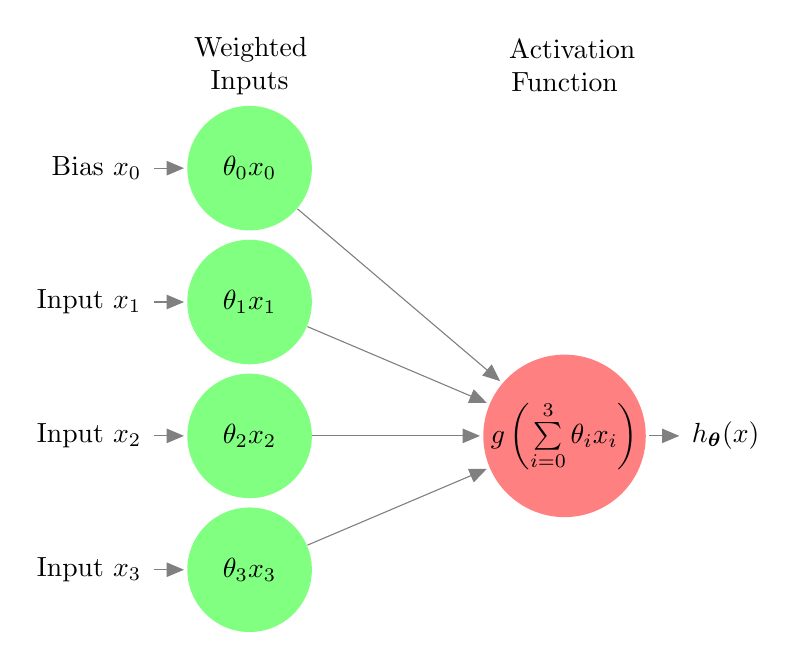
\begin{tikzpicture}[shorten >=1pt,->,draw=black!50, node distance=2.5cm]
    \tikzstyle{every pin edge}=[<-,shorten <=1pt]
    \tikzstyle{neuron}=[circle,fill=black!25,minimum size=45pt,inner sep=0pt]
    \tikzstyle{input neuron}=[neuron, fill=green!50];
    \tikzstyle{output neuron}=[neuron, fill=red!50];
    \tikzstyle{hidden neuron}=[neuron, fill=blue!50];
    \tikzstyle{annot} = [text width=4em, text centered]

    % Draw the input layer nodes
 %   \foreach \name / \y in {0,...,3}
    % This is the same as writing \foreach \name / \y in {1/1,2/2,3/3,4/4}
        \node[input neuron, pin=left:Bias $x_0$] (I-0) at (0,-0) {$\theta_0 x_0$};
	\foreach \name / \y in {1,...,3}
    % This is the same as writing \foreach \name / \y in {1/1,2/2,3/3,4/4}
        \node[input neuron, pin=left:Input $x_{\y}$] (I-\name) at (0,-1.7*\y) {$\theta_{\y}x_\y$};
    % Draw the hidden layer nodes
    %\foreach \name / \y in {1,...,5}
     %   \path[yshift=0.5cm]
      %      node[hidden neuron] (H-\name) at (\layersep,-\y cm) {};

    % Draw the output layer node
    \node[output neuron,pin={[pin edge={->}]right:$h_{\bm{\theta}}(x)$}, right of=I-2, node distance=4cm] (O) {$g\left(\sum\limits^3_{i=0}\theta_ix_i\right)$};

    % Connect every node in the input layer with every node in the
    % hidden layer.
   % \foreach \source in {1,...,4}
    %    \foreach \dest in {1,...,5}
     %       \path (I-\source) edge (H-\dest);

    % Connect every node in the hidden layer with the output layer
    \foreach \source in {0,...,3}
        \path (I-\source) edge (O);

    % Annotate the layers
%    \node[annot,above of=H-1, node distance=1cm] (hl) {Hidden layer};
    \node[annot,above of=I-0, node distance=1.3cm](il) {Weighted Inputs};
    \node[annot,right of=il, node distance=4cm] {Activation Function};
\end{tikzpicture}
\caption{\small Example structure of an individual node function with 3 inputs, labelled as $\bm{x}=[x_0\quad x_1\quad x_2\quad x_3]^\top$, with $x_0$ corresponding to the bias node. The weights are denoted as $\bm{\theta}=[\theta_0\quad \theta_1\quad \theta_2\quad \theta_3]$.}

\end{figure}
\newpage
\section{Activation Functions}
Some common activation functions are \citep{DeepLearning}:
\begin{itemize}
\item The rectified linear unit or ReLU activation function output is bound in $[0,\infty)$. It has the formula $g(x)=\max\{0,x\}$ corresponding to node function $h_{\bm{\theta}}(\bm{x})=\max\{0,\bm{\theta}^\top\bm{x}\}$.
\item The sigmoid or logistic activation function outputs are restricted to $(0,1)$, with the formula $g(x)=(1+\exp(-x))^{-1}$ corresponding to node function  $h_{\bm{\theta}}(\bm{x})=(1+\exp(-\bm{\theta}^\top\bm{x}))^{-1}$.
\item The hyperbolic tangent function output ranges between $(-1,1)$, denoted as $g(x)=\tanh(x)$ corresponding to $h_{\bm{\theta}}(\bm{x})=\tanh(\bm{\theta}^\top\bm{x})$.
\item The linear activation function is used to describe nodes with no activation function, as it's formula is $g(x)=x$, corresponding to $h_{\bm{\theta}}(\bm{x})=\bm{\theta}^\top\bm{x}$.
\end{itemize}
Their plots are shown in Figure 2.2 on the next page.\\
\begin{figure}[h]
\resizebox{\textwidth}{!}{
\begin{tikzpicture}
\begin{axis}[name=ReLU, xlabel=$x$, ylabel=$g(x)$, ymin=-0.5, ymax=2, xmin=-2, xmax=2, legend pos = north west]
\addplot [domain=-2:2, samples=100]{max(0,x)};
\addlegendentry{ReLU}
\end{axis}
\begin{axis}[name=Sigmoid, at=(ReLU.right of south east), anchor = left of south west, xlabel=$x$, ylabel=$g(x)$, ymin=-0.5, ymax=1.5, xmin=-2, xmax=2, legend pos = north west]
\addplot [domain=-2:2, samples=100]{1/(1+exp(-x))};
\addplot [dotted, domain=-2:2, samples=100]{1};
\addplot [dotted, domain=-2:2, samples=100]{0};
\addlegendentry{Sigmoid}
\end{axis}
\begin{axis}[name=Linear, at=(Sigmoid.below south west), anchor = above north west, xlabel=$x$, ylabel=$g(x)$, ymin=-2, ymax=2, xmin=-2, xmax=2, legend pos = north west]
\addplot [domain=-2:2, samples=100]{x};
\addlegendentry{Linear}
\end{axis}
\begin{axis}[name=Tanh, at=(Linear.left of south west), anchor = right of south east, xlabel=$x$, ylabel=$g(x)$, ymin=-1.5, ymax=1.5, xmin=-2, xmax=2, legend pos = north west]
\addplot [domain=-2:2, samples=100]{tanh(x)};
\addplot [dotted, domain=-2:2, samples=100]{1};
\addplot [dotted, domain=-2:2, samples=100]{-1};
\addlegendentry{Tanh}
\end{axis}
\end{tikzpicture}
}
\caption{Activation Function Plots}
\end{figure}
\newpage
The choice of activation function is dependent on several factors:
\begin{itemize}
\item The node's location in the network,
\item Desired node output range,
\item Continuous differentiability is ideal for gradient-based optimisation methods \citep{snyman},
\item Monotonic activation functions ensure that the error is convex \citep{wu},
\item In cases where the output range is restricted, the amount of input signal required for the activation function output to be asymptotically close to its limit.
\end{itemize}

For example, if the node's output is the estimate of a probability (ranging in $(0,1)$), then the sigmoid function would be used \citep{cybenko}. In addition to its ideal output range, the sigmoid function is continuously differentiable ($g'(x)=g(x)(1-g(x))$) and requires significant input to output a value asymptotically close to $0$ or $1$. This allows the probability to be estimated with greater precision than with an activation function that approaches $0$ or $1$ very quickly. Note from Figure 2.2 that the tanh activation function approaches its limits much faster than the sigmoid function, so even if tanh was bound in $(0,1)$, it would be a less suitable choice.

On the other hand, if the node's output was the expectation of a non-negative quantity, such as price or time, then the ReLU activation function would be used, as it is bound in $[0,\infty)$ and its linearity makes the overall node operation similar to linear regression.

Before discussing this further, we first describe the overall neural network structure, as the choice of activation function is dependent on the node's relative location on the network.
\section{Neural Network Structure}
A typical neural network is made up of layers of interconnected nodes \citep{neuralstat}. The first layer, called the input layer, does not have an activation function or weights, rather it simply acts as an input interface for the network. The outputs from the nodes can only be sent to other nodes in succeeding layers, with the exception of the final output layer; it's result is simply the output of the network. The layers of nodes between the input and output layer are called the ``hidden" layers, as their outputs are generally not interpreted by the user. Hidden layers can have an arbitrary number of nodes, whilst the nodes in the input and output layers are restricted to the number of inputs and outputs the program has. Example 2.4.1 on the next page explains the arithmetic operations within a neural network, and is illustrated in Figure 2.3.

The choice of activation function for a node in a neural network typically depends on the layer. Rectified linear units are the default choice for the hidden layers for their many advantages \citep{DeepLearning}:
\begin{itemize}
\item Sparsity: since negative ReLU inputs result in a zero output, not all of the units are "active" (non-zero output) during the network's runtime. Sparsity is preferred in neural networks as it reduces overfitting and makes the model more robust to insignificant input changes \citep{sparse}.
\item Faster computation: a $\max\{0,x\}$ function is computed much faster than a function that uses $\exp$ or $\tanh$.
\item Better gradient propagation: weight training in a neural network (discussed in Sections 2.6 and 2.7) involves back-propagating a loss value through the network to calculate the partial derivatives of the loss function with respect to the weights. The weights receive a change proportional to their partial derivative. Back-propagation uses the chain rule, so activation functions such as sigmoid or tanh that have a low gradient near their asymptotes may experience the `vanishing gradient problem', in which the calculated partial derivatives become increasingly small as the loss value propagates through the network \citep{kolen}. This causes the front layers to train very slowly. The ReLU activation function does not experience this issue as it its gradient is either linear or $0$.
\end{itemize}

Since the input layer has no activation function, it can be described as having a linear activation function. The types of activation function used in the output layer has been explained in section 2.3.
\begin{figure}[h]
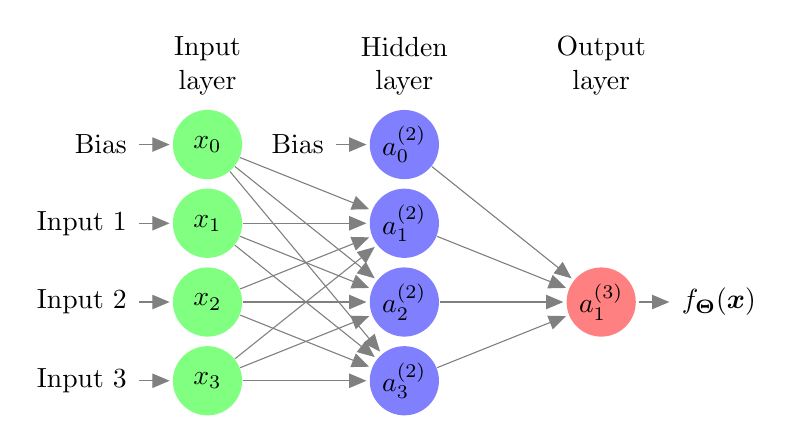
\begin{tikzpicture}[shorten >=1pt,->,draw=black!50, node distance=2.5cm]
    \tikzstyle{every pin edge}=[<-,shorten <=1pt]
    \tikzstyle{neuron}=[circle,fill=black!25,minimum size=25pt,inner sep=0pt]
    \tikzstyle{input neuron}=[neuron, fill=green!50];
    \tikzstyle{output neuron}=[neuron, fill=red!50];
    \tikzstyle{hidden neuron}=[neuron, fill=blue!50];
    \tikzstyle{annot} = [text width=4em, text centered]
    
	\node[input neuron, pin=left:Bias] (I-0) at (0,0) {$x_0$};
    % Draw the input layer nodes
    \foreach \name / \y in {1,...,3}
    % This is the same as writing \foreach \name / \y in {1/1,2/2,3/3,4/4}
        \node[input neuron, pin=left:Input \y] (I-\name) at (0,-\y) {$x_\y$};

 \path[yshift=0cm]
            node[hidden neuron, pin=left:Bias] (H-0) at (2.5cm,0) {$a^{(2)}_0$};
    % Draw the hidden layer nodes
    \foreach \name / \y in {1,...,3}
        \path[yshift=0cm]
            node[hidden neuron] (H-\name) at (2.5cm,-\y) {$a^{(2)}_\y$};

    % Draw the output layer node
	\path[yshift=1cm]    
    node[output neuron,pin={[pin edge={->}]right:$f_{\bm{\Theta}}(\bm{x})$}, right of=H-2] (O) {$a_1^{(3)}$};

    % Connect every node in the input layer with every node in the
    % hidden layer.
    \foreach \source in {0,...,3}
        \foreach \dest in {1,...,3}
            \path (I-\source) edge (H-\dest);

    % Connect every node in the hidden layer with the output layer
    \foreach \source in {0,...,3}
        \path (H-\source) edge (O);

    % Annotate the layers
    \node[annot,above of=H-0, node distance=1cm] (hl) {Hidden layer};
    \node[annot,left of=hl] {Input layer};
    \node[annot,right of=hl] {Output layer};
\end{tikzpicture}
\caption{\small Example Neural Network Structure with 3 external inputs, 1 hidden layer with 3 nodes, 1 bias node per non-output layer and 1 output node. The variable inside each node denotes it's output as calculated in Section 2.2: the output of node $i$ in layer $j$ is denoted as $a_i^{(j)}$. $\bm{\Theta}$ denotes the weights of the network.}
\end{figure}
\newpage
\begin{example}
In this example, we follow Figure 2.3, describing a neural network with 3 inputs, 1 hidden layer with 3 nodes and 1 output node. We denote the activation function as $g$, the output of node $i$ in layer $j$ as $a^{(j)}_i$, and the matrix of weights from layer $j$ to $j+1$ as $\Theta^{(j)}$. The activation function may vary with each node, but typically each layer uses the same activation function for each node. We also use the subscript $\Theta^{(j)}_{m,n}$ where $m$ is the row of the matrix corresponding to the node $m$ in layer $j+1$, and $n$ is the column of the matrix relating to node $n$ in layer $j$.

Denoting the weights outputting to unit $i$ in layer $j+1$ as $\bm{\theta}^{(j)}_i$, we have the following relation between the node weights as described in Section 2.2 and these weight matrices: $\bm{\theta}^{(j)}_i = [\Theta_{i,0}^{(j)}\quad \Theta_{i,1}^{(j)}\cdots \Theta_{i,k}^{(j)}]^\top$, where $k+1$ is the number of inputs.

Individually, the outputs in the hidden nodes and the output node are:
\[x_0=1,\qquad a_0^{(2)}=1\]
\[a_1^{(2)}=g(\Theta^{(1)}_{1,0}x_0+\Theta^{(1)}_{1,1}x_1+\Theta^{(1)}_{1,2}x_2+\Theta^{(1)}_{1,3}x_3)=g((\bm{\theta}^{(1)}_1)^\intercal\bm{x})\]
\[a_2^{(2)}=g(\Theta^{(1)}_{2,0}x_0+\Theta^{(1)}_{2,1}x_1+\Theta^{(1)}_{2,2}x_2+\Theta^{(1)}_{2,3}x_3)=g((\bm{\theta}^{(1)}_2)^\top\bm{x})\]
\[a_3^{(2)}=g(\Theta^{(1)}_{3,0}x_0+\Theta^{(1)}_{3,1}x_1+\Theta^{(1)}_{3,2}x_2+\Theta^{(1)}_{3,3}x_3)=g((\bm{\theta}^{(1)}_3)^\top\bm{x})\]
\[f_\Theta(\bm{x})=a_1^{(3)}=g(\Theta^{(2)}_{1,0}a_0^{(2)}+\Theta^{(2)}_{1,1}a_1^{(2)}+\Theta^{(2)}_{1,2}a_2^{(2)}+\Theta^{(2)}_{1,3}a_3^{(2)})=g((\bm{\theta}^{(2)}_1)^\top\bm{a}^{(2)}),\]
where $\bm{a}^{(2)}=[a_0^{(2)}\quad a_1^{(2)}\quad a_2^{(2)}\quad a_3^{(3)}]^\top$.
%An even simpler notation is:
%\[a_0^{(2)}=1\]
%\[[a_1^{(2)}\quad a_2^{(2)}\quad a_3^{(2)}]=g((\Theta^{(1)})^\top\bm{x})\]
%\[f_{\bm{\Theta}} (\bm{x})=\bm{a}^{(3)}=g((\Theta^{(2)})^\top\bm{a}^{(2)}).\]
\end{example}
\newpage
%\section{Bias-per-node Representation}
%The use of a bias node leads to a minor programming inconvenience: the number of inputs in each layer is one more than the number of outputs of each node in the preceding layer. To make these values consistent, the bias node is often replaced with an intercept term added to the weighted input of a node before it passes through the activation function\citep{DeepLearning}. These intercept terms are optimized alongside the weights. In either case, the bias takes the form of a scalar added to the weighted inputs, which can be optimized. There is no practical difference between these two notations: the sum of intercept terms in a layer is equivalent to the weight corresponding to a bias node for the layer. Figures 2.4 and 2.5 below illustrate this concept, repeating the example of an individual node with three inputs, but with an individual intercept $b_i$ per node.\\
%\begin{figure}[h]
%\begin{tikzpicture}[shorten >=1pt,->,draw=black!50, node distance=2.5cm]
  %  \tikzstyle{every pin edge}=[<-,shorten <=1pt]
  %  \tikzstyle{neuron}=[circle,fill=black!25,minimum size=50pt,inner sep=0pt]
  %  \tikzstyle{input neuron}=[neuron, fill=green!50];
  %  \tikzstyle{output neuron}=[neuron, fill=red!50];
  %  \tikzstyle{hidden neuron}=[neuron, fill=blue!50];
  %  \tikzstyle{annot} = [text width=4em, text centered]

    % Draw the input layer nodes
 %   \foreach \name / \y in {0,...,3}
    % This is the same as writing \foreach \name / \y in {1/1,2/2,3/3,4/4}
      %  \node[input neuron, pin=left:Bias $x_0$] (I-0) at (0,-0) {$\theta_0 x_0$};
	%\foreach \name / \y in {1,...,3}
    % This is the same as writing \foreach \name / \y in {1/1,2/2,3/3,4/4}
     %   \node[input neuron, pin=left:Input $x_{\y}$] (I-\name) at (0,-2*\y) {$\theta_{\y}x_\y+b_\y$};
    % Draw the hidden layer nodes
    %\foreach \name / \y in {1,...,5}
     %   \path[yshift=0.5cm]
      %      node[hidden neuron] (H-\name) at (\layersep,-\y cm) {};

    % Draw the output layer node
    %\node[output neuron,pin={[pin edge={->}]right:$h_{\bm{\theta}}(x)$}, right of=I-2, node distance=4cm] (O) {$g\left(\sum\limits^3_{i=1}(\theta_ix_i+b_i)\right)$};

    % Connect every node in the input layer with every node in the
    % hidden layer.
   % \foreach \source in {1,...,4}
    %    \foreach \dest in {1,...,5}
     %       \path (I-\source) edge (H-\dest);

    % Connect every node in the hidden layer with the output layer
%    \foreach \source in {1,...,3}
%        \path (I-\source) edge (O);
%
%    % Annotate the layers
%%    \node[annot,above of=H-1, node distance=1cm] (hl) {Hidden layer};
%    \node[annot,above of=I-1, node distance=1.4cm](il) {Weighted Inputs};
%    \node[annot,right of=il, node distance=4cm] {Activation Function};
%\end{tikzpicture}
%%\caption{Individual Node Structure: Bias-per-node Representation}
%\end{figure}
%\begin{figure}[h]
%\begin{tikzpicture}[shorten >=1pt,->,draw=black!50, node distance=2.5cm]
%    \tikzstyle{every pin edge}=[<-,shorten <=1pt]
%    \tikzstyle{neuron}=[circle,fill=black!25,minimum size=25pt,inner sep=0pt]
%    \tikzstyle{input neuron}=[neuron, fill=green!50];
%    \tikzstyle{output neuron}=[neuron, fill=red!50];
%    \tikzstyle{hidden neuron}=[neuron, fill=blue!50];
%    \tikzstyle{annot} = [text width=4em, text centered]
%    
%	%\node[input neuron, pin=left:Bias] (I-0) at (0,0) {$x_0$};
%    % Draw the input layer nodes
%    \foreach \name / \y in {1,...,3}
%    % This is the same as writing \foreach \name / \y in {1/1,2/2,3/3,4/4}
%        \node[input neuron, pin=left:Input \y] (I-\name) at (0,-\y) {$x_\y$};
%
% %\path[yshift=0cm]
%  %          node[hidden neuron, pin=left:Bias] (H-0) at (2.5cm,0) {$a^{(2)}_0$};
%    % Draw the hidden layer nodes
%    \foreach \name / \y in {1,...,3}
%        \path[yshift=0cm]
%            node[hidden neuron] (H-\name) at (2.5cm,-\y) {$a^{(2)}_\y$};
%
%    % Draw the output layer node
%	\path[yshift=1cm]    
%    node[output neuron,pin={[pin edge={->}]right:$f_\Theta(x)$}, right of=H-2] (O) {$a_1^{(3)}$};
%
%    % Connect every node in the input layer with every node in the
%    % hidden layer.
%    \foreach \source in {1,...,3}
%        \foreach \dest in {1,...,3}
%            \path (I-\source) edge (H-\dest);
%
%    % Connect every node in the hidden layer with the output layer
%    \foreach \source in {1,...,3}
%        \path (H-\source) edge (O);
%
%    % Annotate the layers
%    \node[annot,above of=H-1, node distance=1cm] (hl) {Hidden layer};
%    \node[annot,left of=hl] {Input layer};
%    \node[annot,right of=hl] {Output layer};
%\end{tikzpicture}
%\caption{Neural Network Structure: Bias-per-node Representation}
%\end{figure}
%\newpage
%Note here that $\sum^3_{i=1}b_i=\theta_0x_0$. The representation of the simple neural network example in Example 2.3.1 becomes:
%\[a_1^{(2)}=g(\Theta^{(1)}_{1,1}x_1+b^{(1)}_1+\Theta^{(1)}_{1,2}x_2+b^{(1)}_2+\Theta^{(1)}_{1,3}x_3+b^{(1)}_3)\]
%\[a_2^{(2)}=g(\Theta^{(1)}_{2,1}x_1+b^{(1)}_1+\Theta^{(1)}_{2,2}x_2+b^{(1)}_2+\Theta^{(1)}_{2,3}x_3+b^{(1)}_3)\]
%\[a_3^{(2)}=g(\Theta^{(1)}_{3,1}x_1+b^{(1)}_1+\Theta^{(1)}_{3,2}x_2+b^{(1)}_2+\Theta^{(1)}_{3,3}x_3+b^{(1)}_3)\]
%\[f_{\bm{\Theta}}(\bm{x})=a_1^{(3)}=g(\Theta^{(2)}_{1,1}a_1^{(2)}+b^{(2)}_1+\Theta^{(2)}_{1,2}a_2^{(2)}+b^{(2)}_2+\Theta^{(2)}_{1,3}a_3^{(2)}+b^{(2)}_3)\]
%or in vectorized notation,
%\[\bm{a}^{(2)}=g((\Theta^{(1)})^\top\bm{x})\]
%\[f_{\bm{\Theta}}(\bm{x})=\bm{a}^{(3)}=g((\Theta^{(2)})^\top\bm{a}^{(2)})\]
%\section{Choice of Activation Function}
%In this section we describe the activation functions commonly used in the different layers of a neural network. Recall in section 2.2 the four most common activation functions are:
%\begin{itemize}
%\item The rectified linear unit or ReLU activation function $g(x)=\max\{0,x\}$ ranging in $[0,\infty)$.
%\item The sigmoid or logistic activation function $g(x)=(1+\exp(-x))^{-1}$ restricted to $(0,1)$.
%\item The hyperbolic tangent function $g(x)=\tanh(x)$ ranging between $(-1,1)$.
%\item The linear activation function $g(x)=x$ ranging in $\R$.
%\end{itemize}
%Rectified linear units are the default choice for the hidden layers for their many advantages \citep{DeepLearning}
%\begin{itemize}
%\item Reduces overfitting: since negative ReLU inputs result in a zero output, on average only half of the units are "active" (non-zero output) when the network is first initialized. The proportion of active units can increase or decrease during training such that overfitting and underfitting is minimized.
%\item Faster computation: a $\max\{0,x\}$ function is computed much faster than a function that uses $\exp$ or $\tanh$.
%\item Easier and more consistent training: weight training in a neural network (discussed in Section 2.6) uses the gradient of overall node function, which is influenced by the activation function. The rectified linear unit has a consistent gradient $\theta$ or $0$ resulting in consistent training, as opposed to more complex units. Since the ReLU function is not differentiable at 0, the derivative $g'(0)$ is usually set to 0.
%\end{itemize}
%Since the input layer has no activation function, it can be described as having a linear activation function.\\
%For the output layer, the activation function with the most reasonable output range is used. This depends on what the network is being used for. For example, in classification, the network assigns a probability to each case, so a sigmoid activation function would be most reasonable, as it ranges between 0 and 1. On the other hand, a rectified linear unit would be used for regression of a non-negative quantity such as price or time.
\section{Weight Initialisation}
Proper initialisation of the weights $\bm{\Theta}_i$ is ideal to improve network training (discussed in Sections 2.6 and 2.7), as if the weights are too low, then the nodal outputs will continually decrease through the layers and become very small, resulting in a significant loss value which requires many iterations of training to fix. A similar scenario occurs when the initial weights are too high \citep{bishop}. In this section we discuss Xavier Initialization \citep{xavier}, a common initialisation method used in deep learning which aims to keep the signal variance constant throughout the network. To derive the initialization algorithm, first consider a single node with $n+1$ inputs, and let $z$ denote the weighted sum of the inputs $\bm{\theta}^\top\bm{x}$ before it is passed through the activation function. This is written as
\[z=\theta_0+\sum^n_{i=1}\theta_ix_i.\]
Here, $\theta_0$ is constant with respect to the external input, so $\Var(\theta_0)=0$. Now without any prior knowledge of the inputs and weights, we assume that they are independent and have 0 mean. We can then find the variance of the other terms by using the formula for the product of independent variables\citep{goodman}:
\begin{align*}
Var(\theta_ix_i)&=\E[x_i]^2\Var(\theta_i)+\E[\theta_i]^2\Var(x_i)+\Var(\theta_i)\Var(x_i)\\
&=\Var(\theta_i)\Var(x_i).
\end{align*}
Assuming that the weights and inputs are also identically distributed, we have
\[\Var(z)=n\Var(\theta_i)\Var(x_i).\]
Since we want constant variance of the signals throughout the network, we set $\Var(z)=\Var(x_i)$ and the result follows:
\[\Var(\theta_i)=\frac1n.\]
However, this result only considers forward propagation of the signal. A variation of this result accounts for back propagation by averaging the number of input and output nodes:
\[\Var(\theta_i)=\frac{2}{n_{in}+n_{out}}.\]
Thus, to enforce constant signal variance throughout the network, the ideal initialization of weights is to sample from a distribution, typically uniform or Gaussian, with $0$ mean and $\frac{2}{n_{in}+n_{out}}$ variance:
\[\theta_i\sim U\left(-\sqrt{\frac{6}{n_{in}+n_{out}}},\sqrt{\frac{6}{n_{in}+n_{out}}}\right)\]
or
\[\theta_i\sim N\left(0,\frac{2}{n_{in}+n_{out}}\right).\]
\section{Optimisation}
The goal of optimising the network is to train the weights of the network such that a loss function, which we will denote as $L$, is minimized. A common loss function is the squared error between the batch of network outputs and the actual results, so our objective function would be:
\[\min_\Theta L(\Theta)=\frac12 (\bm{y}-\bm{f}_\Theta(\bm{x}))^\top(\bm{y}-\bm{f}_\Theta(\bm{x})).\]
The $\frac12$ factor is included to eliminate the factor of 2 in the derivative, simplifying the derivations. The derivative is multiplied by an arbitrary training rate during optimization so there is no significant impact of including that term \citep{DeepLearning}.

Back-propagation (Section 2.8) is used to calculate the partial derivative of the loss function with respect to each individual weight. These partial derivatives are used in the gradient-based optimisation of the weights. There are many variations of neural network optimisation algorithms, but they are mostly based off gradient descent, which we will cover in this section \citep{optimneural}.
\begin{definition}
At point $\bm{x}^{(n)}$, $\bm{s}^{(n)}$ is a descent direction if $\nabla f\left(\bm{x}^{(n)}\right)^\top \bm{s}^{(n)}<0$.
\end{definition}
Gradient descent \citep{optim} is an algorithm used to find the minimizer $\bm{x}^*$ of a function $f$ by iterating on an arbitrary point $\bm{x}^{(n)}$, taking steps proportional to a descent direction $\bm{s}^{(n)}$:
\[\bm{x}^{(n+1)}=\bm{x}^{(n)}+\alpha \bm{s}^{(n)},\qquad \alpha>0.\]
%\begin{figure}
%\centering
%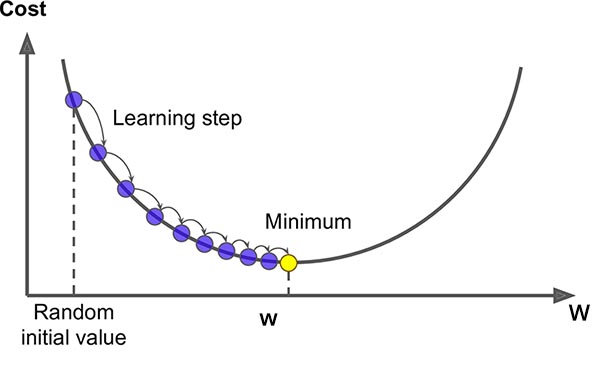
\includegraphics[scale=2]{gradientdescent.jpg}
%\caption{Gradient Descent}
%\end{figure}
\begin{proposition} If $\bm{s}^{(n)}$ is a descent direction for $x^{(n)}$, then for small $\alpha>0$,
\[f(\bm{x}^{(n)}+\alpha \bm{s}^{(n)})<f(\bm{x}^{(n)}).\]
\begin{proof}
First we show that
\[\frac{d}{d\alpha}f(\bm{x}^{(n)}+\alpha \bm{s}^{(n)})=\nabla f(\bm{x}^{(n)}+\alpha \bm{s}^{(n)})^\top \bm{s}^{(n)},\]
where $\bm{x}^{(n)}=[x_1^{(n)},\dots,x_k^{(n)}]^\top$ and $\bm{s}^{(k)}=[s_1^{(n)},\dots,s_k^{(n)}]^\top$.\\
Let
\[x_i^{(n)}(\alpha)=x_i^{(n)}+\alpha s_i^{(n)},\quad i=1,\dots,n,\]
so that $\bm{x}^{(n)}+\alpha \bm{s}^{(n)}=[x_1^{(n)}(\alpha),\dots,x_k^{(n)}(\alpha)]^\top$.
We have
\begin{align*}
\frac{d}{d\alpha}f(\bm{x}^{(n)}+\alpha\bm{s}^{(n)})&= \frac{d}{d\alpha}f(x_1^{(n)},\dots,x_k^{(n)}(\alpha))\\
&= \sum^k_{i=1}\frac{\partial f(\bm{x})}{\partial x_i}|_{\bm{x}=\bm{x}^{(n)}+\alpha \bm{s}^{(n)}}\frac{d(x_i^{(n)}(\alpha))}{d\alpha}\\
&=\sum_{i=1}^k\frac{\partial f(\bm{x})}{\partial x_i}|_{\bm{x}=\bm{x}^{(n)}+\alpha \bm{s}^{(n)}}\bm{s}_i^{(n)}\\
%\frac{\partial f(\bm{x})}{\partial x_1}|_{\bm{x}=\bm{x}^{(n)}+\alpha \bm{s}^{(n)}}\bm{s}_1^{(n)}+\dots+\frac{\partial f(\bm{x})}{\partial x_n}|_{\bm{x}=\bm{x}^{(n)}+\alpha \bm{s}^{(n)}}\bm{s}_k^{(n)}\\
&=\nabla f(\bm{x}^{(n)}+\alpha \bm{s}^{(n)})^\top \bm{s}^{(n)}
\end{align*}
Setting $\alpha=0$ and using Definition 2.7.1,
\[\frac{d}{d\alpha}f(\bm{x}^{(n)}+\alpha\bm{s}^{(n)})|_{\alpha=0}=\nabla f(\bm{x}^{(n)})^\top \bm{s}^{(n)}<0.\]
Therefore for small $\alpha>0$,
\[f(x^{(n)}+\alpha s^{(n)})<f(x^{(n)}).\]
\end{proof}
\end{proposition}
A common choice of descent direction is the negative of the gradient, that is, $-\nabla f(\bm{x}^{(n)})$, leading to the method of steepest descent. It is clearly a descent direction as $-\nabla f(\bm{x}^{(n)})^\top\nabla f(\bm{x}^{(n)})=-\|\nabla f(\bm{x}^{(n)})\|^2<0$, where $\|\cdot\|$ denotes the Euclidean norm.

By nature, gradient descent is guaranteed to converge to a local minimum, which is problematic if the function has local minima which differ from the global minima. This is not an issue in this thesis, as all the loss functions we use are convex, so any local minima are also global minima. Those interested in global optimization can refer to ``Deterministic Global Optimization" by \citet{floudas}. When training a neural network on a non-convex loss function there are currently no commonly used methods of guaranteeing a global minimum, but the path may escape from a local minimum if randomness is introduced to the training process. This can be accomplished by stochastic gradient descent.

Typically, the entire batch of data is used in each iteration to calculate the loss function and gradient values required for gradient descent. This method of batch gradient descent is very slow for large datasets. Stochastic gradient descent is defined by the use of only one observation per iteration, so the latent randomness associated with each observation effectively leads to noise added to each step, but the optimization is much faster. In practice, a compromise between stochastic and batch gradient descent is typically used; mini-batch gradient descent involves using several observations per iteration, leading to a reduction in the gradient variance \citep{batch, optimneural}. The size of the batch depends on the size and nature of the data set. For small data sets, the batch would typically be the entire data set as this would computationally feasible. On the other hand, online data is stochastic in nature and the data set is generally very large, so a small batch size would be used \citep{bengio}.

Gradient descent convergence can be improved by using an adaptive learning rate, adjusting $\alpha$ over the iterations, as a low learning rate in the process will make convergence slow, whilst a high learning rate can cause the algorithm to oscillate around the minima \citep{optimneural}.

In this thesis, we use the Adam algorithm, which incorporates these two concepts to form an effective optimization algorithm that is commonly applied to neural networks. It uses the first and second moments of the gradient decay rate to adapt the weight training rate. More details can be found in Adam: A Method for Stochastic Optimization by Kingma, Ba \citep{adam}.
\section{Back-Propagation}
In the back-propagation algorithm, the goal is to find the partial derivative of the loss function with respect to the individual weights \[\frac{\partial}{\partial\Theta_{m,n}^{(j)}}L(\Theta),\]
so that gradient descent can be performed to optimize the weights \citep{backprop}. For each training sample $(\bm{x}^{(I)},\bm{y}^{(I)})$, $I=1,\dots,N$, the input signal is propagated forward throughout the network to calculate $\bm{a}^{(j)}$ for $j=2,\dots,J$, where $J$ is the total number of layers. The difference between the network output and the ideal result is calculated with 
\[\bm{\delta}^{(J)}=\bm{a}^{(J)}-\bm{y}^{(I)},\] 
and this error is propagated backwards through the network to find $\bm{\delta}^{(J-1)},\dots,\bm{\delta}^{(2)}$ by using the formula 
\[\bm{\delta}^{(j)}=((\Theta^{(j)})^\top \bm{\delta}^{(j+1)}).~*g'(\Theta^{(j)^\top} \bm{a}^{(j)}),\] 
where $.~*$ denotes element-wise multiplication and $g'$ is the derivative of the activation function. In this case, $g'$ takes in the sum of its weighted inputs, and as an example, the sigmoid activation function has the derivative $g'(\Theta^{(j)^\top} \bm{a}^{(j)})=\bm{a}^{(j)}.~*(1-\bm{a}^{(j)})$. Note that $\bm{\delta}^{(1)}$ does not need to be calculated as the input layer is not weighted. \\
The errors for each layer are multiplied by each of the preceding layer's activation outputs to form the estimated partial derivative for the training sample. This result is added to an accumulator matrix, so that the average partial derivative from all the training samples can be computed:
\[\Delta^{(j)}_{m,n}:=\Delta^{(j)}_{m,n}+a_n^{(j)}\delta_m^{(j+1)}\]
or in matrix-vector form.
\[\Delta^{(j)}:=\Delta^{(j)}+\bm{\delta}^{(j+1)}(\bm{a}^{(j)})^\top.\]
Finally, we divide the accumulator matrix entries by the number of training samples to find the average partial derivative of the cost function with respect to the weights:
\[\frac{\partial}{\partial \Theta^{(j)}_{m,n}}L(\Theta)=\frac1N \Delta_{m,n}^{(j)}.\]
When $n\neq0$ (i.e. not considering the bias node), we can optionally add a regularizer term $\lambda > 0$ which decreases the magnitude of the weights, reducing overfitting \citep{DeepLearning}
\[\frac{\partial}{\partial \Theta^{(j)}_{m,n}}L(\Theta)=\frac1N (\Delta_{m,n}^{(j)}+\lambda \Theta_{m,n}^{(j)}).\]
There is no significant change when the bias node is regularized.\\
Pseudocode for back-propagation is shown in Algorithm 1 below.\\
\begin{algorithm}
\caption{Back-Propagation Algorithm}
\KwData{Training Data $\{(\bm{x}^{(1)},\bm{y}^{(1)}),\dots ,(\bm{x}^{(N)},\bm{y}^{(N)})\}$, Regularizer Term $\lambda$}
\KwResult{Cost Function Partial Derivatives $\frac{\partial}{\partial\Theta^{(j)}_{m,n}}L(\Theta)$}
\BlankLine
\Begin{Initialize weights $\Theta$ using Xavier Initialisation\;
Set $\Delta^{(j)}_{m,n}=0 \quad \forall j,m,n$\;
\For{$I=1$ \KwTo $N$}{
Set $\bm{a}^{(1)}=\bm{x}^{(I)}$\;
\For{$j=2$ \KwTo $J$}{
Set $\bm{a}^{(j)}=\Theta^{(j-1)^\top}\bm{a}^{(j-1)}$\;}
Set $\bm{\delta}^{(J)}=\bm{a}^{(J)}-\bm{y}^{(I)}$\;
\For{$j=J-1$ \KwTo $2$}{
Set $\bm{\delta}^{(j)}=((\Theta^{(j)})^\top \bm{\delta}^{(j+1)}).*g'(\Theta^{(j)^\top}\bm{a}^{(j)})$\;
}
\For{$j=1$ \KwTo $J-1$}{
Set $\Delta^{(j)}=\Delta^{(j)}+\bm{\delta}^{(j+1)}(\bm{a}^{(j)})^\top$\;
}}
\For{all $j,m,n$}{
\eIf{$n=0$}{Set $\frac{\partial}{\partial\Theta^{(j)}_{m,n}}L(\Theta)=\frac1N \Delta^{(j)}_{m,n}$\;
}{Set $\frac{\partial}{\partial\Theta^{(j)}_{m,n}}L(\Theta)=\frac1N (\Delta^{(j)}_{m,n}+\lambda\Theta^{(j)}_{m,n})$\;}}}
\end{algorithm}
\chapter{Variational Inference}
In this chapter, we explain variational inference, a method that uses a specific functional form to approximate posterior distributions in the context of Bayesian statistics. These are denoted as `variational distributions', from the use of variational calculus to derive certain expressions. We first describe the Bayesian framework and problems associated with computational intractability. We then explain, with examples, two types of variational inference: mean-field variational inference and amortized inference. Finally, the chapter is concluded with a description of issues that arise when one or more of the prior or likelihood distributions are implicit, that is, samples can be readily drawn from them but the density function is difficult to numerically evaluate.
\section{Context}
A fundamental problem in Bayesian statistics is to evaluate, or estimate posterior densities to perform analysis on unknown parameters \citep{gelman}. Consider the set of latent and known variables $\bm{z}=(z_1,\dots,z_M)\in \R^M$ and $\bm{x}=(x_1,\dots,x_N)\in \R^N$, respectively, with joint density $p(\bm{z},\bm{x})$. The posterior density $p(\bm{z}|\bm{x})$ is the distribution of the latent parameters $z_1,\dots,z_M$ conditioned on the known variables $\bm{x}$. Applying Bayes' theorem, it can be written as:
\begin{equation*}
p(\bm{z}|\bm{x})=\frac{p(\bm{z},\bm{x})}{p(\bm{x})}= \frac{p(\bm{z})p(\bm{x}|\bm{z})}{\int_\R p(\bm{z},\bm{x})d\bm{z}},
\end{equation*}
where
\begin{itemize}
\item $p(\bm{z})$ is the prior distribution: the initial distribution of $\bm{z}$ before the data $\bm{x}$ is observed. This can be initialised to represent our subjective beliefs, or it can be an uninformative prior that implies objectivity.
\item $p(\bm{x}|\bm{z})$ is the likelihood: the distribution of data $\bm{x}$ conditioned on the parameters $\bm{z}$.
\item $p(\bm{x})=\int_\mathcal{z}p(\bm{z},\bm{x})d\bm{z}$ is the marginal likelihood, or the evidence: the density of the data averaged across all possible parameter values.
\end{itemize}
In simple cases, the posterior can typically be calculated algebraically by using the proportionality $p(\bm{z}|\bm{x})\propto p(\bm{z})p(\bm{x|z})$ and normalising over the constant $p(\bm{x})$. As the model becomes more complex, the calculations required can be extremely difficult, so
% the evidence integral $p(\bm{x})=\int_\mathbcal{z}p(\bm{z},\bm{x})d\bm{z}$ is computationally intractable, then we are unable to evaluate the posterior density. 
traditional MCMC (Markov Chain Monte Carlo) methods overcome this obstacle by sampling from a Markov chain that converges to the stationary distribution $p(\bm{z}|\bm{x})$. However, these methods tend to have slow convergence for large datasets or high dimensional data. When faced with these issues or when desiring a faster computation, one may instead apply variational inference, an alternative approach to density estimation. Variational inference methods can be much faster than MCMC as they replace sampling with optimisation, but they are known to underestimate the true posterior variance \citep{blei}.

\section{The KL Divergence}
We first define the f-divergence: a measure of how much two probability distributions differ.
\begin{definition}
The f-divergence of continuous probability distribution $Q$ from $P$ is
\[D_f(P\|Q)=\mathbb{E}_{p(u)}\left[f\left(\frac{q(u)}{p(u)}\right)\right],\]
where $f$ is a convex function such that $f(1)=0$.
\end{definition}
When $f(u)=-\log u$, we have the KL (Kullback-Leibler) divergence \citep{KL}, a type of f-divergence that is commonly used in variational inference \citep{blei}.
\begin{definition}
The KL divergence is the expected logarithmic difference between two distributions $P$ and $Q$ with respect to $P$:
\begin{equation*}
KL(p(x)\|q(x))=\int_{-\infty}^\infty p(x)\log \left(\frac{p(x)}{q(x)}\right)dx=\mathbb{E}_{p(x)}\left[\log\left(\frac{p(x)}{q(x)}\right)\right].
\end{equation*}
\end{definition}
\begin{remark}
The KL divergence is not symmetric:
\begin{equation*}
KL(p(x)||q(x))\neq KL(q(x)||p(x))\text{ for }p(x)\neq q(x).
\end{equation*}
\end{remark}
In variational inference, $KL(p(x)\|q(x))$ is known as the forward KL divergence, whilst $KL(q(x)\|p(x))$ is the reverse KL divergence.
\begin{lemma}
The reverse KL divergence is formulated when $f(u)=u\log u$ in an f-divergence.
\begin{proof}
\begin{align*}
D_{RKL}(P\|Q)&=\mathbb{E}_{p(u)}\left[\frac{q(u)}{p(u)}\log \left(\frac{q(u)}{p(u)}\right)\right]\\
&=\int p(u)\frac{q(u)}{p(u)}\log\left(\frac{q(u)}{p(u)}\right)du\\
&= \int q(u)\log\left(\frac{q(u)}{p(u)}\right)du\\
&= \mathbb{E}_q\left[\log \left(\frac{q(u)}{p(u)}\right)\right]\\
&=KL[q(u)\|p(u)].
\end{align*}
\end{proof}
\end{lemma}
Note that the forward and reverse KL divergences mainly differ in the distribution that is used to take the expectation.
\begin{lemma}\label{lemma:3.2.5}
The KL divergence is non-negative, and it is equal to zero if and only if $p(x)$ and $q(x)$ are equivalent:
\begin{equation*}
KL(q(x)||p(x))\geq 0.
\end{equation*}
We prove this in the case where $P$ and $Q$ are continuous distributions: a similar proof holds when they are discrete.
\begin{proof}
\begin{align*}
KL(p(x)\|q(x))&=\int_{-\infty}^\infty p(x)\log \left(\frac{p(x)}{q(x)}\right)dx\\
&=-\int_{-\infty}^\infty p(x)\log \left(\frac{q(x)}{p(x)}\right)dx\\
&\geq -\int_{-\infty}^\infty p(x) \left(\frac{q(x)}{p(x)}-1\right)dx\\
&=-\int_{-\infty}^\infty q(x)dx + \int_{-\infty}^\infty p(x)dx\\
&=0
\end{align*}
In the third line we use $-\log x \geq -(x-1)$ for all $x>0$ with equality if and only if $x=1$, therefore $KL(q(x)\|p(x))=0$ if and only if $q(x)=p(x)$. The last line is due to $p(x)$ and $q(x)$ being probability densities.
\end{proof}
\end{lemma}
\section{Introduction to Variational Inference}
Variational inference approximates the true posterior distribution $p(\bm{z}|\bm{x})$ with a different distribution $q(\bm{z})$, taken from a tractable family of approximate distributions $\mathcal{Q}$, and then minimizes the f-divergence between the two distributions in an optimization problem:
\begin{equation}\label{eqn:3.3.1}
q^*(\bm{z})=\argmin_{q(\bm{z})\in \mathcal{Q}}D_f(q(\bm{z})\|p(\bm{z}|\bm{x})),
\end{equation} where $D_f$ denotes an f-divergence \citep{blei}. This produces an analytic approximation to the posterior density. The most common f-divergence used in variational inference is the reverse KL divergence, used instead of the forward KL divergence as we are unable to sample from our true posterior $p(z|x)$, and because it leads to an expectation maximization algorithm as opposed to an expectation propagation algorithm. \autoref{eqn:3.3.1} can therefore be written as:
\begin{equation}\label{3.3.2}
q^*(\bm{z})=\argmin_{q(\bm{z})\in \mathcal{Q}}KL(q(\bm{z})\|p(\bm{z}|\bm{x})).
\end{equation}
From Lemma 3.2.5, it is evident that $KL(q(\bm{z})\|p(\bm{z}|\bm{x}))$ attains a minimal value of $0$ when $q(\bm{z})=p(\bm{z}|\bm{x})$.\\
There is an issue with solving equation (3.3.2) directly: we cannot evaluate the reverse KL divergence as $p(\bm{z}|\bm{x})$ is unknown. Instead, we rearrange the terms of equation 3.3.2 to formulate a tractable expression that can be optimized.
\section{Derivation of the ELBO}
In this section, we formulate the evidence lower bound (ELBO) of our posterior inference problem. Maximisation of this term is equivalent to solving equation (3.3.2). We begin by applying Bayes' law to the problem and expanding the terms:
\begin{align*}
q^*(\bm{z})&=\argmin_{q(\bm{z})\in \mathcal{Q}}KL(q(\bm{z})\|p(\bm{z}|\bm{x}))\\
&= \argmin_{q(\bm{z})\in \mathcal{Q}} \mathbb{E}_{q(\bm{z})}[\log q(\bm{z})-\log p(\bm{z}|\bm{x})]\\
&= \argmin_{q(\bm{z})\in \mathcal{Q}} \mathbb{E}_{q(\bm{z})}\left[\log q(\bm{z})-\log\frac{p(\bm{x}|\bm{z})p(\bm{z})}{p(\bm{x})}\right]\\
&= \argmin_{q(\bm{z})\in \mathcal{Q}} \left(\mathbb{E}_{q(\bm{z})}[\log q(\bm{z})-\log p(\bm{x}|\bm{z})-\log p(\bm{z})]+\log p(\bm{x})\right).
\end{align*}
Note in the last line $\mathbb{E}_{q(\bm{z})}[p(\bm{x})]=p(\bm{x})$ as it is not dependent on $q(\bm{z})$. Since our issues with equation (3.3.2) result from the intractability of $p(\bm{x})$, we rearrange the KL divergence expression as follows:
\begin{align}
KL(q(\bm{z})\|p(\bm{z}|\bm{x}))&=\mathbb{E}_{q(\bm{z})}[\log q(\bm{z})-\log p(\bm{x}|\bm{z})-\log p(\bm{z})]+\log p(\bm{x}) \nonumber \\
\log p(\bm{x})-KL(q(\bm{z})\|p(\bm{z}|\bm{x}))&=-\mathbb{E}_{q(\bm{z})}[\log q(\bm{z})-\log p(\bm{x}|\bm{z})-\log p(\bm{z})]\nonumber \\
&=\mathbb{E}_{q(\bm{z})}[\log p(\bm{x}|\bm{z})]-\mathbb{E}_{q(\bm{z})}[\log q(\bm{z})-\log p(\bm{z})]\nonumber \\
&=\mathbb{E}_{q(\bm{z})}[\log p(\bm{x}|\bm{z})]-KL(q(\bm{z})\|p(\bm{z}))\\
\log p(\bm{x})&\geq \mathbb{E}_{q(\bm{z})}[\log p(\bm{x}|\bm{z})]-KL(q(\bm{z})\|p(\bm{z})).
\end{align}
We refer to $\log p(\bm{x})-KL(q(\bm{z})\|p(\bm{z}|\bm{x}))$ as $ELBO(q)$, as it is equal to the marginal probability of the data subtracted by a constant `error term'. Now our problem of minimizing the KL divergence between $q(\bm{z})$ and $p(\bm{z}|\bm{x})$ is equivalent to maximizing $ELBO(q)$, which is equal to the tractable expression on line (3.4.1). We can therefore rewrite our optimization problem as:
\begin{align}
q^*(\bm{z})&=\argmin_{q(\bm{z})\in \mathcal{Q}}KL(q(\bm{z})\|p(\bm{z}|\textbf{x}))\nonumber\\
&= \argmax_{q(\bm{z})\in \mathcal{Q}} ELBO(q)\nonumber\\
&= \argmax_{q(\bm{z})\in \mathcal{Q}} \left(\mathbb{E}_{q(\bm{z})}[\log p(\bm{x}|\bm{z})]-KL(q(\bm{z})\|p(\bm{z}))\right).
\end{align}
Note from line (3.4.2) that the expression on line (3.4.3) attains a maximum at the marginal likelihood of the dataset $\log p(\bm{x})$, hence we may use the ELBO to construct a model selection criterion\citep{pattern}. However, this criterion may not be reliable as it is a lower bound.
\newpage
\section{Mean-Field Variational Family}
The family of variational distributions $\mathcal{Q}$ is typically a `mean-field variational family', in which the distribution $q(\bm{z})$ factorizes over the latent variables $\{z_i\}^M_{i=1}$, each with an individual set of parameters $\{\phi_i\}^M_{i=1}$ \citep{blei}:
\begin{equation}
q(\bm{z})=\prod^M_{i=1}q_{\phi_i}(z_i).
\end{equation}
The individual factors $q_{\phi_i}(z_i)$ can take any form, but they are assumed to be independent, which simplifies derivations but is less accurate when the true latent variables exhibit dependence. Fixing the forms of the individual factors, we want to choose the parameters $\phi_i$ so that $ELBO(q)$ is maximized. To derive an expression for the optimal factor $q_i^*(z_i)$, we substitute equation (3.5.1) into the $ELBO$, factor out a specific $q_j(z_j)$ and equate the functional derivative of the resulting Lagrangian equation with 0. \\
Firstly, we express $ELBO(q)$ in an integral form as follows:
\begin{align*}
ELBO(q)&= \mathbb{E}_{q(z)}[\log p(\bm{x}|\bm{z})]-KL(q(\bm{z})\|p(\bm{z}))\\
&= \mathbb{E}_{q(x)}[\log p(\bm{x}|\bm{z})+\log p(\bm{z})-\log q(\bm{z})]\\
&= \mathbb{E}_{q(z)}[\log p(\bm{x}, \bm{z})-\log q(\bm{z})]\\
&= \int_{\R^M}q(\bm{z})(\log p(\bm{x},\bm{z})-\log q(\bm{z}))d\bm{z}.
\end{align*}
Substituting $q(\bm{z})=\prod^M_{i=1}q_i(z_i)$ and factoring out $q_j(z_j)$ yields:
\begin{align}
ELBO(q)&= \int_{\R^M}\left[\prod^M_{i=1}q_i(z_i)\right]\left(\log p(\bm{x},\bm{z})-\sum_{i=1}^M\log q_i(z_i)\right)d\bm{z}\nonumber\\
&= \int_{\R}q_j(z_j)\left(\int_{\R^{M-1}}\log p(\bm{x},\bm{z})\prod_{i\neq j}q_i(z_i)d\bm{z}_{-j} \right) dz_j\nonumber\\
&\quad -\int_{\R}q_j(z_j)\left(\int_{\R^{M-1}}\left[\prod_{i\neq j}q_i(z_i)\right]\sum_{i=1}^M \log q_i(z_i)d\bm{z}_{-j}\right)dz_j\nonumber\\
&= \int_{\R}q_j(z_j)\mathbb{E}_{\bm{z}_{-j}}[\log p(\bm{x},\bm{z})]dz_j\nonumber\\
&\quad -\int_{\R}q_j(z_j)\log q_j(z_j)\left(\int_{\R^{M-1}}\prod_{i\neq j}q_i(z_i)dz_{-j}\right) dz_j\nonumber\\
&\quad -\int_{\R}q_j(z_j)\left(\int_{\R^{M-1}}\left[\prod_{i\neq j}q_i(z_i)\right]\sum_{i\neq j}\log q_i(z_i)d{\bm{z}_{-j}}\right)dz_j\nonumber\\
&= \int_\R q_j(z_j)\mathbb{E}_{\bm{z}_{-j}}[\log p(\bm{x},\bm{z})]dz_j-\int_\R q_j(z_j)\log q_j(z_j)dz_j\nonumber\\
&\quad -\int_{\R^{M-1}}\left[\prod_{i\neq j}\log q_i(z_i)\right]\sum_{i\neq j}\log q_i(z_i)d{\bm{z}_{-j}}
\\&= \int_{\R}q_j(z_j)\left(\mathbb{E}_{\mathcal{z}_{-j}}[\log p(\bm{x},\bm{z})]-\log q_j(z_j)\right)dz_j+\text{const}.
\end{align}
The term in line (3.5.2) is a constant with respect to $q_j(z_j)$. We want to maximize $ELBO(q)$, so we formulate the Lagrangian equation with the constraint that $q_i(z_i)$ are probability density functions:
\begin{equation*}
ELBO(q)-\sum^M_{i=1}\lambda_i\int_\R q_i(z_i)dz_i=0,
\end{equation*}
or using our expression for $ELBO(q)$ in line (3.5.3),
\begin{equation}
\int_\R q_j(z_j)\left(\mathbb{E}_{\mathcal{z}_{-j}}[\log p(\bm{x},\bm{z})]-\log q_j(z_j)\right)dz_j-\sum^M_{i=1}\lambda_i\int_\R q_i(z_i)dz_i+\text{const}=0.
\end{equation} 
Using the Euler-Legendre equation, we then take the functional derivative of equation (3.5.4) with respect to $q_j(z_j)$ \citep{pattern}:
\begin{align}
\frac{\partial ELBO(q)}{\partial q_j(z_j)}&= \frac{\partial}{\partial q_j(z_j)}\left[q_j(z_j)\left(\mathbb{E}_{\bm{z}_{-j}}[\log p(\bm{x},\bm{z})]-\log q_j(z_j)\right)-\lambda_jq_j(z_j)\right]\nonumber
\\&= \mathbb{E}_{\bm{z}_{-j}}[\log p(\bm{x},\bm{z})]-\log q_j(z_j)-1-\lambda_j.
\end{align}
Equating expression (3.5.5) to 0 and observing that $1+\lambda_j$ is constant with respect to $z$, we have:
\begin{align}
\log q_j^*(z_j)&= \mathbb{E}_{\bm{z}_{-j}}[\log p(\bm{x},\bm{z})]-\text{const} \nonumber\\
q_j^*(z_j)&=\frac{e^{\mathbb{E}_{\bm{z}_{-j}}[\log p(\bm{x},\bm{z})]}}{\exp{(\text{const})}}\nonumber\\
&= \frac{e^{\mathbb{E}_{\bm{z}_{-j}}[\log p(\bm{x},\bm{z})]}}{\int e^{\mathbb{E}_{\bm{z}_{-j}}[\log p(\bm{x},\bm{z})]}dz_j}.
\end{align}
\newpage
The normalization constant on the denominator of (3.5.6) is derived by observing $q^*_j(z_j)$ as a density. Finally, we derive a simpler expression of $q^*_j(z_j)$ by observing that terms independent of $z_j$ can be treated as a constant:
\begin{align}
q^*_j(z_j)&\propto \exp\left(\mathbb{E}_{\bm{z}_{-j}}[\log p(\bm{x},\bm{z})]\right)\nonumber\\
&\propto \exp\left(\mathbb{E}_{\bm{z}_{-j}}[\log p(z_j|\bm{z}_{-j},\bm{x})]\right).
\end{align}
This expression can be used in an expectation-maximization algorithm, in which the $q^*_j(z_j)$ is evaluated and iterated from $j=1\dots M$ until $ELBO(q)$ converges. We can say this occurs when there is little variation in $ELBO(q)$ over the iterations. This particular algorithm is called coordinate ascent variational inference (CAVI) (Algorithm 2):\\
\\
\begin{algorithm}[H]
\caption{Coordinate Ascent Variational Inference (CAVI)}
\KwData{Dataset $\bm{x}$ and Bayesian Model p($\bm{x},\bm{z}$)}
\KwResult{Variational density $q(\bm{z})=\prod^M_{i=1}q_i(z_i)$}
\BlankLine
\Begin{
Initialize random variational factors $q_j(z_j)$\;
\While{ELBO(q) has not converged}{

	\For{$j=1$ \KwTo $m$}{
	Set $q_j(z_j)\propto \exp(\mathbb{E}_{\bm{z}_{-j}}[\log p(z_j|\bm{z}_{-j},\bm{x})])$\;
	}
	Calculate $ELBO(q)=\mathbb{E}_{q(\bm{z})}[\log p(\bm{z},\bm{x})]-\mathbb{E}_{q(\bm{z})}[\log q(\bm{z})]$\;
}
Return $q(\bm{z})$\;
}
\end{algorithm}
\newpage
\section{Example: Bayesian Mixture of Gaussians}
To illustrate the mean-field variational inference approach, we closely follow the ``Bayesian mixture of Gaussians" example from ``Variational Inference: A Review for Statisticians" by \citet{blei}.\\
Consider the hierarchical model
\begin{align*}
\mu_k&\sim N(0,\sigma^2), &&k=1,\dots,K,\\
c_i&\sim \text{Categorical}\left(1;\frac{1}{K},\dots,\frac{1}{K}\right), &&i=1,\dots,n,\\
x_i|c_i,\bm{\mu}&\sim N(c^\top_i\bm{\mu},1), &&i=1,\dots,n,
\end{align*}
where $\bm{\mu}=(\mu_1,\dots,\mu_K)^\top$.\\
This is a Bayesian mixture of univariate Gaussian random variables with unit variance. In this model, we draw $K$ $\mu_k$ variables from a prior Gaussian distribution $N(0,\sigma^2)$ ($\sigma^2$ is a fixed hyperparameter), forming the vector $\bm{\mu}$. We then generate an indicator vector $c_i$ of length $K$ from a prior categorical distribution. This vector has zeros for every element except for one element, where it is a $1$. Each element has equal probability $1/K$ of being the element that is equal to $1$. The transpose of this $c_i$ is then multiplied by $\bm{\mu}$, essentially choosing one of the $\bm{\mu}$ elements at random. We then draw $x_i$ from the resulting $N(c^\top_i\bm{\mu},1)$.\\
Defining $\bm{c}=(c_1,\dots,c_n)^\top$, our latent variables are $\bm{z}=\{\bm{c},\bm{\mu}\}$. Assuming $n$ samples, our joint density is
\begin{equation}
p(\bm{\mu},\bm{c},\bm{x})=p(\bm{\mu})\prod^n_{i=1}p(c_i)p(x_i|c_i, \bm{\mu}).\end{equation}
%From this, we derive the marginal likelihood
%\begin{align*}
%p(\bm{x})&=\int p(\bm{\mu})\sum_{c_i}\prod^n_{i=1}p(c_i)p(x_i|c_i,\bm{\mu})d\bm{\mu}\\
%&=\int p(\bm{\mu})\prod^n_{i=1}\sum_{c_i}p(c_i)p(x_i|c_i,\bm{\mu})d\bm{\mu}.
%\end{align*}
%This integral is intractable, as the time complexity of evaluating it is $\mathcal{O}(K^n)$, which is exponential in $K$. 
To evaluate the posterior distribution over the latent variables $p(\bm{\mu},\bm{c}|\bm{x})$, we apply variational inference, approximating it with a variational distribution $q(\bm{\mu},\bm{c})$. We will assume this distribution follows the mean-field variational family:
\[q(\bm{\mu},\bm{c})=\prod^K_{k=1}q(\mu_k;m_k,s^2_k)\prod^n_{i=1}q(c_i;\bm{\phi_i}).\]
\newpage
In this distribution, we have $K$ Gaussian factors with mean $m_k$ and variance $s^2_k$, and $n$ categorical factors with index probabilities defined by the vector $\bm{\phi_i}$, such that
\begin{align*}
\mu_k&\sim N(m_k,s^2_k), &&k=1,\dots,K,\\
c_i&\sim \text{Categorical}(\bm{\phi_i}), &&i=1,\dots,n.
\end{align*}
Using this and equation (3.6.1), we can derive the evidence lower bound as a function of the variational parameters $\bm{m}=(m_1,\dots,m_k)^\top$, $\bm{s}^2=(s_1^2,\dots,s_k^2)^\top$ and $\bm{\phi}=[\bm{\phi}_1,\dots,\bm{\phi}_n]^\top$:
\begin{align*}
ELBO(\bm{m},\bm{s}^2,\bm{\phi})&=\mathbb{E}_{p(\textbf{z},\bm{x})}[\log p(\textbf{z},\bm{x})]-\mathbb{E}_{q(\bm{z})}[\log q(\bm{z})]\\
&=\mathbb{E}_{p(\bm{\mu,c},\textbf{x})}[\log p(\bm{\mu,c},\textbf{x})]-\mathbb{E}_{q(\bm{\mu,c})}[\log q(\bm{\mu,c})]\\
&=\sum^K_{i=1}\mathbb{E}_{p(\mu_k)}[\log p(\mu_k); m_k,s^2_k]\\
&\quad +\sum^n_{i=1}\left(\mathbb{E}_{p(c_i)}[\log p(c_i);\bm{\phi}_i]+\mathbb{E}_{p(x_i|c_i,\bm{\mu})}[\log p(x_i|c_i,\bm{\mu});\bm{\phi}_i,\bm{m},\bm{s}^2]\right)\\
&\quad -\sum^K_{k=1}\mathbb{E}_{q(\mu_k;m_k,s^2_k)}[\log q(\mu_k;m_k,s^2_k)]-\sum^n_{i=1}\mathbb{E}_{q(c_i;\bm{\phi}_i)}[\log q(c_i;\bm{\phi}_i)].
\end{align*}
From equation (3.5.7), we derive the optimal categorical factor by only considering terms from the true distribution $p(\cdot)$ dependent on $c_i$:
\begin{equation}
q^*(c_i;\bm{\phi}_i)\propto \exp\left(\log p(c_i)+\mathbb{E}_{p(x_i|c_i,\bm{\mu})}[\log p(x_i|c_i,\bm{\mu});\bm{m},\bm{s}^2]\right).
\end{equation}
Now since $c_i=(c_{i1},\dots,c_{iK})^\top$ is an indicator vector,
\[p(x_i|c_i,\bm{\mu})=\prod^K_{k=1}p(x_i|\mu_k)^{c_{ik}}.\]
We can now evaluate the second term of equation (3.6.2):
\begin{align*}
\mathbb{E}_{p(x_i|c_i,\bm{\mu})}\left([\log p(x_i|c_i,\bm{\mu});\bm{m},\bm{s}^2]\right)&=\sum_{k=1}^K c_{ik}\mathbb{E}_{p(x_i|\mu_k)}[\log p(x_i|\mu_k);m_k,s^2_k]\\
&=\sum_{k=1}^K c_{ik}\mathbb{E}_{x_i}[-(x_i-\mu_k)^2/2;m_k,s^2_k]+\text{const}\\
&=\sum_{k=1}^Kc_{ik}\left(\mathbb{E}_{\mu_k}[\mu_k;m_k,s^2_k]x_i-\mathbb{E}_{\mu_k^2}[\mu^2_k;m_k,s^2_k]/2\right)\\
&\quad +\text{const}.
\end{align*}
In each line, terms constant with respect to $c_{ik}$ have been absorbed into the constant. Our optimal categorical factor becomes
\[q^*(c_i;\bm{\phi}_i)\propto \exp \left(\log p(c_i)+\sum_{k=1}^Kc_{ik}\left(\mathbb{E}_{\mu_k}[\mu_k;m_k,s^2_k]x_i-\mathbb{E}_{\mu^2_k}[\mu^2_k;m_k,s^2_k]/2\right)\right).\]
By proportionality, we then have the variational update
\[\phi_{ik}\propto \exp\left(\mathbb{E}_{\mu_k}[\mu_k;m_k,s^2_k]x_i-\mathbb{E}_{\mu^2_k}[\mu^2_k;m_k,s^2_k]/2\right).\]
Now we find the variational density of the $k$th mixture component, again using equation 3.5.7 with the ELBO and ignoring terms independent of $p(\cdot)$ and $\mu_k$:
\[q(\mu_k;m_k,s^2_k)\propto \exp \left(\log p(\mu_k)+\sum^n_{i=1}\mathbb{E}_{p(x_i|c_i,\bm{\mu})}[\log p(x_i|c_i,\bm{\mu});\bm{\phi}_i, \bm{m}_{-k},\bm{s}^2_{-k}]\right).\]
The log of this density is
\begin{align*}
\log q(\mu_k)&=\log p(\mu_k)+\sum_{i=1}^n \mathbb{E}_{p(x_i|c_i,\bm{\mu})}[\log p(x_i|c_i,\bm{\mu});\bm{\phi}_i,\bm{m}_{-k},\bm{s}^2_{-k}]+\text{const}\\
&= \log p(\mu_k)+\sum_{i=1}^n\mathbb{E}_{c_{ik},p(x_i|,\mu_k)}[c_{ik}\log p(x_i|\mu_k);\bm{\phi}_i]+\text{const}\\
&= -\frac{\mu^2_k}{2\sigma^2}+\sum^n_{i=1}\mathbb{E}_{c_{ik}}[c_{ik};\bm{\phi}_i]\log p(x_i|\mu_k)+\text{const}\\
&= -\frac{\mu^2_k}{2\sigma^2}+\sum^n_{i=1}\phi_{ik}\frac{-(x_i-\mu_k)^2}{2}+\text{const}\\
&= -\frac{\mu^2_k}{2\sigma^2}+\sum^n_{i=1} \phi_{ik}x_i\mu_k-\frac{\phi_{ik}\mu^2_k}{2}+\text{const}\\
&= \mu_k\left(\sum^n_{i=1}\phi_{ik}x_i\right)-\mu_k^2\left(\frac{1}{2\sigma^2}+\frac{\sum^n_{i=1}\phi_{ik}}{2}\right)+\text{const}\\
&= -\frac{1}{2}\left(\frac{1}{\sigma^2}+\sum^n_{i=1}\phi_{ik}\right)\left(\mu_k^2-\frac{2\sum^n_{i=1}\phi_{ik}x_i}{1/\sigma^2+\sum^n_{i=1}\phi_{ik}}\mu_k\right)+\text{const}.
\end{align*}
The density is therefore
\[q(\mu_k)\propto \sqrt{\frac{1/\sigma^2+\sum^n_{i=1}\phi_{ik}}{2\pi}}\exp\left(-\frac{1}{2}\left(\frac{1}{\sigma^2}+\sum^n_{i=1}\phi_{ik}\right) \left(\mu_k-\frac{\sum^n_{i=1}\phi_{ik}x_i}{1/\sigma^2+\sum^n_{i=1}\phi_{ik}}\right)^2\right).\]
It can be seen that $q(\mu_k)$ is a Gaussian distribution, so our variational updates for $m_k$ and $s^2_k$ are its mean and variance:
\[m_k=\frac{\sum^n_{i=1}\phi_{ik}x_i}{1/\sigma^2+\sum^n_{i=1}\phi_{ik}}, \qquad s^2_k=\frac{1}{1/\sigma^2+\sum^n_{i=1}\phi_{ik}}.\]
We can now formulate the CAVI algorithm (Algorithm 3), which simply iterates the cluster assignment probabilities $\phi_{ik}$ and the variational density parameters $m_k$ and $s^2_k$ until the ELBO converges.
\begin{algorithm}
\caption{CAVI Algorithm for Bayesian mixture of Gaussians}
\KwData{Data $\bm{x}$, Number of Gaussian components $K$, Hyperparameter value $\sigma^2$}
\KwResult{Optimal variational factors $q(\mu_k;m_k,s^2_k)$ and $q(c_i;\bm{\phi_i)}$}
\BlankLine
\Begin{
Randomly initialize parameters $\bm{m}, \bm{s}^2$ and $\bm{\phi}$\;
\While{ELBO has not converged}{
	\For{$i=1$ \KwTo $n$}{
		Set $\phi_{ik}\propto\exp\left(\mathbb{E}_{\mu_k}[\mu_k;m_k,s^2_k]x_i-\mathbb{E}_{\mu_k^2}			[\mu^2_k;m_k,s^2_k]/2\right)$\;
	}
	\For{$k=1$ \KwTo $K$}{
		Set $m_k=\frac{\sum_i\phi_{ik}x_i}{1/ \sigma^2+\sum_i\phi_{ik}}$\;
		Set $s^2_k=\frac{1}{1/ \sigma^2+\sum_i \phi_{ik}}$\;
	}
	Compute $ELBO(\bm{m},\bm{s}^2,\bm{\phi})$\;
}
Return $q(\bm{m},\bm{s}^2,\bm{\phi})$\;
}
\end{algorithm}
\newpage
\section{Amortized Inference}
Now consider the case where we have $K$ data points, each with dimensionality $N$. We denote the set of data points as $\bm{X}=(\bm{x}^{(1)},\dots,\bm{x}^{(K)})^\top$, where $\bm{x}^{(i)}=(x^{(i)}_1,\dots,x^{(i)}_N)\in \R^N$, $i=1,\dots,K$. One disadvantage of mean field variational inference is that a specific set of variational parameters needs to be derived and optimized for each of these data points. This can be computationally expensive for large datasets, and is because the parametrisation of the posterior $p(\bm{z}|\bm{x})$ changes as the data point $\bm{x}$ changes. We therefore denote our set of latent variable points as $\bm{Z}=(\bm{z}^{(1)},\dots,\bm{z}^{(K)})^\top$, where $\bm{z}^{(i)}=(z^{(i)}_1,\dots,z^{(i)}_M)\in \R^M$, $i=1,\dots,K$. In mean-field variational inference, each latent variable $z_j^{(i)}$ has its own individual set of parameters $\phi_j^{(i)}$, so overall there would be $M\times N$ sets of parameters.

Amortized inference resolves this issue by using a single, constant set of parameters for all data points, adding the data point itself as an input to the variational distribution \citep{ADVVI}. Our variational distribution therefore conditions on the observation, taking the form
\[q_\phi(\bm{z}|\bm{x}).\]
Figures 3.1 and 3.2 highlight the difference between mean-field and amortized variational inference.
\begin{figure}[h]
  \centering
  \tikz{ %
    \node[latent] (phi) {$\bm{\phi}^{(i)}$} ; %
    \node[latent, right=of phi] (z) {$\bm{z}^{(i)}$} ; %
    \plate[inner sep=0.25cm, xshift=-0.12cm, yshift=0.12cm] {plate1} {(phi) (z)} {$i\in 1:K$}; %
    \edge {phi} {z} ; %
   
  }
   \caption{\small This is a DAG representing Mean-Field Variational Inference. For each of the $K$ datasets, a set of parameter sets $\bm{\phi^{(i)}}$ corresponding to each latent variable point $\bm{z}^{(i)}$ has to be found. $\bm{\phi}^{(i)}$ is $M$-dimensional, so there is a total of $M\times K$ sets of parameters.}
\end{figure}
\begin{figure}[h]
\centering
  \tikz{ %
    \node[obs] (x) {$\bm{x}^{(i)}$} ; %
    \node[latent, above=of x] (phi) {$\bm{\phi}$} ; %
    \node[latent, right=of x] (z) {$\bm{z}^{(i)}$} ; %
    \plate[inner sep=0.25cm, xshift=-0.12cm, yshift=0.12cm] {plate1} {(x) (z)} {$i\in 1:K$}; %
    \edge {phi} {z} ; %
    \edge {x} {z} ;
    
  }
  \caption{\small This DAG represents Amortized Variational Inference. Here, there is only one set of variational parameters $\bm{\phi}$, and each data point $\bm{x}^{(i)}$ is used as an input in the variational posterior $q_{\bm{\phi}}(\bm{z}|\bm{x})$ to find $\bm{z}^{(i)}$.}
\end{figure}\\
Clearly, a very complex variational distribution is required to model such a structure, so it often takes the form of a neural network with $\bm{x}$ as an input. This method is often used in deep learning due to the significant amount of data required to train such a network.

Now recall that $p(\bm{x})$ represents the marginal likelihood, or `true' distribution of the data. This is typically never available, we often instead represent it with the distribution of a sample dataset. Denoting the sample dataset density function as $q^*(\bm{x})$, we want to optimize $\phi$ across the observations from our dataset, so our objective now is to choose parameters $\phi$ such that the expected KL divergence with respect to $q^*(\bm{x})$ is minimized:
\begin{align*}
\phi &=\argmin_\phi \mathbb{E}_{q^*(\bm{x})}KL(q_\phi(\bm{z}|\bm{x})\|p(\bm{z}|\bm{x}))\\
&= \argmin_\phi \mathbb{E}_{q^*(\bm{x})q_\phi (\bm{z}|\bm{x})}\left[\log q_\phi(\bm{z}|\bm{x})-\log p(\bm{z}|\bm{x})\right]\\
&=\argmin_\phi\mathbb{E}_{q^*(\bm{x})q_\phi (\bm{z}|\bm{x})}\left[\log q_\phi(\bm{z}|\bm{x})-\log \frac{p(\bm{x}|\bm{z})p(\bm{z})}{p(\bm{x})}\right]\\
&=\argmin_\phi\left(\mathbb{E}_{q^*(\bm{x})q_\phi (\bm{z}|\bm{x})}\left[\log q_\phi(\bm{z}|\bm{x})-\log p(\bm{x}|\bm{z})-\log p(\bm{z})\right]+\log p(\bm{x})\right).
\end{align*} 
Again, we cannot evaluate this expression as $\log p(\bm{x})$ is intractable, so we rearrange the terms to form the evidence lower bound, which we want to maximise to minimise the KL divergence.
\begin{align*}
ELBO(q)&=\mathbb{E}_{q^*(\bm{x})}[\log p(\bm{x})-KL(q_\phi(\bm{z}|\bm{x})\|p(\bm{z}|\bm{x}))]\\
&=-\mathbb{E}_{q^*(\bm{x})q_\phi(\bm{z}|\bm{x})}\left[\log q_\phi(\bm{z}|\bm{x})-\log p(\bm{x}|\bm{z})-\log p(\bm{z})\right]\\
&=\mathbb{E}_{q^*(\bm{x})q_\phi(\bm{z}|\bm{x})}\left[\log p(\bm{x}|\bm{z})+\log p(\bm{z})-\log q_\phi(\bm{z}|\bm{x})\right]\\
&=\mathbb{E}_{q^*(\bm{x})}\left[\E_{q_\phi(\bm{z}|\bm{x})}[\log p(\bm{x}|\bm{z})]-KL(q_\phi(\bm{z}|\bm{x})\|p(\bm{z}))\right].
\end{align*}
We take the negative to form the minimization problem of the negative evidence lower bound $NELBO(q)$:
\begin{equation}
\min_\phi NELBO(q)=\mathbb{E}_{q^*(\bm{x})}\left[-\E_{q_\phi(\bm{z}|\bm{x})}[\log p(\bm{x}|\bm{z})]+KL(q_\phi(\bm{z}|\bm{x})\|p(\bm{z}))\right].
\end{equation}
Since $\phi$ represents the parameters of a neural network, it is inefficient to find the specific weight values during back-propagation: we are more interested in training the network to optimality, which occurs when we minimize the objective function. Hence, it is more appropriate to write the optimization problem with $\min$ than with $\argmin$.

In deep learning, the likelihood term $p(\bm{x}|\bm{z})$ is often represented as a neural network parametrized by $\theta$: $p_\theta(\bm{x}|\bm{z})$. This network is optimized alongside the variational distribution, in a formation known as the variational autoencoder.
\section{Example: Variational Autoencoder}
A variational autoencoder (Figure 3.3) is a model consisting of two simultaneously trained neural networks: an encoder representing the posterior distribution $q_\phi(\bm{z}|\bm{x})$ that ``compresses" a data point $\bm{x}=(x_1,\dots,x_N)^\top$ into a lower dimensional latent representation $\bm{z}$, and a decoder representing the likelihood distribution $p_\theta(\bm{x}|\bm{z})$ that ``reconstructs" the data point from the latent variable \citep{kingma}. It has two main purposes: lower-dimensional representation learning of data and data generation. Typically, the prior $p(\bm{z})$ is simply a standard multivariate normal distribution with dimensionality equal to that of the latent variable point \\$\bm{z}=(z_1,\dots,z_M)^\top$: $\mathcal{N}(0,I_{M\times M})$. We now reiterate our optimization problem in equation (3.7.1), this time including the optimization of the decoder parameters $\theta$:
\begin{equation}
\min_{\phi,\theta} \mathbb{E}_{q^*(\bm{x})}\left[-\E_{q_\phi(\bm{z}|\bm{x})}[\log p_\theta(\bm{x}|\bm{z})]+KL(q_\phi(\bm{z}|\bm{x})\|p(\bm{z}))\right].
\end{equation}
The first term is the negative likelihood, which is analogous to the reconstruction error which we want to minimize. The KL divergence between the variational posterior and the true prior distribution acts as a regularizer term, encouraging the output of the posterior to be similar to $p(\bm{z})$, often a standard multivariate normal distribution. Without it, the encoder would learn to segregate distinct data types in separate regions of the Euclidean plane, which runs contrary to the randomness of a probability distribution. Due to this regularizer term, we can generate new data $\bm{x}$ by sampling $\bm{z}\sim p(\bm{z})$ and feeding it through the decoder \citep{vae}. This is illustrated in Figure 3.4.

At our current formulation, we are trying to represent the variational posterior distribution with a deterministic neural network, so for any given data point $\bm{x}$, the encoder will always output the same $\bm{z}$. The solution is to add a noise distribution to the model to make it probabilistic. Instead of the encoder outputting posterior sample $\bm{z}$ directly, we configure it to output a mean vector $\bm{\mu}=(\mu_1,\mu_2,\cdots,\mu_M)^\top$ and variance vector $\bm{\sigma}^2=(\sigma^2_1,\sigma^2_2,\cdots, \sigma^2_M)^\top$, each with dimensions equal to that of latent variable $\bm{z}$. We then define $\bm{z}$ as an output from a multivariate normal distribution with means and variances as specified by the encoder output:
\[q_\phi(\bm{z}|\bm{x})\sim \mathcal{N}(\bm{\mu},\bm{\sigma}^2I_{M\times M}).\]
Often in practice, this is achieved by sampling random standard normal noise $\epsilon$, multiplying it by the variance and adding the result to the mean:
\[\bm{\epsilon}\sim \mathcal{N}(0,I_{M\times M}),\qquad \bm{z}=\bm{\mu}+\bm{\epsilon}\cdot\bm{\sigma}^2.\]
A similar process of adding random noise is used for the decoder network representing the likelihood distribution $p_\theta(\bm{x}|\bm{z})$, but the parametrisation of the distribution is chosen depending on the nature of the data. For example, for most continuous data, we can use a multivariate normal parametrisation similar to our variational posterior. For binary data, a sigmoid output layer is specified in the neural network and the likelihood distribution is expressed as a Bernoulli distribution with probabilities given by the network output.

Since we have the explicit form of the multivariate normal $q_\phi(\bm{z}|\bm{x})$ and $p(\bm{z})$ densities, the KL divergence term can be calculated through the equation:
\[KL(q(\bm{z}|\bm{x})\|p(\bm{z}))=\frac12 \sum_{i=1}^k\left(\sigma^2_i+\mu^2_i-\log(\sigma^2_i)-1\right).\]
We can now evaluate and minimise the $NELBO$ in equation (3.8.1) as we have an explicit parametrisation of all of the terms.
\begin{figure}[h]
  \centering
  \tikz{ %
    \node[latent] (x) {$\bm{x}$} ; %
    \node[det, right=of x] (q) {$q_\phi(\bm{z}|\bm{x})$} ; %
    \node[latent, right=of q] (qout) {$\bm{\mu}, \bm{\sigma}^2$} ;
    \node [det, right=of qout] (para1) {$+,*$} ;
    \node [latent, above=of para1] (eps) {$\bm{\epsilon}_1$} ;
    \node [latent, right=of para1] (z) {$\bm{z}$} ;
    \node [det, right=of z] (p) {$p_\theta(\bm{x}|\bm{z})$} ;
    \node [latent, right=of p] (pout) {$\tilde{\bm{x}}$} ;
    \node [latent, above=of p] (eps2) {$\bm{\epsilon}_2$} ;
    \edge {x} {q} ; %
    \edge {q} {qout} ;
    \edge {qout} {para1} ;
    \edge {eps} {para1} ;
    \edge {para1} {z} ;
    \edge {z} {p} ;
    \edge {p} {pout} ;
    \edge {eps2} {p} ;
  }
   \caption{\small A simple DAG representing a Variational Autoencoder. An arbitrary data point $\bm{x}$ is passed through the encoder $q_\phi(\bm{z}|\bm{x})$ to produce a mean vector $\bm{\mu}$ and a variance vector $\bm{\sigma}^2$. Random noise $\bm{\epsilon}_1$ is sampled from $\mathcal{N}(0,I_{M\times M})$ and transformed to generate $\bm{z}$: $\bm{z}=\bm{\mu}+\bm{\epsilon}\cdot \bm{\sigma}^2$. This latent variable $\bm{z}$ is passed through the decoder $p_\theta(\bm{x}|\bm{z})$ to reconstruct the data point as $\tilde{\bm{x}}$.}
\end{figure}
\begin{figure}[h]
  \centering
  \tikz{ %
    \node [latent] (z) {$\bm{z}$} ;
    \node [det, right=of z] (p) {$p_\theta(\bm{x}|\bm{z})$} ;
    \node [latent, right=of p] (pout) {$\tilde{\bm{x}}$} ;
    \node [latent, above=of p] (eps2) {$\bm{\epsilon}_2$} ;
    \edge {z} {p} ;
    \edge {p} {pout} ;
    \edge {eps2} {p} ;
  }
   \caption{\small To generate new data $\tilde{\bm{x}}$ similar to existing data $\bm{x}$, we sample latent variable $\bm{z}$ from the prior distribution $p(\bm{z})$ and pass it through the decoder $p_\theta(\bm{x}|\bm{z})$.}
\end{figure}
\section{Problems with Implicit Distributions}
Now we return to our original Bayesian context in which the likelihood distribution is not represented by a neural network: $p(\bm{x}|\bm{z})$. The above sections assume that the prior $p(\bm{z})$, likelihood $p(\bm{x}|\bm{z})$ and variational posterior $q_\phi(\bm{z}|\bm{x})$ have an explicit form. However, there are two main scenarios in which at least one of these distribution are implicit, that is, the parametrisation of their density is difficult to numerically evaluate but we are able to easily generate samples from their distributions. This poses problems with optimization as the objective function becomes difficult to compute. 
\subsection{Implicit Prior and/or Variational Posterior}
In the first scenario, at least one of the prior $p(\bm{z})$ or variational posterior $q_\phi(\bm{z}|bm{x})$ distributions is implicit, but the likelihood is known. An implicit prior is rare but may occur in posterior inference. The implicit variational posterior is more common (in both posterior inference and data generation), detailed in ``Adversarial Variational Bayes" by \citet{mescheder}.

Typically in amortized inference and variational autoencoders, the variational posterior sample $\bm{z}$ is sampled from a multivariate normal distribution with mean and variance defined by the variational network. The problem with this representation is the lack of dependencies between the latent variables and the inability to model multi-modal or flexible densities. In his paper, Mescheder adds random noise $\epsilon\sim \pi(\epsilon)$ as additional inputs to the variational network, training the network to directly output $\bm{z}$. $\pi(\epsilon)$ is a typical noise distribution, such as $\mathcal{N}(0,I_{p\times p})$ where $p$ is the desired number of noise inputs. This added noise allows the probabilistic nature of a probability density to be represented by a deterministic neural network. However, note that the neural network does not output the probability density $q_\phi(\bm{z}|\bm{x})$, rather it outputs distribution sample $\bm{z}\sim q_\phi(\bm{z}|\bm{x})$. Retaining the network parameters $\phi$, we denote the generator of posterior samples as $\mathcal{G}_\phi(\epsilon;\bm{x})$. A diagram illustrating this is shown in Figure 3.5 below.\\
\begin{figure}[h]
  \centering
  \tikz{ %
    \node[latent] (x) {$\bm{x}$} ; %
    \node[det, right=of x] (q) {$\mathcal{G}_\phi(\epsilon_1;\bm{x})$} ; %
    \node [latent, above=of q] (eps) {$\epsilon_1$} ;
    \node [latent, right=of q] (z) {$\bm{z}$} ;
    \node [det, right=of z] (p) {$p_\theta(\bm{x}|\bm{z})$} ;
    \node [latent, right=of p] (pout) {$\tilde{\bm{x}}$} ;
    \node [latent, above=of p] (eps2) {$\epsilon_2$} ;
    \edge {x} {q} ; %
    \edge {q} {z}
    \edge {eps} {q} ;
    \edge {z} {p} ;
    \edge {p} {pout} ;
    \edge {eps2} {p} ;
  }
   \caption{\small This diagram depicts the ``Adversarial Variational Bayes" formulation of the variational autoencoder. Rather than transforming random noise $\epsilon_1$ according to the mean vector $\bm{\mu}$ and variance vector $\bm{\sigma}$ output of the variational posterior $q_\phi(z|x)$, we add the noise to the encoder network $\mathcal{G}_\phi(\epsilon_1;\bm{x})$ directly as an additional input. The likelihood distribution $p_\theta(\bm{x}|\bm{z})$ has the same explicit representation as in Figures 3.3 and 3.4.}
\end{figure}

Due to the complex nature of the neural network, it is difficult to numerically compute the explicit form of $q_\phi(\bm{z}|\bm{x})$ in this representation, but we are able to easily generate samples by feeding data and noise through the network, hence its implicit nature.\\
Now again recall our optimization problem from line 3.7.1:
\[\min_{\phi,\theta} \mathbb{E}_{q^*(\bm{x})}\left[-\E_{q_\phi(\bm{z}|\bm{x})}[\log p_\theta(\bm{x}|\bm{z})]+KL(q_\phi(\bm{z}|\bm{x})\|p(\bm{z}))\right].\]
When either the prior or variational posterior is implicit, this expression is difficult to evaluate as we are unable to calculate $KL(q_\phi(\bm{z}|\bm{x})\|p(\bm{z}))=\E_{q_\phi(\bm{z}|\bm{x})}\left[\log \frac{q_\phi(\bm{z}|\bm{x})}{p(\bm{z})}\right]$. We therefore resort to density ratio estimation techniques (Chapter 4) to approximate $\frac{q_\phi(\bm{z}|\bm{x})}{p(\bm{z})}$, using only samples from the two densities.
\subsection{Implicit Likelihood}
When we apply amortized variational inference to an implicit likelihood distribution, the optimization problem is intractable even with density ratio estimation, as it is difficult to evaluate the term $-\E_{q_\phi(\bm{z}|\bm{x})}[\log p_\theta(\bm{x}|\bm{z})]$. This can occur in posterior inference or in some data generation algorithms where an implicit generative function $G(\epsilon;\bm{x})$ is used to represent the likelihood distribution $p_\theta(\bm{x}|\bm{z})$ \citep{ali}. An example of the latter case is illustrated in Figure 3.6 on the next page. \\
\\
\begin{figure}[h]
  \centering
  \tikz{ %
    \node[latent] (x) {$\bm{x}$} ; %
    \node[det, right=of x] (q) {$\mathcal{G}_\phi(\epsilon_1;\bm{x})$} ; %
    \node [latent, above=of q] (eps) {$\epsilon_1$} ;
    \node [latent, right=of q] (z) {$\bm{z}$} ;
    \node [det, right=of z] (p) {$G_\theta(\epsilon_2;\bm{x})$} ;
    \node [latent, right=of p] (pout) {$\tilde{\bm{x}}$} ;
    \node [latent, above=of p] (eps2) {$\epsilon_2$} ;
    \edge {x} {q} ; %
    \edge {q} {z}
    \edge {eps} {q} ;
    \edge {z} {p} ;
    \edge {p} {pout} ;
    \edge {eps2} {p} ;
  }
   \caption{\small This diagram depicts a variation of ``Adversarial Variational Bayes", in which noise is additionally added to the input of the generator of likelihood distribution samples $G_\theta(\epsilon_2;\bm{x})$. The likelihood distribution $p_\theta(\bm{x}|\bm{z})$ is therefore implicit and consequently, its corresponding term in the optimisation problem cannot be evaluated.}
\end{figure}\\
\\
We rephrase the optimisation problem, instead minimising the reverse KL divergence between the two joint distributions: $KL(q(\bm{z},\bm{x})\|p(\bm{z},\bm{x}))=\E_{q(\bm{z},\bm{x})}\left[\log\frac{q(\bm{z},\bm{x})}{p(\bm{z},\bm{x})}\right]$\\\citep{tran}. We begin deriving this by restating the original objective of minimizing the KL divergence between the true and variational posterior distributions, but this time we apply Bayes' theorem to formulate the joint densities:
\begin{align*}
\min_q \mathbb{E}_{q^*(\bm{x})}KL(q_\phi(\bm{z}|\bm{x})\|p_\theta (\bm{z}|\bm{x}))&=\min_\phi\mathbb{E}_{q^*(\bm{x})q(\bm{z}|\bm{x})}\log \frac{q(\bm{z}|\bm{x})p(\bm{x})}{p(\bm{x}|\bm{z})p(\bm{z})}\\
&=\min_\phi\mathbb{E}_{q^*(\bm{x})q(\bm{z}|\bm{x})}\log \frac{q(\bm{z}|\bm{x})q^*(\bm{x})}{p(\bm{x}|\bm{z})p(\bm{z})}+\mathbb{E}_{q^*(\bm{x})}\log \frac{p(\bm{x})}{q^*(\bm{x})}\\
&= \min_\phi\mathbb{E}_{q^*(\bm{x})q(\bm{z}|\bm{x})}\log \frac{q(\bm{z},\bm{x})}{p(\bm{z},\bm{x})}-KL(q^*(\bm{x})\|p(\bm{x})).
\end{align*}
Recall that $p(\bm{x})$ is typically unavailable, so we are unable to evaluate $KL(q^*(\bm{x})\|p(\bm{x}))$ even with density ratio estimation techniques. Since it is constant, we add it to both sides of the equation, leading to the following expression for $NELBO(q)$:
\begin{align*}
NELBO(q) &= KL(q^*(\bm{x})\|p(\bm{x}))+\mathbb{E}_{q^*(\bm{x})}KL(q_\phi(\bm{z}|\bm{x})\|p_\theta(\bm{z}|\bm{x}))\\
&=\mathbb{E}_{q^*(\bm{x})q_\phi(\bm{z}|\bm{x})}\log \frac{q(\bm{z},\bm{x})}{p(\bm{z},\bm{x})}.
\end{align*}
This expression attains a minimum at $KL(q^*(\bm{x})\|p(\bm{x}))$ when $\mathbb{E}_{q^*(\bm{x})}KL(q_\phi(\bm{z}|\bm{x})\|p_\theta(\bm{z}|\bm{x}))$, that is, the true and variational posteriors are equivalent with respect to the distribution of the data set. We therefore have the following lower bound:
\[KL(q^*(\bm{x})\|p(\bm{x}))\leq \mathbb{E}_{q^*(\bm{x})q_\phi(\bm{z}|\bm{x})}\log \frac{q(\bm{z},\bm{x})}{p(\bm{z},\bm{x})}.\]
Our objective now is to minimize this NELBO with respect to our variational parameters $\phi$, which can be approximated with density ratio estimation techniques:
\begin{equation}
\min_\phi \mathbb{E}_{q^*(\bm{x})q_\phi(\bm{z}|\bm{x})}\log \frac{q(\bm{z},\bm{x})}{p(\bm{z},\bm{x})}.
\end{equation}
For consistency, we have retained the denotation of our variational posterior loss function as $NELBO(q)$. Note that the likelihood parameters no longer appear in the objective function, hence this expression on its own is only sufficient for posterior inference. The objective problem no longer has an explicit likelihood term, so it can be used with an implicit likelihood. In fact, since density ratio estimation only requires samples from the two distributions, both the prior and variational posterior densities can also be implicit, hence the ``Adversarial Variational Bayes" representation (Figure 3.5) of the variational network can be used.

In data generation (Figure 3.6), we would additionally have to maximize the forward KL divergence with respect to the likelihood parameters \citep{tiao}:
\begin{equation}
\min_\theta \mathbb{E}_{p(\bm{z})p_\theta(\bm{x}|\bm{z})}\log \frac{p(\bm{z},\bm{x})}{q(\bm{z},\bm{x})}.
\end{equation}
In this scenario, separate density ratio estimators would be used for equations (3.9.1) and (3.9.2), as we have taken the expectation of the density ratios with respect to different distributions.
\chapter{Density Ratio Estimation}
In this chapter, we derive two common methods of density ratio estimation used with implicit models \citep{sugiyama, mohamed}: class probability estimation and divergence minimisation, applying them to both the implicit prior/posterior and implicit likelihood objective functions to formulate bi-level optimization problems. In this thesis, we use Huszar's terminology, referring to the former objective as ``prior-contrastive" and the latter as ``joint-contrastive" \citep{huszar}.
\section{Class Probability Estimation}
\subsection{Derivation}
Firstly, consider the problem of estimating the density ratio between two arbitrary distributions $q(u)$ and $p(u)$: $\frac{q(u)}{p(u)}$. We take $m$ samples from $p(u)$: $U_p=\{u_1^{(p)},\dots,u_m^{(p)}\}$
and label them with $y=0$, then we take $n$ samples from $q(u)$: $U_q=\{u_1^{(q)},\dots, u_n^{(q)}\}$ and label them with $y=1$. Therefore, $p(u)=P(u|y=0)$ and $q(u)=P(u|y=1)$. By applying Bayes' theorem, we derive an expression for the density ratio:
\begin{align*}
\frac{q(u)}{p(u)}&= \frac{P(u|y=1)}{P(u|y=0)}\\
&= \left.\frac{P(y=1|u)P(u)}{P(y=1)}\middle/ \frac{P(y=0|u)P(u)}{P(y=0)}\right.\\
&= \frac{P(y=1|u)}{P(y=0|u)}\times \frac{P(y=0)}{P(y=1)}\\
&= \frac{P(y=1|u)}{P(y=0|u)}\times \frac{n}{m}.
\end{align*}
Often in practice, $m=n$, so the density ratio simplifies to:
\[\frac{q(u)}{p(u)}=\frac{P(y=1|u)}{P(y=0|u)}\]
which is the ratio of the probability that an arbitrary sample $u$ was taken from the distribution $q(u)$ to the probability that is was taken from $p(u)$. If we define a discriminator function $D(u)\simeq P(y=1|u)$ that estimates these probabilities, then our density ratio can be expressed in terms of this discriminator function:
\[\frac{q(u)}{p(u)}\simeq \frac{D(u)}{1-D(u)}.\]
The discriminator function typically takes the form of a neural network with parameters $\alpha$ trained with Bernoulli loss \citep{sugiyama}:
\[\min_\alpha L_D=-\E_{q(u)}[\log D_\alpha(u)]-\E_{p(u)}[\log(1-D_\alpha(u))].\]
\begin{lemma}
The discriminator reaches optimality at $D^*_\alpha(u)=\frac{q(u)}{q(u)+p(u)}$, minimizing its Bernoulli loss\citep{gan}.
\begin{proof}
First we write the discriminator loss function in integral form:
\[\min_\alpha L_D=-\int q(u)\log D_\alpha(u)du-\int p(u)\log(1-D_\alpha(u))du.\]
Now we take the functional derivative of the expression and equate it to $0$:
\[\frac{\partial L_D}{\partial D_\alpha(u)}=0\]
\[-\frac{q(u)}{D_\alpha(u)}+\frac{p(u)}{1-D_\alpha(u)}=0\]
%\[p(u)D_\alpha(u)-q(u)(1-D_\alpha(u))=0\]
\[D_\alpha(u)(q(u)+p(u))=q(u)\]
\[D_\alpha(u)=\frac{q(u)}{q(u)+p(u)}.\]
Observing that $q(u)$ and $p(u)$ are densities, this expression is a minimum as
\begin{align*}
\frac{\partial^2L_D}{\partial D^2_\alpha(u)}&=\frac{q(u)}{D^2_\alpha(u)}+\frac{p(u)}{(1-D_\alpha(u))^2}\\
&>0.
\end{align*}
It can be shown that the conditions to take the first and second functional derivative using the Euler-Legendre equation are met \citep{pattern}.
\end{proof}
\end{lemma}
\begin{corollary}
$D^*_\alpha(u)$ is bound in $(0,1)$, so a sigmoid activation function is ideal for its output layer.
\end{corollary}
\begin{remark}
When $q(u)=p(u)$, $D^*_\alpha(u)=\frac{1}{2}$ and $L_{D^*}=\log 4$.
\end{remark}
The optimal discriminative loss can be used to check posterior convergence.
\subsection{Prior-Contrastive Algorithm}
We now turn to our problem in line (3.7.1) of minimizing the negative ELBO:
\begin{align}
\min_{q} NELBO(q)&=\min_{\phi}\mathbb{E}_{q^*(x)}\left[-\E_{q_\phi(z|x)}[\log p(x|z)]+KL(q_\phi(z|x)\|p(z))\right]\nonumber\\
&=\min_\phi -\mathbb{E}_{q^*(x)q_\phi(z|x)}[\log p(x|z)]+\mathbb{E}_{q^*(x)q_\phi(z|x)}\left[\log \frac{q_\phi(z|x)}{p(z)}\right],
% &=\min_\phi -\mathbb{E}_{q^*(x)\pi(\epsilon)}[\log p(x|\mathcal{G}_\phi(\epsilon;x)]+\mathbb{E}_{q^*(x)\pi(\epsilon)}\left[\log \frac{q_\phi(\mathcal{G}_\phi(\epsilon;x)|x)}{p(\mathcal{G}_\phi(\epsilon;x))}\right],
\end{align}
which requires us to find the density ratio between $q_\phi(z|x)$ and $p_\theta(z)$.\\
Again, if we label samples from $q_\phi(z|x)$ with $y=1$ and samples from $p(z)$ with $y=0$, we have the density ratio expression:
\[\frac{q_\phi(z|x)}{p(z)}=\frac{P(y=1|z)}{P(y=0|z)}.\]
We now define a discriminator function that calculates the probability that an arbitrary sample $z$ belongs to the variational posterior $q_\phi(z|x)$. Since the posterior changes depending on the observation $x$, we also amortize the discriminator by taking an additional input from the dataset $x$, as opposed to training multiple discriminators for each observation $x_i$ :
\[D_\alpha(z,x)\simeq P(y=1|z).\]
As a binary classifier, this function can be trained by inputting an equal number of samples from both distributions and minimizing its Bernoulli loss:
\begin{equation}
\min_\alpha -\mathbb{E}_{q^*(x)q_\phi(z|x)}[\log D_\alpha(z,x)]-\mathbb{E}_{q^*(x)p_\theta(z)}[\log (1-D_\alpha(z,x))].
\end{equation}
We can now express the expected log ratio in terms of the probability that a posterior sample is correctly classified by the discriminator:
\begin{align*}
\mathbb{E}_{q^*(x)q_\phi(z|x)}\left[\log \frac{q_\phi(z|x)}{p(z)}\right]&=\mathbb{E}_{q^*(x)q_\phi(z|x)}\left[\log \frac{P(y=1|z)}{P(y=0|z)}\right]\\
&\simeq \mathbb{E}_{q^*(x)q_\phi(z|x)}\left[\log \frac{D_\alpha(z,x)}{1-D_\alpha(z,x)}\right].
\end{align*}
Our NELBO optimization objective in line 4.1.1 can now be written as:
\begin{equation}
\min_\phi -\mathbb{E}_{q^*(x)q_\phi(z|x)}[\log p(x|z)]+\mathbb{E}_{q^*(x)q_\phi(z|x)}\left[\log \frac{D_\alpha(z,x)}{1-D_\alpha(z,x)}\right].
\end{equation}
In practice, the algorithm cycles between optimizing the discriminator until convergence (with the generator parameters fixed) and taking optimization steps of the negative evidence lower bound (with the discriminator parameters fixed).\\
Since our variational posterior distribution is in the form of a generative neural network function, our optimization objectives 4.1.2 and 4.1.3 take the expressions:
\[\min_\alpha -\mathbb{E}_{q^*(x)\pi(\epsilon)}[\log D_\alpha(\mathcal{G}_\phi(\epsilon;x),x)-\mathbb{E}_{p_\theta(z)q^*(x)}[\log (1-D_\alpha(z,x))]\]
\[\min_\phi -\mathbb{E}_{q^*(x)\pi (\epsilon)}[\log p(x|\mathcal{G}_\phi(\epsilon;x))]+\mathbb{E}_{q^*(x)\pi(\epsilon)}\left[\log \frac{D_\alpha(\mathcal{G}_\phi(\epsilon;x),x)}{1-D_\alpha(\mathcal{G}_\phi(\epsilon;x),x)}\right].\]
Recall that if we apply this algorithm to a data generation problem, ie. the likelihood function also needs to be optimized, then in the posterior optimization function, we would additionally parametrize the likelihood with $\theta$ and optimize the same function with respect to those parameters. Also note that from equation (3.4.1) that the NELBO attains an optimal value equal to $-p(x)$, which is unknown. It is therefore inadequate to assess convergence using the value of the NELBO, we would additionally check that the discriminative loss is equal to $\log 4$, using remark 4.1.3.\\
Pseudocode for this algorithm is shown in Algorithm 4 on the next page.
\newpage
\begin{algorithm}
\SetKw{update}{update}
\caption{Prior-Contrastive Class Probability Estimation}
\KwData{Dataset $q^*(x)$, true (implicit) prior $p(z)$, true likelihood $p(x|z)$, noise distribution $\pi(\epsilon)$}
\KwResult{Optimized posterior generator $\mathcal{G}_\phi(\epsilon;x)$}
\BlankLine
\For{$j=1$ \KwTo $J$}{
	\For{$k=1$ \KwTo $K$}{
		Sample $\{\epsilon^{(i,k)}\}^B_{i=1}\sim \pi(\epsilon)$\;
		Sample $\{z^{(i,k)}_p\}^B_{i=1}\sim p(z)$\;
		Sample $\{x^{(i,k)}\}^B_{i=1}\sim q^*(x)$\;
		\ForEach{$\epsilon^{(i,k)}, x^{(i,k)}$}{
			Sample $z^{(i,k)}_q=\mathcal{G}(\epsilon^{(i,k)};x^{(i,k)})$\;
		}

		\update{$\alpha$ by optimization step on}{
			$\min_\alpha -\mathbb{E}_{q^*(x)\pi(\epsilon)}[\log D_\alpha(\mathcal{G}_\phi(\epsilon;x),x)]-\mathbb{E}_{p(z)q^*(x)}[\log (1-D_\alpha(z,x))]$\;
		}	
	}
	Sample $\{x^{(i)}\}^B_{i=1}\sim q^*(x)$\;
	Sample $\{\epsilon^{(i)}\}^B_{i=1}\sim \pi(\epsilon)$\;
	\update{$\phi$ by optimization step on}{
		$\min_\phi -\mathbb{E}_{q^*(x)\pi (\epsilon)}[\log p (x|\mathcal{G}_\phi(\epsilon;x))]+\mathbb{E}_{q^*(x)\pi(\epsilon)}\left[\log \frac{D_\alpha(\mathcal{G}_\phi(\epsilon;x),x)}{1-D_\alpha(\mathcal{G}_\phi(\epsilon;x),x)}\right]$\;
	}
}
\end{algorithm}
\newpage
\subsection{Joint-Contrastive Algorithm}
We now restate from line (3.9.1) our optimization objective when the likelihood distribution is implicit:
\[\min_\phi \mathbb{E}_{q^*(x)q_\phi(z|x)}\log \frac{q(z,x)}{p(z,x)},\]
or
\[\min_\phi \mathbb{E}_{q^*(x)q_\phi(z|x)}\log \frac{q_\phi(z|x)q^*(x)}{p(x|z)p(z)}.\]
Similar to the prior-contrastive case, we can label samples from $q(z,x)$ with $y=1$ and samples from $p(z,x)$ with $y=0$, leading to the density ratio expression:
\[\frac{q(z,x)}{p(z,x)}=\frac{P(y=1|z,x)}{P(y=0|z,x)}.\]
Again, we use a discriminator neural network $D_\alpha(z,x)=P(y=1|z,x)$ to determine the probability that samples $(z,x)$ came from the joint variational distribution $q(z,x)$. Using this discriminator function, our density ratio expression becomes:
\[\frac{q(z,x)}{p(z,x)}\simeq\frac{D_\alpha(z,x)}{1-D_\alpha(z,x)}.\]
The class probability algorithm again cycles between Bernoulli loss minimisation of the discriminator:
\begin{equation}
\min_\alpha -\mathbb{E}_{q^*(x)q_\phi(z|x)}[\log D_\alpha(z,x)]-\mathbb{E}_{p(z)p(x|z)}[\log (1-D_\alpha(z,x))]
\end{equation}
and optimization of the variational posterior:
\begin{equation}
\min_\phi \mathbb{E}_{q^*(x)q_\phi(z|x)}\log\frac{D_\alpha(z,x)}{1-D_\alpha(z,x)}.
\end{equation}
Using the posterior generator parametrization $\mathcal{G}_\phi (\epsilon;x)$, optimization objectives (4.1.4) and (4.1.5) become:
\[\min_\alpha -\mathbb{E}_{q^*(x)\pi(\epsilon)}[\log D_\alpha(\mathcal{G}_\phi(\epsilon;x), x)]-\mathbb{E}_{p(z)p(x|z)}[\log (1-D_\alpha(z,x))]\]
\[\min_\phi \mathbb{E}_{q^*(x)\pi(\epsilon)}\log\frac{D_\alpha(\mathcal{G}_\phi(\epsilon;x),x)}{1-D_\alpha(\mathcal{G}_\phi(\epsilon;x),x)}.\]
Using Remark 4.1.3, it can be seen that when $q(z,x)=p(z,x)$, the optimal generative loss is $\log \frac{1/2}{1-1/2}=0$. Pseudocode for the joint-contrastive class probability estimation algorithm is shown in Algorithm 5 on the next page.
\newpage
\begin{algorithm}
\SetKw{update}{update}
\caption{Joint-Contrastive Class Probability Estimation}
\KwData{Dataset $q^*(x)$, true (implicit) prior $p(z)$, true (implicit) likelihood $p(x|z)$, noise distribution $\pi(\epsilon)$}
\KwResult{Optimized posterior generator $\mathcal{G}_\phi(\epsilon;x)$}
\BlankLine
\For{$j=1$ \KwTo $J$}{
	\For{$k=1$ \KwTo $K$}{	
		Sample $\{\epsilon^{(i,k)}\}^B_{i=1}\sim \pi(\epsilon)$\;
		Sample $\{x^{(i,k)}_q\}^B_{i=1}\sim q^*(x)$\;
		Sample $\{z^{(i,k)}_p\}^B_{i=1}\sim p(z)$\;
		\ForEach{$\epsilon^{(i,k)},x^{(i,k)}$}{
			Sample $z^{(i,k)}_q=\mathcal{G}(\epsilon^{(i,k)};x^{(i,k)}_q)$\;
		}
		\ForEach{$z^{(i,k)}_p$}{
			Sample $x^{(i,k)}_p\sim p(x|z)$\;
		}
		\update{$\alpha$ by optimization step on}{
			$\min_\alpha -\mathbb{E}_{q^*(x)\pi(\epsilon)}[\log D_\alpha(\mathcal{G}_\phi(\epsilon;x), x)]-\mathbb{E}_{p(z)p(x|z)}[\log (1-D_\alpha(z,x))]$\;
		}
	}
	Sample $\{\epsilon^{(i)}\}^B_{i=1}\sim \pi(\epsilon)$\;
	Sample $\{x^{(i)}_q\}^B_{i=1}\sim q^*(x)$\;
	\update{$\phi$ by optimization step on\\}{
		$\enskip \min_\phi \mathbb{E}_{q^*(x)\pi(\epsilon)}\log\frac{D_\alpha(\mathcal{G}_\phi(\epsilon;x),x)}{1-D_\alpha(\mathcal{G}_\phi(\epsilon;x),x)}$\;
	}
}
\end{algorithm}
\newpage
\section{Divergence Minimisation}
\subsection{Derivation}
Recall from Definition 3.2.1 that an f-divergence is defined by a convex function $f$ such that $f(1)=0$. A lower bound for the f-divergence in terms of a direct ratio estimator $r(u)\simeq \frac{q(u)}{p(u)}$ can be found using the following theorem \citep{nguyen}.
\begin{theorem}
If $f$ is a convex function with derivative $f'$ and convex conjugate $f^*$, and $\mathcal{R}$ is a class of functions with codomains equal to the domain of $f'$, then we have the lower bound for the f-divergence between distributions $p(u)$ and $q(u)$:
\[D_f [p(u)\|q(u)]\geq \sup_{r\in \mathcal{R}} \{\mathbb{E}_{q(u)}[f'(r(u))]-\mathbb{E}_{p(u)}[f^*(f'(r(u)))]\},\]
with equality when $r(u)=q(u)/p(u)$.
\end{theorem}
We omit the proof of this theorem as it is beyond the scope of this thesis. Details of the proof can be found in Estimating divergence functionals and the likelihood ratio by convex risk minimization by XuanLong Nguyen.\\
The derivative and convex conjugate of $f(u)=u\log u$ are
\[f'(u)=1+\log u, \qquad f^*(u)=\exp(u-1),\]
so the convex conjugate of the derivative is simply $f^*(f'(u))=u$.\\
Using Theorem 4.2.1, we derive the following lower bound for the reverse KL divergence:
\begin{align}
KL[q(u)\|p(u)]&=D_{RKL}(P\|Q)\nonumber\\
&\geq \sup_{r\in \mathcal{R}}\{\mathbb{E}_{q(u)}[1+\log r(u)]-\mathbb{E}_{p(u)}[r(u)]\}.
\end{align}
Fixing the variational density $q(u)$, $KL(q(u)\|p(u))$ is constant, so recalling that the bound reaches equality when $r(u)=q(u)/p(u)$, we can represent the direct ratio estimator as a neural network parametrised by $\alpha$ and minimize the negative of expression (4.2.1) with respect to $\alpha$:
\begin{equation}
\min_\alpha L_r=-\E_{q(u)}[\log r_\alpha(u)]+\E_{p(u)}[r_\alpha(u)].
\end{equation}
Note we have removed the $+1$ term as it is independent of $\alpha$. Although it is evident from the theorem that $L_r$ is minimized when $r_\alpha(u)=\frac{q(u)}{p(u)}$, we verify this below:
\begin{lemma}
The direct ratio estimator reaches optimality at $r^*_\alpha(u)=\frac{q(u)}{p(u)}$, minimizing its ratio loss.
\begin{proof}
First we write the ratio loss function in integral form:
\[\min_\alpha L_r=-\int q(u)\log r_\alpha(u)+\int p(u)r_\alpha(u).\]
Now we take the functional derivative of the expression and equate it to 0:
\[\frac{\partial L_r}{\partial r_\alpha(u)}=0\]
\[-\frac{q(u)}{r_\alpha (u)}+p(u)=0\]
\[r_\alpha=\frac{q(u)}{p(u)}.\]
Observing that $q(u)$ is a density, this expression is a minimum as:
\begin{align*}
\frac{\partial^2L_r}{\partial r_\alpha^2(u)}&=\frac{q(u)}{r_\alpha^2(u)}\\
&>0.
\end{align*}
\end{proof}
\end{lemma}
\begin{corollary}
$r_\alpha^*(u)$ is bound in $(0,\infty)$.
\end{corollary}
\begin{remark}
When $q(u)=p(u)$, $r^*_\alpha(u)=1$ and $L_r=1$.
\end{remark}
Like Remark 4.1.3, we can use the optimal discriminative loss to check posterior convergence.
\newpage
\subsection{Prior-Contrastive Algorithm}
We begin by restating the optimization objective from line (4.1.1):
\[\min_\phi -\mathbb{E}_{q^*(x)q_\phi(z|x)}[\log p(x|z)]+\mathbb{E}_{q^*(x)q_\phi(z|x)}\left[\log \frac{q_\phi(z|x)}{p(z)}\right].\]
Applying Theorem 4.2.1, we have the lower bound for the reverse KL divergence:
\[KL[q_\phi(z|x)\|p(z)]\geq \sup_{\hat{r}\in \mathcal{R}}\{\mathbb{E}_{q_\phi(z|x)}[1+\log r(z)]-\mathbb{E}_{p(z)}[r(z)]\}.\]
Now we let our direct ratio estimator be a neural network parametrized by $\alpha$, and since $q_\phi(z|x)$ is dependent on the input $x\sim q^*(x)$, we add $x$ as an input and amortize the KL divergence across $q^*(x)$:
\[\mathbb{E}_{q^*(x)}KL[q_\phi(z|x)\|p(z)]\geq \sup_\alpha \{\mathbb{E}_{q^*(x)q_\phi(z|x)}[1+\log r_\alpha(z,x)]-\mathbb{E}_{q^*(x)p(z)}[r_\alpha (z,x)]\}.\]
Using line (4.2.2), our optimization problem for the direct ratio estimator becomes:
\begin{equation}
\min_\alpha -\E_{q^*(x)q_\phi(z|x)}[\log r_\alpha(z,x)]+\E_{q^*(x)p(z)}[r_\alpha (z,x)].
\end{equation}
Since $r_\alpha(z,x)\simeq \frac{q_\phi(z|x)}{p(z)}$, we write our NELBO optimization problem in terms of the direct ratio estimator:
\begin{equation}
\min_\phi -\mathbb{E}_{q^*(x)q_\phi(z|x)}\left[\log p(x|z)\right]+E_{q^*(x)q_\phi (z|x)}[\log r_\alpha(z,x)].
\end{equation}
Substituting the generator form of the posterior into lines (4.2.3) and (4.2.4), we have the bi-level optimization problem:
\[\min_\alpha -\mathbb{E}_{q^*(x)\pi(\epsilon)}[\log r_\alpha(\mathcal{G}_\phi(\epsilon;x),x)]+\mathbb{E}_{q^*(x)p(z)}[r_\alpha(z,x)]\]
\[\min_\phi -\mathbb{E}_{q^*(x)\pi(\epsilon)}\left[\log p(x|\mathcal{G}_\phi(\epsilon;x)\right]+E_{q^*(x)\pi(\epsilon)}[\log r_\alpha(\mathcal{G}(\epsilon;x),x)].\]
Similar to class probability estimation, the algorithm involves cycling between optimizing the ratio estimator until convergence and taking one gradient step of ELBO minimisation, as shown in Algorithm 6.
\newpage
\begin{algorithm}
\SetKw{update}{update}
\caption{Prior-Contrastive Divergence Minimisation}
\KwData{Dataset $q^*(x)$, true (implicit) prior $p(z)$, true likelihood $p(x|z)$, noise distribution $\pi(\epsilon)$}
\KwResult{Optimized posterior generator $\mathcal{G}_\phi(\epsilon;x)$}
\BlankLine
\For{$j=1$ \KwTo $J$}{
	\For{$k=1$ \KwTo $K$}{
		Sample $\{\epsilon^{(i,k)}\}^B_{i=1}\sim \pi(\epsilon)$\;
		Sample $\{z^{(i,k)}_p\}^B_{i=1}\sim p(z)$\;
		Sample $\{x^{(i,k)}\}^B_{i=1}\sim q^*(x)$\;
		\ForEach{$\epsilon^{(i,k)}, x^{(i,k)}$}{
			Sample $z^{(i,k)}_q=\mathcal{G}(\epsilon^{(i,k)};x^{(i,k)})$\;
		}

		\update{$\alpha$ by optimization step on}{
			$\min_\alpha -\mathbb{E}_{q^*(x)\pi(\epsilon)}[\log r_\alpha(\mathcal{G}_\phi(\epsilon;x),x)]+\mathbb{E}_{q^*(x)p(z)}[r_\alpha(z;x)]$\;
		}	
	}
	Sample $\{x^{(i)}\}^B_{i=1}\sim q^*(x)$\;
	Sample $\{\epsilon^{(i)}\}^B_{i=1}\sim \pi(\epsilon)$\;
	\update{$\phi$ by optimization step on}{
		$\min_\phi -\mathbb{E}_{q^*(x)\pi(\epsilon)}\left[\log p(x|\mathcal{G}_\phi(\epsilon;x)\right]+E_{q^*(x)\pi(\epsilon)}[\log r_\alpha(\mathcal{G}(\epsilon;x),x)]$\;
	}
}
\end{algorithm}
\newpage
\subsection{Joint-Contrastive Algorithm}
First, we restate the problem from line (3.9.1) of minimizing the reverse KL divergence between the joint distributions:
\[\min_\phi \mathbb{E}_{q^*(x)q_\phi(z|x)}\log \frac{q(z,x)}{p(z,x)}.\]
Applying Theorem 4.2.1, a lower bound for our KL divergence is
\[KL[q(z,x)\|p(z,x)]\geq \sup_{r\in \mathcal{R}}\{\mathbb{E}_{q(z,x)}[1+\log r(z,x)]-\mathbb{E}_{p(z,x)}[r(z,x)]\}.\]
Note here we do not have to amortize our ratio estimator as the joint probability distribution already includes the dataset. Again we set our ratio estimator to take the form of a neural network parametrized by $\alpha$:
\[r_\alpha(z,x)\simeq \frac{q(z,x)}{p(z,x)}\]
so that the lower bound becomes
\[KL[q(z,x)\|p(z,x)]\geq \sup_{\alpha}\{\mathbb{E}_{q(z,x)}[1+\log r_\alpha(z,x)]-\mathbb{E}_{p(z,x)}[r_\alpha(z,x)]\}.\]
From line (4.2.2) we form the following optimization problem for the direct ratio estimator:
\begin{equation}
\min_\alpha-\E_{q^*(x)q_\phi(z|x)}[\log r_\alpha(z,x)]+\E_{p(z)p(x|z)}[r_\alpha(z,x)].
\end{equation}
The NELBO minimization problem in terms of the direct ratio estimator is:
\begin{equation}
\min_\phi \mathbb{E}_{q^*(x)q_\phi(z|x)}[\log r_\alpha(z,x)].
\end{equation}
Finally, we derive the bi-level optimization problem by writing the variational posterior in lines (4.2.5) and (4.2.6) in terms of their generator form:
\[\min_\alpha -\mathbb{E}_{q^*(x)\pi(\epsilon)}[\log r_\alpha(\mathcal{G}(\epsilon;x),x)]+\mathbb{E}_{p(z)p(x|z)}[r_\alpha(z,x)]\]
\[\min_\phi \mathbb{E}_{q^*(x)\pi(\epsilon)}[\log r_\alpha(\mathcal{G}(\epsilon;x),x)].\]
Again the algorithm involves cycling between multiple steps of optimizing the ratio estimator and taking a single optimization step of the NELBO.
\newpage
\begin{algorithm}
\SetKw{update}{update}
\caption{Joint-Contrastive Divergence Minimisation}
\KwData{Dataset $q^*(x)$, true (implicit) prior $p(z)$, true (implicit) likelihood $p(x|z)$, noise distribution $\pi(\epsilon)$}
\KwResult{Optimized posterior generator $\mathcal{G}_\phi(\epsilon;x)$}
\BlankLine
\For{$j=1$ \KwTo $J$}{
	\For{$k=1$ \KwTo $K$}{	
		Sample $\{\epsilon^{(i,k)}\}^B_{i=1}\sim \pi(\epsilon)$\;
		Sample $\{x^{(i,k)}_q\}^B_{i=1}\sim q^*(x)$\;
		Sample $\{z^{(i,k)}_p\}^B_{i=1}\sim p(z)$\;
		\ForEach{$\epsilon^{(i,k)},x^{(i,k)}$}{
			Sample $z^{(i,k)}_q=\mathcal{G}(\epsilon^{(i,k)};x^{(i,k)}_q)$\;
		}
		\ForEach{$z^{(i,k)}_p$}{
			Sample $x^{(i,k)}_p\sim p(x|z)$\;
		}
		\update{$\alpha$ by optimization step on}{
			$\min_\alpha -\mathbb{E}_{q^*(x)\pi(\epsilon)}[\log r_\alpha(\mathcal{G}(\epsilon;x),x)]+\mathbb{E}_{p(z)p(x|z)}[r_\alpha(z,x)]$\;
		}
	}
	Sample $\{\epsilon^{(i)}\}^B_{i=1}\sim \pi(\epsilon)$\;
	Sample $\{x^{(i)}_q\}^B_{i=1}\sim q^*(x)$\;
	\update{$\phi$ by optimization step on\\}{
		$\enskip\min_\phi \mathbb{E}_{q^*(x)\pi(\epsilon)}[\log r_\alpha(\mathcal{G}(\epsilon;x),x)]$\;
	}
}
\end{algorithm}
\newpage
\subsection{Alternative Derivation of Class Probability Estimation}
If we apply Theorem 4.2.1 with the function $f(u)=u\log u-(u+1)\log (u+1)$, the resulting bi-level optimization problem is equivalent to that of class probability estimation\citep{tiao}. Before deriving the corresponding f-divergence, we define the Jenson-Shannon divergence which will be used in the f-divergence expression.
\begin{definition}
The Jensen-Shannon divergence is a symmetric metric used to measure the discrepancy between two probability distributions\citep{JS}:
\[JS[p(u)\|q(u)]=\frac12 KL(p(u)\|m(u))+\frac12 KL(q(u)\|m(u))\]
where $m(u)=\frac{q(u)+p(u)}{2}$.
\end{definition}
We denote this f-divergence as $D_{GAN}$ after the generative adversarial networks which typically use the class probability estimation optimisation problem\citep{gan}.
\begin{align*}
D_{GAN}(p\|q)&= \E_p\left[\frac{q(u)}{p(u)}\log \left(\frac{q(u)}{p(u)}\right)-\left(\frac{q(u)}{p(u)}+1 \right)\log\left(\frac{q(u)}{p(u)}+1\right)\right]\\
&= \int q(u)\log\left(\frac{q(u)}{p(u)}\right)-(q(u)+p(u))\log\left(\frac{q(u)+p(u)}{p(u)}\right)du\\
&= \int q(u)(\log(q(u))-\log(p(u)))-(q(u)+p(u))\log(q(u)+p(u))\\
&\qquad +(q(u)+p(u))\log p(u)\enskip du\\
&= \int q(u)\log\left(\frac{q(u)}{q(u)+p(u)}\right)+p(u)\log \left(\frac{p(u)}{q(u)+p(u)}\right) du\\
&= \int p(u)\log \left(\frac{2p(u)}{q(u)+p(u)}\right)-p(u)\log 2+q(u)\log \left(\frac{2q(u)}{q(u)+p(u)}\right)\\
&\qquad -q(u)\log 2\enskip du\\
&= \int p(u)\log \left(\frac{p(u)}{m(u)}-\log 2\right)+q(u)\log \left(\frac{q(u)}{m(u)}-\log 2\right)du\\
&\text{ where }m(u)=\frac{q(u)+p(u)}{2}\\
&= \E_p \left[\log \frac{p(u)}{m(u)}-\log 2\right]+\E_q\left[\log\frac{q(u)}{m(u)}-\log 2\right]\\
&= KL(p(u)\|m(u))+KL(q(u)\|m(u))-\log 4\\
&= 2JS[p(u)\|q(u)]-\log 4.
\end{align*}

Recall one of the conditions of $f$ to form an f-divergence is $f(1)=0$, but in this case, $f(1)=-\log 4$, hence the constant term in our GAN divergence.\\
The derivative and convex conjugate of $f(u)=u\log u-(u+1)\log (u+1)$ are
\[f'(u)=\log \frac{u}{u+1}\qquad f^*(u)=-\log (1-\exp u)\]
so the convex conjugate of the derivative is
\[f^*(f'(u))=\log (u+1).\]
Using Theorem 4.2.1, we derive the following lower bound for the Jensen-Shannon divergence:
\begin{align*}
2JS[p(u)\|q(u)]-\log 4&=D_{GAN}(p\|q)\\
&\geq \sup_{r\in \mathcal{R}}\{\mathbb{E}_{q(u)}\left[\log \frac{r(u)}{r(u)+1}\right]-\mathbb{E}_{p(u)}[\log(r(u)+1)]\}\\
&=\sup_{D}\{\E_{q(u)}[\log D(u)]+\E_{p(u)}[\log(1-D(u))]\}
\end{align*}
where $D(u)=\frac{r(u)}{r(u)+1}$. Maximisation of the lower bound, equivalent to minimising its negative, follows the optimization problem:
\[\min_\alpha -\E_{q(u)}[\log D(u)]-\E_{p(u)}[\log (1-D(u))],\]
which is the discriminative loss of the class probability estimation approach. Equality of the bound is accomplished at the optimal function of
\begin{align*}
D^*(u)&=\frac{\frac{q(u)}{p(u)}}{\frac{q(u)}{p(u)}+1}\\
&=\frac{q(u)}{q(u)+p(u)}
\end{align*}
which is the optimal discriminator of class probability estimation. Thus, the density ratio in terms of this discriminator function is 
\[\frac{q(u)}{p(u)}\simeq \frac{D(u)}{1-D(u)},\]
and therefore our previous formulation of class probability estimation by minimizing the Bernoulli loss of a discriminator function is the same as maximizing the lower bound of the ``CPE" divergence between the two distributions.
\chapter{Initial Experiment - Inference, ``Sprinkler" Example}
In this chapter we conduct our first experiment comparing class probability estimation and divergence minimisation in both prior-contrastive and joint-contrastive formulations.
\section{Problem Context}
We use the simple ``Continuous Sprinkler" experiment as described in ``Variational Inference using Implicit Distributions" by \citet{huszar}. This experiment involves the hypothetical scenario of grass wetness as a result of two independent sources: rainfall and a sprinkler. The problem exhibits ``explaining away" \citep{explain}, a pattern of reasoning in which the confirmation of one cause of an effect reduces the need to discuss alternative causes. In this example, despite the two possible sources of wetness being independent, when we condition on the observation of wet grass, the causes become dependent, as it is correlated with the significance of either water source.\\ 
The latent variables $z_1$ and $z_2$ represent the sprinkler and the rain respectively, and the observation $x$ represents the wetness of the grass.
\[p(z_1,z_2)\sim \mathcal{N} (0,\sigma^2 I_{2\times 2})\]
\[p(x|\bm{z})\sim EXP(3+\max(0,z_1)^3+\max(0,z_2)^3).\]
The prior-contrastive algorithm requires the likelihood function of the likelihood distribution:
\[p(x|\bm{z})=-\log (3+\max (0,z_1)^3+\max(0,z_2)^3)-\frac{x}{3+\max (0,z_1)^3+\max(0,z_2)^3}.\]
The likelihood function is not required for the joint-contrastive algorithms as it is assumed to be implicit.\\
The unnormalised true posterior is derived as shown below. The lack of normalisation does not affect the variational distribution as the true posterior is assumed to be unknown, and the algorithm only uses samples from the prior and likelihood.\\
\textbf{Posterior Calculation:}
\begin{equation}
\begin{aligned}
p(z_1,z_2|x)&= \exp(\log p(z_1,z_2)+\log p(x|z_1,z_2))\\
&\propto\exp\left(\frac12\bm{z}^T(\sigma^{-2}I_{2\times 2})\bm{z}-\log (3+\max(0,z_1)^3+\max(0,z_2)^3)\right.\\
&\quad\left.-\frac{x}{3+\max(0,z_1)^3+\max(0,z_2)^3}\right)\\
&\propto \exp\left(\frac{1}{2\sigma^2}(z_1^2+z_2^2)-\log (3+\max(0,z_1)^3+\max(0,z_2)^3)\right.\\
&\left.\quad-\frac{x}{3+\max(0,z_1)^3+\max(0,z_2)^3}\right).
\end{aligned}
\end{equation}
In the experiment, we let $\sigma^2=2$, and consider observations $x=0,5,8,12,50$. To plot the true (unnormalised) posterior $p(\bm{z}|x)$, we use a range of equally spaced points from $(z_1,z_2)=[(-5,-5),\dots, (5,5)]$ to form the log prior values and log likelihood values for each observation value, and graph the exponential of the sum of these values. The expressions are as derived above. The plots are as shown in Figure 5.1 below. We are not concerned with the lack of normalisation as the purpose of the plots is to depict the shape and relative density of the posterior distribution.\\
\begin{figure}[h]
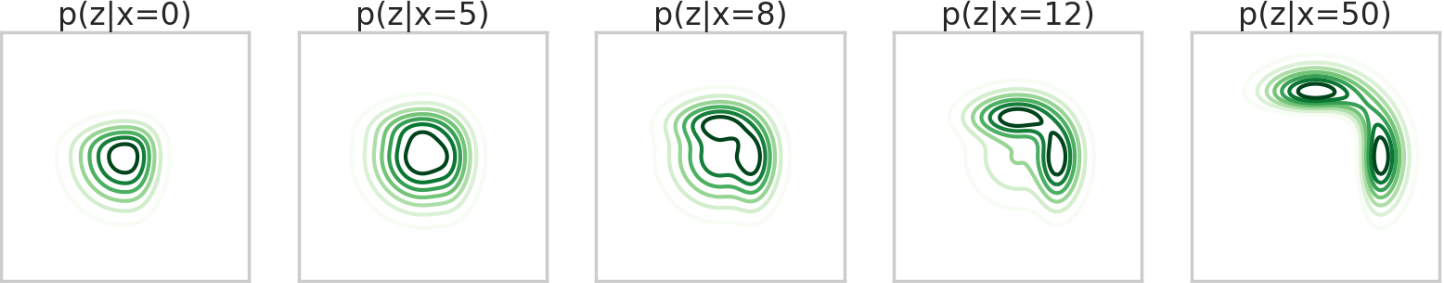
\includegraphics[width=\textwidth]{sprinklertrue.png}
\caption{\small This figure depicts the true (unnormalised) posterior plots for the ``Continuous Sprinkler" experiment. As $x$ increases, the posteriors become increasingly multimodal and unusually shaped. Clearly a flexible model for the posterior distribution is required, as a typical multivariate Gaussian model would fail to capture these features.}
\end{figure}
\section{Program Structure}
Recall from Section 3.9.1 that our generator $\mathcal{G}_\phi(x,\epsilon)$ is a neural network that takes in noise $\epsilon\sim \pi(\epsilon)$ along with data sample $x\sim q^*(x)$ to output a sample from the variational posterior distribution $z\sim q_\phi(z|x)$. In this experiment, the generator has 3 noise inputs $\bm{\epsilon}=(\epsilon_1,\epsilon_2,\epsilon_3)^\top \sim \mathcal{N}(0,I_{3\times 3})$ along with 1 data input $x$, and 2 posterior outputs $z_1, z_2$. The structure of the neural network is as depicted in Figure 5.2 below:
\begin{figure}[h!]
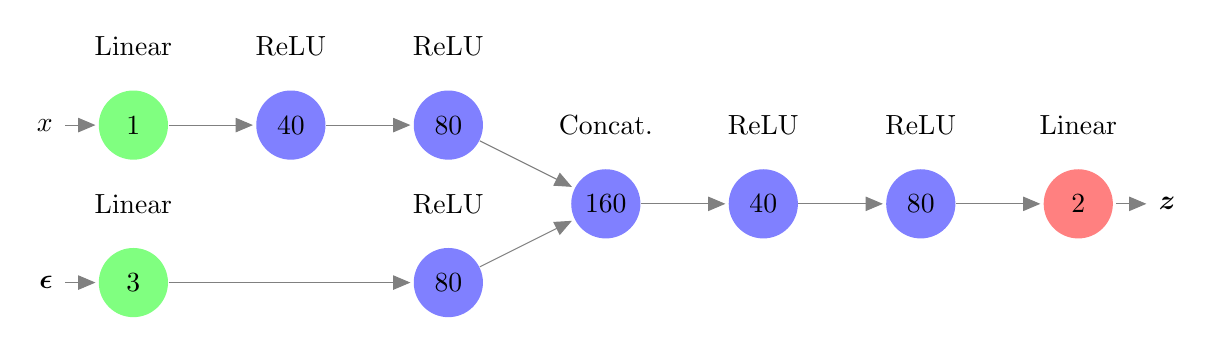
\begin{tikzpicture}[shorten >=1pt,->,draw=black!50, node distance=2.5cm]
    \tikzstyle{every pin edge}=[<-,shorten <=1pt]
    \tikzstyle{neuron}=[circle,fill=black!25,minimum size=25pt,inner sep=0pt]
    \tikzstyle{input neuron}=[neuron, fill=green!50];
    \tikzstyle{output neuron}=[neuron, fill=red!50];
    \tikzstyle{hidden neuron}=[neuron, fill=blue!50];
    \tikzstyle{annot} = [text width=4em, text centered]
    
	%\node[input neuron, pin=left:Bias] (I-0) at (0,0) {$x_0$};
    % Draw the input layer nodes
    %\foreach \name / \y in {1,...,3}
    % This is the same as writing \foreach \name / \y in {1/1,2/2,3/3,4/4}
    \node[input neuron, pin=left:$x$] (I-1) at (0,-1) {$1$};
	\node[input neuron, pin=left:$\bm{\epsilon}$] (I-2) at (0,-3) {$3$};

    \path[yshift=0cm] node[hidden neuron] (H-11) at (2.0cm,-1) {$40$};
	\path[yshift=0cm] node[hidden neuron] (H-12) at (4.0cm,-1) {$80$};
    \path[yshift=0cm] node[hidden neuron] (H-2) at (4.0cm,-3) {$80$};
    \path[yshift=0cm] node[hidden neuron] (H-3) at (6.0cm,-2) {$160$};
    \path[yshift=0cm] node[hidden neuron] (H-31) at (8.0cm,-2) {$40$};
    \path[yshift=0cm] node[hidden neuron] (H-32) at (10.0cm,-2) {$80$};
	\path[yshift=0cm] node[output neuron,pin={[pin edge={->}]right:$\bm{z}$}] (O) at (12.0cm, -2) {$2$};
    \path (I-1) edge (H-11);
    \path (H-11) edge (H-12);
	\path (I-2) edge (H-2);
	\path (H-12) edge (H-3);
	\path (H-2) edge (H-3);
	\path (H-3) edge (H-31);
	\path (H-31) edge (H-32);
	\path (H-32) edge (O);
    % Annotate the layers
    \node[annot,above of=I-1, node distance=1cm] {Linear};
    \node[annot,above of=I-2, node distance=1cm] {Linear};
    \node[annot,above of=H-11, node distance=1cm] {ReLU};
    \node[annot,above of=H-12, node distance=1cm] {ReLU};
    \node[annot,above of=H-2, node distance=1cm] {ReLU};
    \node[annot,above of=H-3, node distance=1cm] {Concat.};
    \node[annot,above of=H-31, node distance=1cm] {ReLU};
    \node[annot,above of=H-32, node distance=1cm] {ReLU};
    \node[annot,above of=O, node distance=1cm] {Linear};
\end{tikzpicture}
\caption{\small This figure illustrates the structure of the generator network $\mathcal{G}(x,\bm{\epsilon})$ used in the ``Continuous Sprinkler" experiment. The number inside the node indicates how many nodes the layer has, and the text above the node describes the activation function. Recall that the input layer does not have an activation function, and Rectified Linear Units (ReLU) are used for most of the hidden layers due to their many advantages. In the Concat. layer, the two input vectors are concatenated and there is no activation function. We do not use an activation function for the output layer as $q_\phi(z|x)\in \R$.}
\end{figure}\\
The structure of the estimator (discriminator $D_\alpha(z,x)$ or ratio estimator $r_\alpha(z,x)$) is similar to that of the the generator, with an additional hidden layer associated with the $z$ input and a different activation function for the output layer, corresponding to the estimator's identity. Note that the only differences between the two estimators are the activation function of the their output layers and the loss functions being minimised. The estimator structure is shown in Figure 5.3 below:
\begin{figure}[h!]

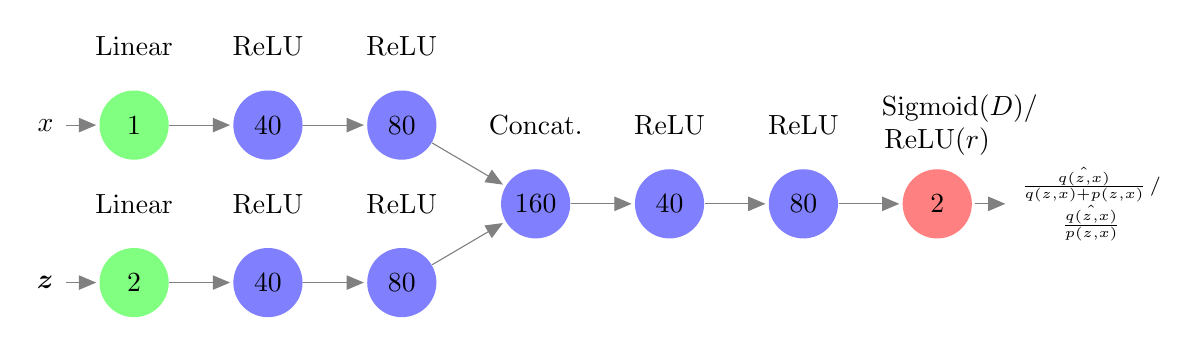
\begin{tikzpicture}[shorten >=1pt,->,draw=black!50, node distance=2.5cm]
    \tikzstyle{every pin edge}=[<-,shorten <=1pt]
    \tikzstyle{neuron}=[circle,fill=black!25,minimum size=25pt,inner sep=0pt]
    \tikzstyle{input neuron}=[neuron, fill=green!50];
    \tikzstyle{output neuron}=[neuron, fill=red!50];
    \tikzstyle{hidden neuron}=[neuron, fill=blue!50];
    \tikzstyle{annot} = [text width=4em, text centered]
    
	%\node[input neuron, pin=left:Bias] (I-0) at (0,0) {$x_0$};
    % Draw the input layer nodes
    %\foreach \name / \y in {1,...,3}
    % This is the same as writing \foreach \name / \y in {1/1,2/2,3/3,4/4}
    \node[input neuron, pin=left:$x$] (I-1) at (0,-1) {$1$};
	\node[input neuron, pin=left:$\bm{z}$] (I-2) at (0,-3) {$2$};

    \path[yshift=0cm] node[hidden neuron] (H-11) at (1.7cm,-1) {$40$};
	\path[yshift=0cm] node[hidden neuron] (H-12) at (3.4cm,-1) {$80$};
	\path[yshift=0cm] node[hidden neuron] (H-21) at (1.7cm,-3) {$40$};
    \path[yshift=0cm] node[hidden neuron] (H-22) at (3.4cm,-3) {$80$};
    \path[yshift=0cm] node[hidden neuron] (H-3) at (5.1cm,-2) {$160$};
    \path[yshift=0cm] node[hidden neuron] (H-31) at (6.8cm,-2) {$40$};
    \path[yshift=0cm] node[hidden neuron] (H-32) at (8.5cm,-2) {$80$};
	\path[yshift=0cm] node[output neuron,pin={[pin edge={->}]right:$\genfrac{}{}{0pt}{}{\hat{\frac{q(z,x)}{q(z,x)+p(z,x)}}\left.\right/}{\hat{\frac{q(z,x)}{p(z,x)}}}$}] (O) at (10.2cm, -2) {$2$};
    \path (I-1) edge (H-11);
    \path (H-11) edge (H-12);
	\path (I-2) edge (H-21);
	\path (H-21) edge (H-22);
	\path (H-12) edge (H-3);
	\path (H-22) edge (H-3);
	\path (H-3) edge (H-31);
	\path (H-31) edge (H-32);
	\path (H-32) edge (O);
    % Annotate the layers
    \node[annot,above of=I-1, node distance=1cm] {Linear};
    \node[annot,above of=I-2, node distance=1cm] {Linear};
    \node[annot,above of=H-11, node distance=1cm] {ReLU};
    \node[annot,above of=H-12, node distance=1cm] {ReLU};
    \node[annot,above of=H-21, node distance=1cm] {ReLU};
    \node[annot,above of=H-22, node distance=1cm] {ReLU};
    \node[annot,above of=H-3, node distance=1cm] {Concat.};
    \node[annot,above of=H-31, node distance=1cm] {ReLU};
    \node[annot,above of=H-32, node distance=1cm] {ReLU};
    \node[annot,above of=O, node distance=1cm] {Sigmoid($D$)/ ReLU($r$)};
\end{tikzpicture}
\caption{\small This figure depicts the structure of the estimator network for the ``Continuous Sprinkler Experiment". The notation is the same as in Figure 5.2. When the estimator takes the parametrisation of a discriminator $D_\alpha(z,x)\simeq \frac{q(z,x)}{q(z,x)+p(z,x)}$, a sigmoid activation function is used for the output layer \citep{gan}. A ReLU output layer is used when the estimator output is the direct density ratio $r_\alpha(z,x)\simeq \frac{q(z,x)}{p(z,x)}$ \citep{relu1, relu2}.}
\end{figure}
\newpage
The network weights are initialized with Xavier initialization, and trained using the Adam optimizer with learning rate $0.0001$ for the prior-contrastive setting and $0.00001$ for joint-contrastive. Preliminary tests show that these are the highest learning rates at which both families of algorithms converge consistently; any higher learning rates lead to the direct ratio estimator in divergence minimisation consistently entering a ``failure" state. This scenario is discussed in section 5.3.

The network is only trained on data values $x=0,5,8,12,50$. In each training iteration, 200 samples are taken for each x-value, corresponding to a batch size of 1000. This large batch size makes training more consistent, as the samples are probabilistic in nature. Due to the similar network structure in both algorithms, they have near-identical runtime, as the majority of the training time is spent in back-propagation \citep{DeepLearning}.

To prevent problems with taking $\log 0$ in the loss functions, we add a small constant $c=10^{-18}$ to the log function's input. The estimator is pre-trained for 5000 iterations to ensure that optimization of the variational network begins with an optimal estimator; an inaccurate ratio estimation leads to incorrect optimization of the posterior network. The variance of the results is also reduced as the initial parametrisation of the estimator will be approximately the same for a fixed generator initialization. Afterwards, the generator is optimized for 10000 iterations when we have an implicit prior, and 40000 iterations in the joint-contrastive formulation. The algorithm alternates between 100 training steps of the estimator and 1 training step of the generator. The processes for class probability estimation and divergence minimisation, based off the algorithms derived in chapter 4, are shown in Algorithms 8 and 9 on the following pages.

We evaluate the techniques by comparing the average KL divergence between the true and variational posteriors at the end of the program's runtime: \[\E_{q^*(x)}KL(q_\phi(\bm{z}|x)\|p(\bm{z}|x)).\] To do so, we estimate the probability density function of the variational posterior output for each of the 5 data points with a Gaussian kernel density estimator $\hat{q}(\bm{z}|x)$. We also use the unnormalised true posterior as derived in equation (5.1.1). The normalisation constant $p(x)$ is the same regardless of the variational posterior $q_\phi(\bm{z}|x)$ that we compare it with, so its omission has no impact on our comparison of the algorithms. This density estimation technique is suitable for our low dimensional problem, and the accuracy is independent of the algorithm used. An explanation of kernel density estimation can be found in Appendix A. Due to the stochastic nature of the optimisation, it is desirable to have a high number of experiment repetitions for reliable results. However, we have limited computational time available, so each algorithm was run 30 times. At the end of each posterior optimisation step, the estimator loss and NELBO estimation was stored. Every 100 iterations, kernel density estimation was used to estimate the true average KL divergence.
\begin{algorithm}
\SetKw{update}{update}
\caption{Sprinkler Prior-Contrastive Algorithm}
\KwData{Dataset $q^*(x)=\{0,5,8,12,20\}$,\\ (Implicit) Prior $p(z)\sim \mathcal{N}(0,2I_{2\times 2})$,\\ Likelihood $p(x|z)\sim EXP(3+\max(0,z_1)^3+\max(0,z_2)^3)$,\\ Noise distribution $\pi(\epsilon)\sim \mathcal{N}(0,I_{3\times 3})$}
\KwResult{Optimized posterior generator $\mathcal{G}_\phi(\epsilon;x)$}
\BlankLine
\For{$j=1$ \KwTo $5000$}{
	Sample $\{\epsilon^{(i,j)}\}^{1000}_{i=1}\sim \pi(\epsilon)$\;
		Sample $\{0,5,8,12,50\}^{200}_{i=1}=\{x^{(i,j)}\}^{1000}_{i=1}\sim q^*(x)$\;
		Sample $\{z^{(i,j)}_p\}^{1000}_{i=1}\sim p(z)$\;
		\ForEach{$\epsilon^{(i,j)},x^{(i,j)}$}{
			Sample $z^{(i,j)}_q=\mathcal{G}(\epsilon^{(i,j)};x^{(i,j}_q)$\;
		}
		\update{Estimator weights $\alpha$}
}
\For{$j=1$ \KwTo $10000$}{
	\For{$k=1$ \KwTo $100$}{	
		Sample $\{\epsilon^{(i,k)}\}^{1000}_{i=1}\sim \pi(\epsilon)$\;
		Sample $\{0,5,8,12,50\}^{200}_{i=1}=\{x^{(i,k)}\}^{1000}_{i=1}\sim q^*(x)$\;
		Sample $\{z^{(i,k)}_p\}^{1000}_{i=1}\sim p(z)$\;
		\ForEach{$\epsilon^{(i,k)},x^{(i,k)}$}{
			Sample $z^{(i,k)}_q=\mathcal{G}(\epsilon^{(i,k)};x^{(i,k)}_q)$\;
		}
		\update{Estimator weights $\alpha$}
	}
	Sample $\{\epsilon^{(i)}\}^{1000}_{i=1}\sim \pi(\epsilon)$\;
	Sample $\{0,5,8,12,50\}^{200}_{i=1}=\{x^{(i)}\}^{1000}_{i=1}\sim q^*(x)$\;
	\update{Variational posterior weights $\phi$}
}
\end{algorithm}
%\begin{algorithm}
%\SetKw{update}{update}
%\caption{Sprinkler Prior-Contrastive Class Probability Estimation}
%\KwData{Dataset $q^*(x)=\{0,5,8,12,20\}$,\\ (Implicit) Prior $p(z)\sim \mathcal{N}(0,2I_{2\times 2})$,\\ Likelihood $p(x|z)\sim EXP(3+\max(0,z_1)^3+\max(0,z_2)^3)$,\\ Noise distribution $\pi(\epsilon)\sim \mathcal{N}(0,I_{3\times 3})$}
%\KwResult{Optimized posterior generator $\mathcal{G}_\phi(\epsilon;x)$}
%\BlankLine
%\For{$j=1$ \KwTo $5000$}{
%	Sample $\{\epsilon^{(i,j)}\}^{1000}_{i=1}\sim \pi(\epsilon)$\;
%		Sample $\{0,5,8,12,50\}^{200}_{i=1}=\{x^{(i,j)}\}^{1000}_{i=1}\sim q^*(x)$\;
%		Sample $\{z^{(i,j)}_p\}^{1000}_{i=1}\sim p(z)$\;
%		\ForEach{$\epsilon^{(i,j)},x^{(i,j)}$}{
%			Sample $z^{(i,j)}_q=\mathcal{G}(\epsilon^{(i,j)};x^{(i,j}_q)$\;
%		}
%		\update{$\alpha$ by optimization step on}{
%			$\min_\alpha -\frac{1}{1000}\sum_{i=1}^{1000}\{\log [D_\alpha(\mathcal{G}_\phi(\epsilon^{(i,j)};x^{(i,j)}), x^{(i,j)})]+\log [1-D_\alpha(z_p^{(i,j)},x^{(i,j)})]\}$\;
%		}
%}
%\For{$j=1$ \KwTo $10000$}{
%	\For{$k=1$ \KwTo $100$}{	
%		Sample $\{\epsilon^{(i,k)}\}^{1000}_{i=1}\sim \pi(\epsilon)$\;
%		Sample $\{0,5,8,12,50\}^{200}_{i=1}=\{x^{(i,k)}\}^{1000}_{i=1}\sim q^*(x)$\;
%		Sample $\{z^{(i,k)}_p\}^{1000}_{i=1}\sim p(z)$\;
%		\ForEach{$\epsilon^{(i,k)},x^{(i,k)}$}{
%			Sample $z^{(i,k)}_q=\mathcal{G}(\epsilon^{(i,k)};x^{(i,k)}_q)$\;
%		}
%		\update{$\alpha$ by optimization step on}{
%			$\min_\alpha -\frac{1}{1000}\sum_{i=1}^{1000}\{\log [D_\alpha(\mathcal{G}_\phi(\epsilon^{(i,k)};x^{(i,k)}), x^{(i,k)})]+\log [1-D_\alpha(z_p^{(i,k)},x^{(i,k)})]\}$\;
%		}
%	}
%	Sample $\{\epsilon^{(i)}\}^{1000}_{i=1}\sim \pi(\epsilon)$\;
%	Sample $\{0,5,8,12,50\}^{200}_{i=1}=\{x^{(i)}\}^{1000}_{i=1}\sim q^*(x)$\;
%	\update{$\phi$ by optimization step on}{
%		$\min_\phi \frac{1}{1000}\sum^{1000}_{i=1}\{-\log p(x|\mathcal{G}_\phi(\epsilon^{(i)};x^{(i)}))+\log\frac{D_\alpha(\mathcal{G}_\phi(\epsilon^{(i)};x^{(i)}),x^{(i)})}{1-D_\alpha(\mathcal{G}_\phi(\epsilon^{(i)};x^{(i)}),x^{(i)})}\}$\;
%	}
%}
%\end{algorithm}
%\begin{algorithm}
%\SetKw{update}{update}
%\caption{Sprinkler Prior-Contrastive KL Divergence Minimisation}
%\KwData{Dataset $q^*(x)=\{0,5,8,12,20\}$,\\ (Implicit) Prior $p(z)\sim \mathcal{N}(0,2I_{2\times 2})$,\\ Likelihood $p(x|z)\sim EXP(3+\max(0,z_1)^3+\max(0,z_2)^3)$,\\ Noise distribution $\pi(\epsilon)\sim \mathcal{N}(0,I_{3\times 3})$}
%\KwResult{Optimized posterior generator $\mathcal{G}_\phi(\epsilon;x)$}
%\BlankLine
%\For{$j=1$ \KwTo $5000$}{
%	Sample $\{\epsilon^{(i,j)}\}^{1000}_{i=1}\sim \pi(\epsilon)$\;
%		Sample $\{0,5,8,12,50\}^{200}_{i=1}=\{x^{(i,j)}\}^{1000}_{i=1}\sim q^*(x)$\;
%		Sample $\{z^{(i,j)}_p\}^{1000}_{i=1}\sim p(z)$\;
%		\ForEach{$\epsilon^{(i,j)},x^{(i,j)}$}{
%			Sample $z^{(i,j)}_q=\mathcal{G}(\epsilon^{(i,j)};x^{(i,j})$\;
%		}
%		\update{$\alpha$ by optimization step on}{
%			$\min_\alpha -\frac{1}{1000}\sum_{i=1}^{1000}\{\log [r_\alpha(\mathcal{G}_\phi(\epsilon^{(i,j)};x^{(i,j)}), x^{(i,j)})]+r_\alpha(z_p^{(i,j)},x^{(i,j)})\}$\;
%		}
%}
%\For{$j=1$ \KwTo $10000$}{
%	\For{$k=1$ \KwTo $100$}{	
%		Sample $\{\epsilon^{(i,k)}\}^{1000}_{i=1}\sim \pi(\epsilon)$\;
%		Sample $\{0,5,8,12,50\}^{200}_{i=1}=\{x^{(i,k)}\}^{1000}_{i=1}\sim q^*(x)$\;
%		Sample $\{z^{(i,k)}_p\}^{1000}_{i=1}\sim p(z)$\;
%		\ForEach{$\epsilon^{(i,k)},x^{(i,k)}$}{
%			Sample $z^{(i,k)}_q=\mathcal{G}(\epsilon^{(i,k)};x^{(i,k)}_q)$\;
%		}
%		\update{$\alpha$ by optimization step on}{
%			$\min_\alpha -\frac{1}{1000}\sum_{i=1}^{1000}\{\log [r_\alpha(\mathcal{G}_\phi(\epsilon^{(i,k)};x^{(i,k)}), x^{(i,k)})]+r_\alpha(z_p^{(i,k)},x^{(i,k)})\}$\;
%		}
%	}
%	Sample $\{\epsilon^{(i)}\}^{1000}_{i=1}\sim \pi(\epsilon)$\;
%	Sample $\{0,5,8,12,50\}^{200}_{i=1}=\{x^{(i)}\}^{1000}_{i=1}\sim q^*(x)$\;
%	\update{$\phi$ by optimization step on}{
%		$\min_\phi \frac{1}{1000}\sum^{1000}_{i=1}\{-\log p(x|\mathcal{G}_\phi(\epsilon^{(i)};x^{(i)}))+\log r_\alpha(\mathcal{G}_\phi(\epsilon^{(i)};x^{(i)}),x^{(i)})\}$\;
%	}
%}
%\end{algorithm}
\begin{algorithm}
\SetKw{update}{update}
\caption{Sprinkler Joint-Contrastive Algorithm}
\KwData{Dataset $q^*(x)=\{0,5,8,12,20\}$,\\ (Implicit) Prior $p(z)\sim \mathcal{N}(0,2I_{2\times 2})$,\\ (Implicit) Likelihood $p(x|z)\sim EXP(3+\max(0,z_1)^3+\max(0,z_2)^3)$,\\ Noise distribution $\pi(\epsilon)\sim \mathcal{N}(0,I_{3\times 3})$}
\KwResult{Optimized posterior generator $\mathcal{G}_\phi(\epsilon;x)$}
\BlankLine
\For{$j=1$ \KwTo $5000$}{
	Sample $\{\epsilon^{(i,j)}\}^{1000}_{i=1}\sim \pi(\epsilon)$\;
		Sample $\{0,5,8,12,50\}^{200}_{i=1}=\{x^{(i,j)}_q\}^{1000}_{i=1}\sim q^*(x)$\;
		Sample $\{z^{(i,j)}_p\}^{1000}_{i=1}\sim p(z)$\;
		\ForEach{$\epsilon^{(i,j)},x^{(i,j)}$}{
			Sample $z^{(i,j)}_q=\mathcal{G}(\epsilon^{(i,j)};x^{(i,j}_q)$\;
		}
		\ForEach{$z^{(i,j)}_p$}{
			Sample $x^{(i,j)}_p\sim p(x|z)$\;
		}
		\update{Estimator weights $\alpha$}
}
\For{$j=1$ \KwTo $40000$}{
	\For{$k=1$ \KwTo $100$}{	
		Sample $\{\epsilon^{(i,k)}\}^{1000}_{i=1}\sim \pi(\epsilon)$\;
		Sample $\{0,5,8,12,50\}^{200}_{i=1}=\{x^{(i,k)}_q\}^{1000}_{i=1}\sim q^*(x)$\;
		Sample $\{z^{(i,k)}_p\}^{1000}_{i=1}\sim p(z)$\;
		\ForEach{$\epsilon^{(i,k)},x^{(i,k)}$}{
			Sample $z^{(i,k)}_q=\mathcal{G}(\epsilon^{(i,k)};x^{(i,k)}_q)$\;
		}
		\ForEach{$z^{(i,k)}_p$}{
			Sample $x^{(i,k)}_p\sim p(x|z)$\;
		}
		\update{Estimator weights $\alpha$}
	}
	Sample $\{\epsilon^{(i)}\}^{1000}_{i=1}\sim \pi(\epsilon)$\;
	Sample $\{0,5,8,12,50\}^{200}_{i=1}=\{x^{(i)}_q\}^{1000}_{i=1}\sim q^*(x)$\;
	\update{Variational posterior weights $\phi$}
}
\end{algorithm}
%\begin{algorithm}
%\SetKw{update}{update}
%\caption{Sprinkler Joint-Contrastive Class Probability Estimation}
%\KwData{Dataset $q^*(x)=\{0,5,8,12,20\}$,\\ (Implicit) Prior $p(z)\sim \mathcal{N}(0,2I_{2\times 2})$,\\ (Implicit) Likelihood $p(x|z)\sim EXP(3+\max(0,z_1)^3+\max(0,z_2)^3)$,\\ Noise distribution $\pi(\epsilon)\sim \mathcal{N}(0,I_{3\times 3})$}
%\KwResult{Optimized posterior generator $\mathcal{G}_\phi(\epsilon;x)$}
%\BlankLine
%\For{$j=1$ \KwTo $5000$}{
%	Sample $\{\epsilon^{(i,j)}\}^{1000}_{i=1}\sim \pi(\epsilon)$\;
%		Sample $\{0,5,8,12,50\}^{200}_{i=1}=\{x^{(i,j)}_q\}^{1000}_{i=1}\sim q^*(x)$\;
%		Sample $\{z^{(i,j)}_p\}^{1000}_{i=1}\sim p(z)$\;
%		\ForEach{$\epsilon^{(i,j)},x^{(i,j)}$}{
%			Sample $z^{(i,j)}_q=\mathcal{G}(\epsilon^{(i,j)};x^{(i,j}_q)$\;
%		}
%		\ForEach{$z^{(i,j)}_p$}{
%			Sample $x^{(i,j)}_p\sim p(x|z)$\;
%		}
%		\update{$\alpha$ by optimization step on}{
%			$\min_\alpha -\frac{1}{1000}\sum_{i=1}^{1000}\{\log [D_\alpha(\mathcal{G}_\phi(\epsilon^{(i,j)};x_q^{(i,j)}), x_q^{(i,j)})]+\log [1-D_\alpha(z_p^{(i,j)},x_p^{(i,j)})]\}$\;
%		}
%}
%\For{$j=1$ \KwTo $40000$}{
%	\For{$k=1$ \KwTo $100$}{	
%		Sample $\{\epsilon^{(i,k)}\}^{1000}_{i=1}\sim \pi(\epsilon)$\;
%		Sample $\{0,5,8,12,50\}^{200}_{i=1}=\{x^{(i,k)}_q\}^{1000}_{i=1}\sim q^*(x)$\;
%		Sample $\{z^{(i,k)}_p\}^{1000}_{i=1}\sim p(z)$\;
%		\ForEach{$\epsilon^{(i,k)},x^{(i,k)}$}{
%			Sample $z^{(i,k)}_q=\mathcal{G}(\epsilon^{(i,k)};x^{(i,k)}_q)$\;
%		}
%		\ForEach{$z^{(i,k)}_p$}{
%			Sample $x^{(i,k)}_p\sim p(x|z)$\;
%		}
%		\update{$\alpha$ by optimization step on}{
%			$\min_\alpha -\frac{1}{1000}\sum_{i=1}^{1000}\{\log [D_\alpha(\mathcal{G}_\phi(\epsilon^{(i,k)};x_q^{(i,k)}), x_q^{(i,k)})]+\log [1-D_\alpha(z_p^{(i,k)},x_p^{(i,k)})]\}$\;
%		}
%	}
%	Sample $\{\epsilon^{(i)}\}^{1000}_{i=1}\sim \pi(\epsilon)$\;
%	Sample $\{0,5,8,12,50\}^{200}_{i=1}=\{x^{(i)}_q\}^{1000}_{i=1}\sim q^*(x)$\;
%	\update{$\phi$ by optimization step on}{
%		$\min_\phi \frac{1}{1000}\sum^{1000}_{i=1}\log\frac{D_\alpha(\mathcal{G}_\phi(\epsilon^{(i)};x_q^{(i)}),x_q^{(i)})}{1-D_\alpha(\mathcal{G}_\phi(\epsilon^{(i)};x_q^{(i)}),x_q^{(i)})}$\;
%	}
%}
%\end{algorithm}
%\begin{algorithm}
%\SetKw{update}{update}
%\caption{Sprinkler Joint-Contrastive KL Divergence Minimisation}
%\KwData{Dataset $q^*(x)=\{0,5,8,12,20\}$,\\ (Implicit) Prior $p(z)\sim \mathcal{N}(0,2I_{2\times 2})$,\\ (Implicit) Likelihood $p(x|z)\sim EXP(3+\max(0,z_1)^3+\max(0,z_2)^3)$,\\ Noise distribution $\pi(\epsilon)\sim \mathcal{N}(0,I_{3\times 3})$}
%\KwResult{Optimized posterior generator $\mathcal{G}_\phi(\epsilon;x)$}
%\BlankLine
%\For{$j=1$ \KwTo $5000$}{
%	Sample $\{\epsilon^{(i,j)}\}^{1000}_{i=1}\sim \pi(\epsilon)$\;
%		Sample $\{0,5,8,12,50\}^{200}_{i=1}=\{x^{(i,j)}_q\}^{1000}_{i=1}\sim q^*(x)$\;
%		Sample $\{z^{(i,j)}_p\}^{1000}_{i=1}\sim p(z)$\;
%		\ForEach{$\epsilon^{(i,j)},x^{(i,j)}$}{
%			Sample $z^{(i,j)}_q=\mathcal{G}(\epsilon^{(i,j)};x^{(i,j}_q)$\;
%		}
%		\ForEach{$z^{(i,j)}_p$}{
%			Sample $x^{(i,j)}_p\sim p(x|z)$\;
%		}
%		\update{$\alpha$ by optimization step on}{
%			$\min_\alpha -\frac{1}{1000}\sum_{i=1}^{1000}\{\log [r_\alpha(\mathcal{G}_\phi(\epsilon^{(i,j)};x_q^{(i,j)}), x_q^{(i,j)})]+r_\alpha(z_p^{(i,j)},x_p^{(i,j)})\}$\;
%		}
%}
%\For{$j=1$ \KwTo $40001$}{
%	\For{$k=1$ \KwTo $100$}{	
%		Sample $\{\epsilon^{(i,k)}\}^{1000}_{i=1}\sim \pi(\epsilon)$\;
%		Sample $\{0,5,8,12,50\}^{200}_{i=1}=\{x^{(i,k)}_q\}^{1000}_{i=1}\sim q^*(x)$\;
%		Sample $\{z^{(i,k)}_p\}^{1000}_{i=1}\sim p(z)$\;
%		\ForEach{$\epsilon^{(i,k)},x^{(i,k)}$}{
%			Sample $z^{(i,k)}_q=\mathcal{G}(\epsilon^{(i,k)};x^{(i,k)}_q)$\;
%		}
%		\ForEach{$z^{(i,k)}_p$}{
%			Sample $x^{(i,k)}_p\sim p(x|z)$\;
%		}
%		\update{$\alpha$ by optimization step on}{
%			$\min_\alpha -\frac{1}{1000}\sum_{i=1}^{1000}\{\log [r_\alpha(\mathcal{G}_\phi(\epsilon^{(i,k)};x_q^{(i,k)}), x_q^{(i,k)})]+r_\alpha(z_p^{(i,k)},x_p^{(i,k)})\}$\;
%		}
%	}
%	Sample $\{\epsilon^{(i)}\}^{1000}_{i=1}\sim \pi(\epsilon)$\;
%	Sample $\{0,5,8,12,50\}^{200}_{i=1}=\{x^{(i)}_q\}^{1000}_{i=1}\sim q^*(x)$\;
%	\update{$\phi$ by optimization step on}{
%		$\min_\phi \frac{1}{1000}\sum^{1000}_{i=1}\log r_\alpha(\mathcal{G}_\phi(\epsilon^{(i)};x_q^{(i)}),x_q^{(i)})$\;
%	}
%}
%\end{algorithm}
\newpage
\section{Results}
The mean and standard deviation of the estimated average KL divergence %$\E_{q^*(x)}KL(\hat{q}(z|x)\|p(z|x))$
at the end of the program runtime is tabulated in Table 5.1 below. To visually compare the posterior outputs, Gaussian kernel density estimation was used to plot 1000 variational posterior samples for each data point. This is depicted in Figure 5.4 below. The arrays storing the average KL divergences, estimator losses and NELBOs over the iterations were averaged over the 30 repetitions. Plots of these arrays are shown in Figures 5.5-5.7.
\begin{table}[h!]
\begin{tabular}{|c|c|c|}
\hline
Algorithm & Mean KL Divergence & Standard Deviation\\
\hline
PC Divergence Minimisation & 1.3807 & 0.0391\\
\hline
PC Class Probability Estimation & 1.3267 & 0.0041\\
\hline
JC Divergence Minimisation & 1.6954 & 0.4337\\
\hline
JC Class Probability Estimation & 1.3688 & 0.0415\\
\hline
\end{tabular}
\caption{}
\end{table}
\begin{figure}[h!]
\begin{subfigure}{\textwidth}
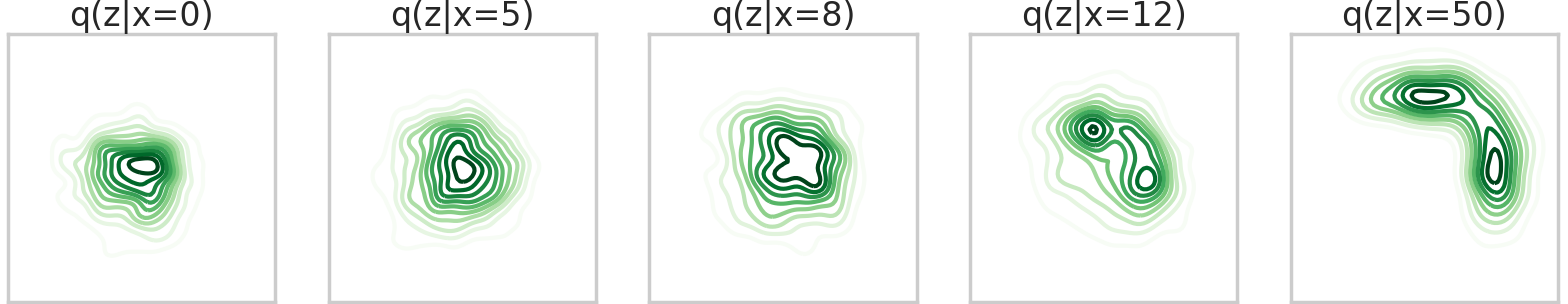
\includegraphics[width=\textwidth]{13288.png}
\caption{Average KL Divergence of 1.3288}
\end{subfigure}
\begin{subfigure}{\textwidth}
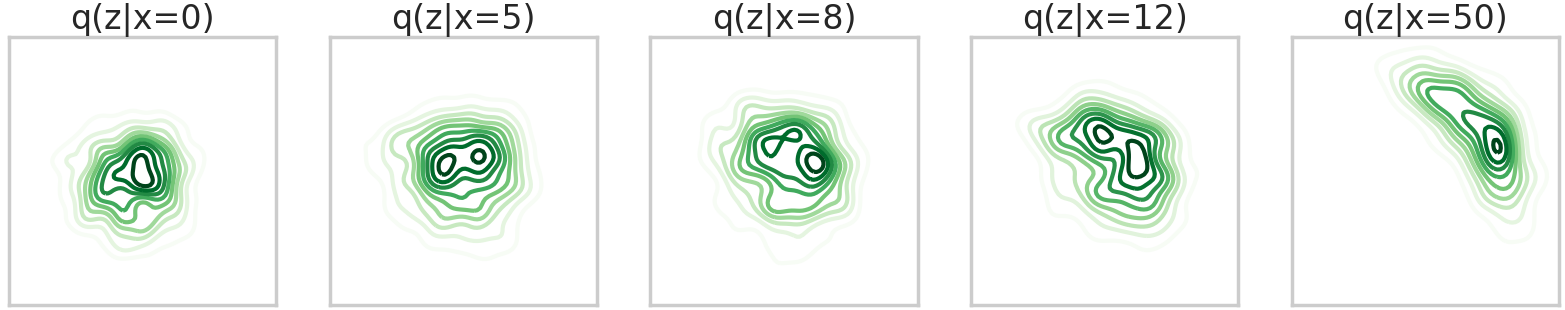
\includegraphics[width=\textwidth]{13963.png}
\caption{Average KL Divergence of 1.3963}
\end{subfigure}
\begin{subfigure}{\textwidth}
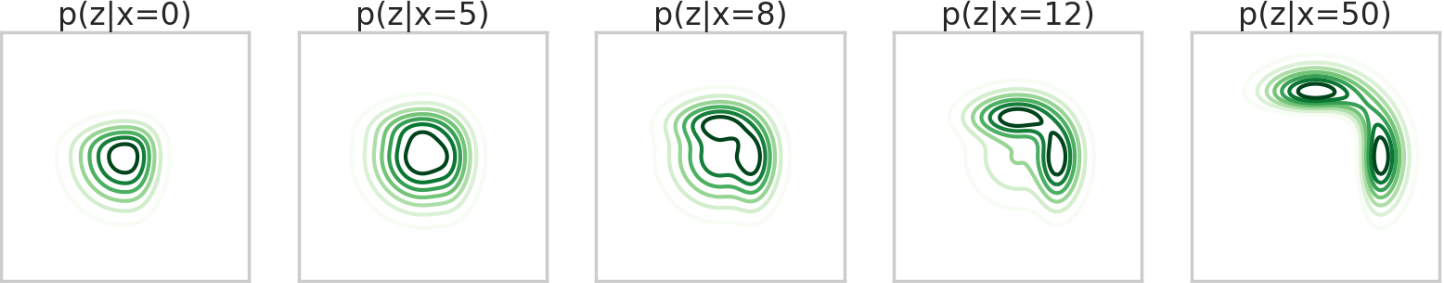
\includegraphics[width=\textwidth]{sprinklertrue}
\caption{True Posterior Plot}
\end{subfigure}
\caption{\small Initial tests show that the variational posterior reaches optimality at an average KL divergence of about 1.325: as seen in sub-figure (a), this corresponds to outputs similar to the true posterior in sub-figure (c). The posterior output in sub-figure (b) with a larger average KL divergence of 1.3963 is less flexible and only uni-modal for $x=50$.}
\end{figure}
\newpage
\begin{figure}[t!]
\begin{subfigure}{0.49\textwidth}
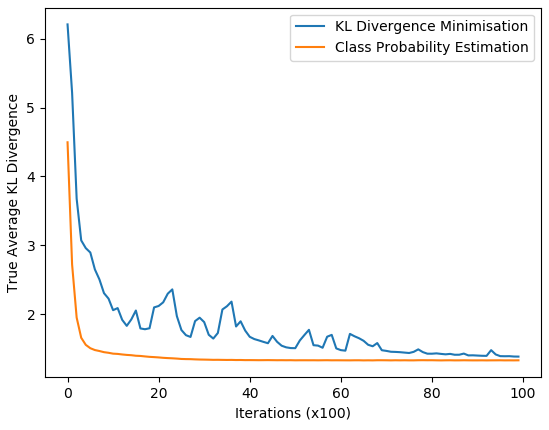
\includegraphics[width=\linewidth]{truklmins/PCKLvsPCADV.png}
\caption{Prior-Contrastive}
\end{subfigure}
\begin{subfigure}{0.49\textwidth}
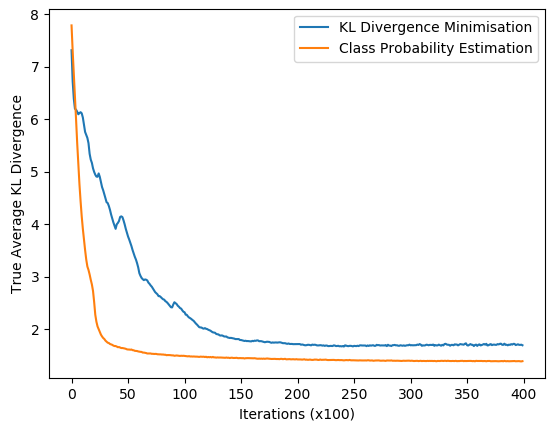
\includegraphics[width=\linewidth]{truklmins/JCKLvsJCADV.png}
\caption{Joint-Contrastive}
\end{subfigure}
\caption{Average KL Divergences (KDE Estimate)}
\end{figure}
\begin{figure}[h!]
\begin{subfigure}{0.49\textwidth}
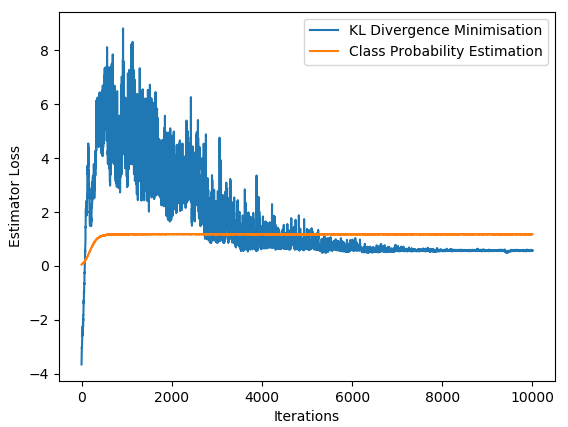
\includegraphics[width=\linewidth]{estimator_losses/PCKLvsPCADV.png}
\caption{Prior-Contrastive}
\end{subfigure}
\begin{subfigure}{0.49\textwidth}
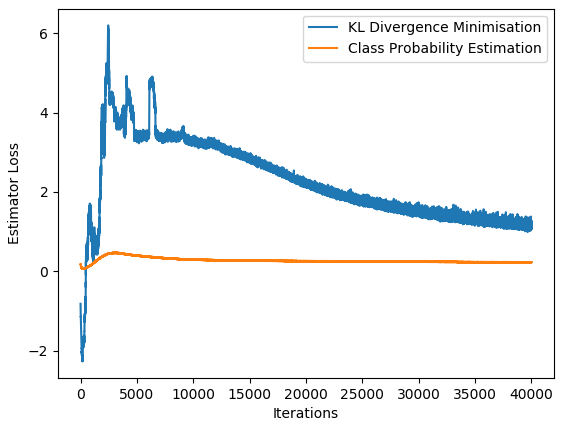
\includegraphics[width=\linewidth]{estimator_losses/JCKLvsJCADV.png}
\caption{Joint-Contrastive}
\end{subfigure}
\caption{Estimator Losses}
\end{figure}
%\begin{figure}[h]
%\begin{subfigure}{0.5\textwidth}
%\includegraphics[width=\linewidth]{•}
%\caption{Prior-Contrastive}
%\end{subfigure}
%\begin{subfigure}{0.5\textwidth}
%\includegraphics[width=\linewidth]{•}
%\caption{Joint-Contrastive}
%\end{subfigure}
%\caption{}
%\end{figure}
\begin{figure}[h!]
\begin{subfigure}{0.49\textwidth}
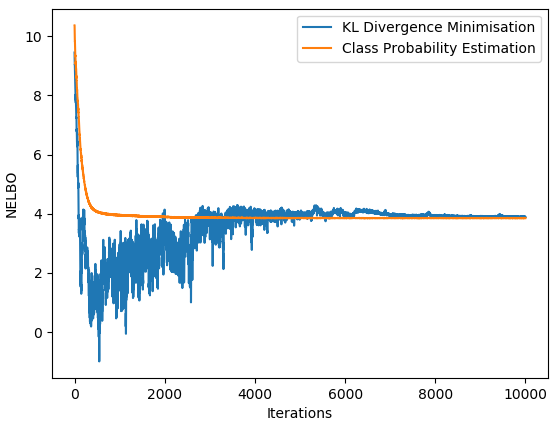
\includegraphics[width=\linewidth]{nelbos/PCKLvsPCADV.png}
\caption{Prior-Contrastive}
\end{subfigure}
\begin{subfigure}{0.49\textwidth}
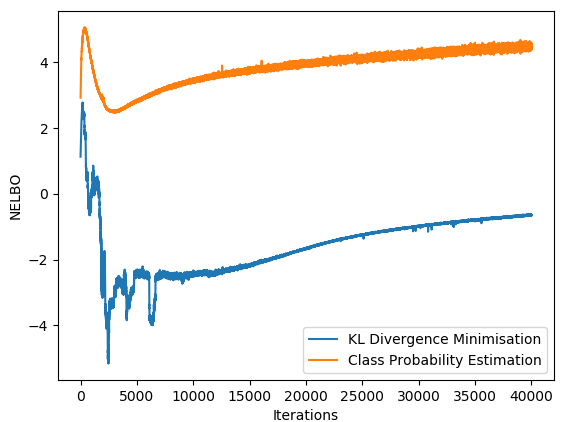
\includegraphics[width=\linewidth]{nelbos/JCKLvsJCADV.png}
\caption{Joint-Contrastive}
\end{subfigure}
\caption{NELBOs}
\end{figure}
\newpage
As one would expect, the prior-contrastive algorithms converged much faster their joint-contrastive equivalent, as expected since knowledge of the likelihood improves posterior optimization. It is unclear in the joint-contrastive case why the NELBO appears to increase throughout the majority of the iterations. This is inconsistent with the reduction of the KDE estimated KL divergence over the same period, but it justifies our use of a metric independent of the estimator loss or estimated NELBO.

Overall, for both families of algorithms, we found that class probability estimation performed consistently better than KL divergence minimisation. The inconsistency of KL minimisation can be seen in the wild fluctuations early in the estimator loss and NELBO graphs, implying that the NELBO is being estimated inaccurately. This corresponds to the instances in the true KL Divergence graphs where the posterior output worsens over certain periods.

Furthermore, in approximately half of the simulations, the ratio loss of the KL divergence minimisation algorithm would start at a relatively high number (42.3 as opposed to 3.5), and it would be stuck there for the entire runtime of the program; the thousands of iterations spent minimizing the ratio loss did not decrease it. The algorithm was programmed to automatically restart every time this happened.
\newpage
\chapter{Activation Function Experiment}
In this chapter, we fix the `failures' of KL minimisation by suggesting an exponential activation function to replace the ReLU output layer. The two methods are compared in both prior-contrastive and joint-contrastive contexts.
\section{Theory}
The `failures' of the KL minimisation approach involve the estimator loss initialising at $41.4465$ or reaching that value during its runtime, and remaining constant throughout the program runtime. Analysis of the estimator during this occurrence revealed that it was outputting an estimated ratio of $0$. Now recall our estimator loss of
\[-\E_q[\log r_\alpha(z,x)]+\E_p[r_\alpha(z,x)]\]
and the constant term $c=10^{-18}$ that we add to the log input. When $r_\alpha(z,x)=0$, the estimator loss is $-\log [10^{-18}]=41.4465$, which verifies that this is the cause of the `failures'. It can be deduced that the network weights are transforming the estimator input into a negative number, which is mapped to $0$ by the ReLU output layer. Since the gradient of the ReLU function is $0$ for negative inputs, back-propagation will record that the partial derivative of the loss function with respect to the weights is $0$, and therefore gradient descent will fail to update the weights. This is known as the `dying ReLU' problem \citep{sparse}, and in other contexts, it can be fixed using a `leaky ReLU', which has a small slope for negative inputs\citep{leaky}:
\[g(x)=\begin{cases}x & x\geq 0\\ \alpha x & x<0
\end{cases}\]
where $\alpha$ is a small number in $(0,1)$ such as 0.01. However, this allows a negative output, which causes problems with the log function in our estimator loss.

Even when the `dying ReLU' problem does not occur, the estimator loss is still unstable for the majority of the program runtime, leading to an inaccurate NELBO estimation and therefore slower convergence. This is likely caused by the linearity of the ReLU output layer causing an imbalance between density ratios in $(0,1)$ and $(1,\infty)$. Recall that the neural network output ranges in $\R$ before being mapped by the output layer's activation function. The density ratio $\frac{q(u)}{p(u)}$ ranges in $(0,1)$ when $q(u)<p(u)$, and it takes values in $(1,\infty)$ when $q(u)>p(u)$, so to balance the two cases, it is ideal if they are each mapped to by complementary half-spaces, e.g. $\R^-$ maps to $(0,1)$ and $\R^+$ maps to $(1,\infty)$. When the ReLU function is used, there is an infinitely larger space used to represent ratios where $q(u)>p(u)$, and the displacement in network weights required to reach optimality is this case is much greater. For example, if the current estimated ratio is $r(u)=2$ (implying $q(u)=2p(u)$) but we actually have $q(u)=10p(u)$, then the weights would have to change such that the output increases by $8$. On the other hand, if the estimated ratio is $r(u)=\frac12$ (implying $2q(u)=p(u)$), but the true ratio is such that $10q(u)=p(u)$, then the weights only have to displace the output by $\frac25$. The gradient-based optimisation would therefore require small training rates for cases where $r(u)\in (0,1)$ and large training rates when $r(u)\in(1,\infty)$, but this scenario is not accounted for in optimisation algorithms using an adaptive training rate. This leads to the unstable estimator losses seen in Figure 5.6.

The sigmoid output of the class probability estimation approach does not experience this problem. Since $D^*(u)=\frac{q(u)}{q(u)+p(u)}$, we have $D(u)\in(0,\frac12)$ when $q(u)<p(u)$ and $D(u)\in(\frac12,1)$ when $q(u)>p(u)$. The sigmoid activation function $g(x)=\frac{1}{1+e^{-x}}$ maps $\R^-$ to $(0,\frac12)$ and $\R^+$ to $(\frac12,1)$, and therefore the two cases have half-space representations.

Following ``f-GAN: Training Generative Neural Samplers using Variational Divergence Minimization" by \citet{nowozin}, we propose an exponential output activation function $g(x)=e^x$ for the divergence minimisation approach. This activation function maps $\R^-$ to $(0,1)$ and $\R^+$ to $(1,\infty)$, resulting in an even representation for the two cases. Following the same example as before, changing from an estimated ratio of $2$ to $10$ equates to a neural network output displacement of $|\log 10-\log 2|=\log 5$, which is the network change as changing from $\frac12$ to $\frac{1}{10}$: $|\log \frac12-\log\frac{1}{10}|=\log 5$. The first contribution of this thesis will be to compare the ReLU and exponential activation functions for the estimator network used in divergence minimisation density ratio estimation, and to show experimentally that the exponential activation function is more stable and leads to faster posterior convergence.
\section{Experiment Outline}
In this experiment, we compare the activation functions in both prior-contrastive and joint-contrastive contexts, using the exact same experimental set up as described in Chapter 5. The divergence minimisation program is exactly the same, but we now have an additional program that uses an exponential activation function instead of ReLU for the estimator's output layer. To save computational time, we reuse our ReLU results from the previous experiment, only running instances of our new program. Again, we estimate the variational distribution with a Gaussian kernel density estimator to calculate the KL divergence, which we use to evaluate to convergence.
\section{Results}
The mean and standard deviation of the final average KL divergence between the true and variational distributions over 30 experiment repetitions is tabulated in Table 6.1 below. It is evident that the exponential output activation function results in vastly superior posterior convergence, with significantly lower KL divergence mean and standard deviation than the algorithm using a ReLU output. Comparing Table 6.1 with Table 5.1, it can be seen that divergence minimisation with an exponential output produces similar results to class probability estimation. It can be deduced that the perceived inferiority of divergence minimisation is a result of using an inappropriate activation function for the output layer.

We have also taken the average of the arrays storing the average KL divergence, estimator loss and estimated NELBO for each posterior iteration. Plots of these arrays are shown in Figures 6.1-6.3 on the next page.
\begin{table}[h!]
\centering
\begin{tabular}{|c|c|c|}
\hline
Algorithm & Mean KL Divergence & Standard Deviation\\
\hline
PC ReLU Output & 1.3807 & 0.0391\\
\hline
PC Exponential Output & 1.3265 & 0.0045\\
\hline
JC ReLU Output & 1.6954 & 0.4337\\
\hline
JC Exponential Output & 1.3397 & 0.0066\\
\hline
\end{tabular}
\caption{}
\end{table}
\newpage
\begin{figure}[t!]
\begin{subfigure}{0.49\textwidth}
\includegraphics[width=\linewidth]{truklmins/PCKLvsPCKLEXP.png}
\caption{Prior-Contrastive}
\end{subfigure}
\begin{subfigure}{0.49\textwidth}
\includegraphics[width=\linewidth]{truklmins/JCKLvsJCKLEXP.png}
\caption{Joint-Contrastive}
\end{subfigure}
\caption{Average KL Divergences (KDE Estimate)}
\end{figure}
\begin{figure}[h!]
\begin{subfigure}{0.49\textwidth}
\includegraphics[width=\linewidth]{estimator_losses/PCKLvsPCKLEXP.png}
\caption{Prior-Contrastive}
\end{subfigure}
\begin{subfigure}{0.49\textwidth}
\includegraphics[width=\linewidth]{estimator_losses/JCKLvsJCKLEXP.png}
\caption{Joint-Contrastive}
\end{subfigure}
\caption{Estimator Losses}
\end{figure}
\begin{figure}[h!]
\begin{subfigure}{0.49\textwidth}
\includegraphics[width=\linewidth]{nelbos/PCKLvsPCKLEXP.png}
\caption{Prior-Contrastive}
\end{subfigure}
\begin{subfigure}{0.49\textwidth}
\includegraphics[width=\linewidth]{nelbos/JCKLvsJCKLEXP.png}
\caption{Joint-Contrastive}
\end{subfigure}
\caption{NELBOs}
\end{figure}
 The average KL divergence for the exponential output appears to converge much more smoothly, and it is consistently lower than in the ReLU output. For the prior-contrastive case, the estimator loss and estimated NELBO from the program using an exponential activation function is much more stable. However, in the joint-contrastive case, these values show more stability early on, then grow increasingly unstable compared to the ReLU case. It is unclear why this occurs, but it does not appear to have a detrimental impact on posterior convergence, as the average KL divergence is still significantly lower during this period.
\chapter{Algorithm Analysis}
In this chapter, we present the two density ratio estimation techniques in a comparable form, that is, in terms of the relevant f-divergence's lower bound as derived in section 4.2 using Theorem 4.2.1. From this, we generalise the density ratio algorithms to a selection of f-divergence to formulate the lower bound, and a parametrisation of the density ratio estimator. We also suggest a third estimator parametrisation: the direct log density ratio estimator $T_\alpha(u)$. The formal generalisation of density ratio estimation algorithms is the second contribution of this thesis.
\section{Introduction}
First, recall that within each of the prior-contrastive and joint-contrastive formulations, both class probability estimation and divergence minimisation methods use the same loss function to optimise the posterior weights. It is therefore evident that the only differences between the two density ratio estimation techniques are the lower bound of the loss function and the parametrization of the estimator. We demonstrate this by restating the f-divergence lower bounds used to formulate these loss functions, as derived in Section 4.2. For divergence minimisation, the lower bound is achieved using the reverse KL divergence $D_{RKL}(p\|q)=KL[q(u)\|p(u)]$:
\[D_{RKL}(p\|q)\geq \sup_{\alpha}\{\mathbb{E}_{q(u)}[1+\log r_\alpha(u)]-\mathbb{E}_{p(u)}[r_\alpha(u)]\},\]
and class probability estimation follows the GAN divergence $D_{GAN}(p\|q)=2D_{JS}(p\|q)-\log 4$:
\[D_{GAN}(p\|q)\geq \sup_\alpha\{\mathbb{E}_{q(u)}\left[\log \frac{r_\alpha(u)}{r_\alpha(u)+1}\right]-\mathbb{E}_{p(u)}[\log(r_\alpha(u)+1)]\},\]
with equality at $r_\alpha(u)=\frac{q(u)}{p(u)}$.\\
To convert the latter equation to class probability estimation loss function, we have used the estimator transformation $r_\alpha(u)=\frac{D_\alpha(u)}{1-D_\alpha(u)}\iff D_\alpha(u)=\frac{r_\alpha(u)}{r_\alpha(u)+1}$. Since this mapping is bijective and monotonically increasing, the equality of the bound is retained at equivalent points. We can therefore also use this transformation on the lower bound of the reverse KL divergence, deriving its respective loss function as a function of $D_\alpha\simeq \frac{q(u)}{q(u)+p(u)}$ instead of $r_\alpha\simeq \frac{q(u)}{p(u)}$.

We also propose a third estimator parametrisation, the direct log density ratio estimator
\[T_\alpha(u)\simeq \log \frac{q(u)}{p(u)}.\]
This is derived by simply using the transformation $T_\alpha(u)=\log r_\alpha(u)$.
\section{Algorithm Generalisation}
For each f-divergence, we can derive a loss function for each of our three estimator parametrisations.
\subsection{Reverse KL Divergence}
\textbf{Direct Ratio Estimator} $r_\alpha(u)$:
\[\min_\alpha -\mathbb{E}_{q(u)}[\log r_\alpha(u)]+\mathbb{E}_{p(u)}[r_\alpha(u)]\]
\textbf{Class Probability Estimator/Discriminator} $D_\alpha(u)$:
\[\min_\alpha \mathbb{E}_{q(u)}\left[\log \frac{1-D_\alpha(u)}{D_\alpha(u)}\right]+\mathbb{E}_{p(u)}\left[\frac{D_\alpha(u)}{1-D_\alpha(u)}\right]\]
\textbf{Direct Log Ratio Estimator} $T_\alpha(u)$:
\[\min_\alpha -\mathbb{E}_{q(u)}[T_\alpha(u)]+\mathbb{E}_{p(u)}[e^{T_\alpha (u)}]\]
\subsection{GAN Divergence}
\textbf{Direct Ratio Estimator} $r_\alpha(u)$:
\[\min_\alpha \E_{q(u)}\left[\log \frac{r_\alpha(u)+1}{r_\alpha(u)}\right]+\E_{p(u)}[\log (r_\alpha(u)+1)]\]
\textbf{Class Probability Estimator/Discriminator} $D_\alpha(u)$:
\[\min_\alpha -\E_{q(u)}[\log D_\alpha(u)]-\E_{p(u)}[\log (1-D_\alpha(u))]\]
\textbf{Direct Log Ratio Estimator} $T_\alpha(u)$:
\[\min_\alpha \E_{q(u)}\left[\log \frac{e^{T_\alpha(u)}+1}{e^{T_\alpha(u)}}\right]+\E_{p(u)}[\log(e^{T_\alpha(u)}+1)]\]
We have therefore generalised the choice of algorithm for training density ratio estimators to a choice of f-divergence:
\begin{itemize}
\item KL Divergence: $D_{KL}(p\|q)=\mathbb{E}_{q(u)}[1+\log \frac{q(u)}{p(u)}]-\mathbb{E}_{p(u)}\left[\frac{q(u)}{p(u)}\right]$
\item GAN Divergence: $D_{GAN}(p\|q)=\mathbb{E}_{q(u)}\left[\log \frac{q(u)}{q(u)+p(u)}\right]+\mathbb{E}_{p(u)}\left[\log \frac{p(u)}{q(u)+p(u)}\right]$
\end{itemize}
and a choice of estimator parametrization:
\begin{itemize}
\item Direct ratio estimator: $r_\alpha(u)\simeq\frac{q(u)}{p(u)}$
\item ``Class probability" estimator/Discriminator: $D_\alpha(u)\simeq\frac{q(u)}{q(u)+p(u)}$
\item Direct log ratio estimator: $T_\alpha(u)\simeq\log \frac{q(u)}{p(u)}.$
\end{itemize}
The original ``KL divergence minimization approach" simply chooses the KL Divergence and the direct ratio estimator, and ``class probability estimation" uses the CPE Divergence and the ``Class probability" estimator. These are just 2 variations of the 6 available algorithms.
\section{Optimization Algorithms}
The ratio estimator in the posterior loss functions also has to be transformed accordingly. In the following sections we give the specific prior-contrastive and joint-contrastive NELBOs as functions of each estimator parametrisation. For completeness, we also list the two different estimator loss functions for each case, corresponding to the two f-divergences that we have discussed.
\subsection{Prior-Contrastive}
\textbf{Direct Ratio Estimator} $r_\alpha(u)$:
\[\text{Reverse KL: }\min_\alpha -\E_{q^*(x)\pi(\epsilon)}[\log r_\alpha(\mathcal{G}(\epsilon;x),x)]+\E_{p(z)q^*(x)}[r_\alpha(z,x)]\]
\[\text{GAN: }\min_\alpha \E_{q^*(x)\pi(\epsilon)}\left[\log \frac{r_\alpha(\mathcal{G}(\epsilon;x),x)+1}{r_\alpha(\mathcal{G}(\epsilon;x),x)}\right]+\E_{p(z)q^*(x)}[\log(r_\alpha(z,x)+1)]\]
\[\min_\phi-\E_{q^*(x)\pi(\epsilon)}[\log p(x|\mathcal{G}_\phi(\epsilon;x)]+\E_{q^*(x)\pi(\epsilon)}[\log r_\alpha(\mathcal{G}(\epsilon;x),x)]\]
\textbf{Class Probability Estimator/Discriminator} $D_\alpha(u)$:
\[\text{Reverse KL: }\min_\alpha \E_{q^*(x)\pi(\epsilon)}\left[\log \frac{1-D_\alpha(\mathcal{G}(\epsilon;x),x)}{D_\alpha(\mathcal{G}(\epsilon;x),x)}\right]+\E_{p(z)q^*(x)}\left[\frac{D_\alpha(\mathcal{G}(\epsilon;x),x)}{1-D_\alpha(\mathcal{G}(\epsilon;x),x)}\right]\]
\[\text{GAN: }\min_\alpha -\E_{q^*(x)\pi(\epsilon)}[\log D_\alpha(\mathcal{G}(\epsilon;x),x)]-\E_{p(z)q^*(x)}[\log(1-D_\alpha(z,x))]\]
\[\min_\phi-\E_{q^*(x)\pi(\epsilon)}[\log p(x|\mathcal{G}_\phi(\epsilon;x)]+\E_{q^*(x)\pi(\epsilon)}\left[\log \frac{D_\alpha(\mathcal{G}(\epsilon;x),x)}{1-D_\alpha(\mathcal{G}(\epsilon;x),x)}\right]\]
\textbf{Direct Log Ratio Estimator} $T_\alpha(u)$:
\[\text{Reverse KL: }\min_\alpha -\E_{q^*(x)\pi(\epsilon)}[T_\alpha(\mathcal{G}(\epsilon;x),x)]+\E_{p(z)q^*(x)}[\exp(T_\alpha(z,x))]\]
\[\text{GAN: }\min_\alpha \E_{q^*(x)\pi(\epsilon)}\left[\log \frac{e^{T_\alpha(\mathcal{G}(\epsilon;x),x)}+1}{e^{T_\alpha(\mathcal{G}(\epsilon;x),x)}}\right]+\E_{p(z)q^*(x)}[\log(e^{T_\alpha(z,x)}+1)]\]
\[\min_\phi-\E_{q^*(x)\pi(\epsilon)}[\log p(x|\mathcal{G}_\phi(\epsilon;x)]+\E_{q^*(x)\pi(\epsilon)}[T_\alpha(\mathcal{G}(\epsilon;x),x)]\]
\subsection{Joint-Contrastive}
\textbf{Direct Ratio Estimator} $r_\alpha(u)$:
\[\text{Reverse KL: }\min_\alpha -\E_{q^*(x)\pi(\epsilon)}[\log r_\alpha(\mathcal{G}(\epsilon;x),x)]+\E_{p(z)p(x|z)}[r_\alpha(z,x)]\]
\[\text{GAN: }\min_\alpha \E_{q^*(x)\pi(\epsilon)}\left[\log \frac{r_\alpha(\mathcal{G}(\epsilon;x),x)+1}{r_\alpha(\mathcal{G}(\epsilon;x),x)}\right]+\E_{p(z)p(x|z)}[\log(r_\alpha(z,x)+1)]\]
\[\min_\phi \E_{q^*(x)\pi(\epsilon)}\log r_\alpha(\mathcal{G}_\phi(\epsilon;x),x)\]
\textbf{Class Probability Estimator/Discriminator} $D_\alpha(u)$:
\[\text{Reverse KL: }\min_\alpha \E_{q^*(x)\pi(\epsilon)}\left[\log \frac{1-D_\alpha(\mathcal{G}(\epsilon;x),x)}{D_\alpha(\mathcal{G}(\epsilon;x),x)}\right]+\E_{p(z)p(x|z)}\left[\frac{D_\alpha(\mathcal{G}(\epsilon;x),x)}{1-D_\alpha(\mathcal{G}(\epsilon;x),x)}\right]\]
\[\text{GAN: }\min_\alpha -\E_{q^*(x)\pi(\epsilon)}[\log D_\alpha(\mathcal{G}(\epsilon;x),x)]-\E_{p(z)p(x|z)}[\log(1-D_\alpha(z,x))]\]
\[\min_\phi \E_{q^*(x)\pi(\epsilon)}\log \frac{D_\alpha(\mathcal{G}_\phi(\epsilon;x),x)}{1-D_\alpha(\mathcal{G}_\phi(\epsilon;x),x)}\]
\textbf{Direct Log Ratio Estimator} $T_\alpha(u)$:
\[\text{Reverse KL: }\min_\alpha -\E_{q^*(x)\pi(\epsilon)}[T_\alpha(\mathcal{G}(\epsilon;x),x)]+\E_{p(z)p(x|z)}[\exp(T_\alpha(z,x))]\]
\[\text{GAN: }\min_\alpha \E_{q^*(x)\pi(\epsilon)}\left[\log \frac{e^{T_\alpha(\mathcal{G}(\epsilon;x),x)}+1}{e^{T_\alpha(\mathcal{G}(\epsilon;x),x)}}\right]+\E_{p(z)p(x|z)}[\log(e^{T_\alpha(z,x)}+1)]\]
\[\min_\phi \E_{q^*(x)\pi(\epsilon)}T_\alpha(\mathcal{G}_\phi(\epsilon;x),x)\]
\chapter{Comparing Optimal Estimators}
In this chapter, we verify that for a fixed f-divergence, each estimator parametrisation leads to similar levels of convergence when optimally trained. In this experiment, we also determine whether the f-divergence used to derive the estimator loss function has any effect on posterior convergence.
\section{Theory}
Recall from Section 7.1 that the estimator transformation preserves the equality of the bound. There should be no significant difference in posterior convergence when the estimators are optimized sufficiently between each posterior iteration step, as they reach equality of the f-divergence lower bound, therefore optimally estimating the NELBO.

Theorem 4.2.1 states that equality of the bound is attained at $r_\alpha(u)=\frac{q(u)}{p(u)}$ regardless of the f-divergence used, so we also expect similar levels of convergence between the f-divergences. However, ``f-GAN: Training Generative Neural Samplers using Variational Divergence Minimization" by \citet{nowozin} shows experimentally that the fastest posterior convergence is attained when the f-divergence used to optimize the variational posterior is also used to derive the lower bound. Since we train our posterior network by minimising its reverse KL divergence with the true posterior, this paper implies the estimator loss functions corresponding to the reverse KL divergence would correspond to superior posterior convergence.
\section{Experiment Outline}
Again, the experiment parameters are the same as in the previous two experiments. The low training rates assure smooth estimator and posterior convergence, and we continue to ensure that the estimator attains optimality before it is used to estimate the NELBO by initialising it with 5000 optimisation steps, then training it for 100 steps between each posterior iteration. To save computational time, we reuse our previous experimental results corresponding to the reverse KL divergence with the direct ratio estimator, and the GAN divergence with the class probability estimator. We do not use an output activation function for the direct log ratio estimator as the log of a positive number ranges in $\R$.
\section{Results}
Tables 8.1 and 8.2 below compare the final posterior convergence between the 30 iterations, using the same Gaussian kernel density estimation technique as in the previous 2 experiments. There is no significant difference in posterior convergence for the algorithms in the prior-contrastive context, and the variation in the results is very low. However, Figure 5.4 suggests that the variational posterior reaches optimality at the `true' KL divergence of around 1.326. This was easily verified by running a prior-contrastive algorithm for twice as long (20000 posterior iterations) and observing that the KL divergence did not decrease any further. Since the programs reached optimality in the prior-contrastive case, it is uncertain from those results whether the choice of f-divergence or estimator parametrisation impacts posterior convergence. However, observing the joint-contrastive results, it is evident that for each f-divergence, the different estimator parametrisations demonstrate similar posterior convergence. As Nowozin's paper suggests, the GAN divergence demonstrates slower and more inconsistent results than the reverse KL divergence. This contradicts our intuition as explained in Section 8.1.
\begin{table}[h!]
\centering
\begin{tabular}{|c|c|c|}
\hline
Algorithm & Mean KL Divergence & Standard Deviation\\
\hline
PC Reverse KL - $D_\alpha(z,x)$ & 1.3271 & 0.0041\\
\hline
PC Reverse KL - $r_\alpha(z,x)$ & 1.3265 & 0.0045\\
\hline
PC Reverse KL - $T_\alpha(z,x)$ & 1.3262 & 0.0041\\
\hline
PC GAN - $D_\alpha(z,x)$ & 1.3267 & 0.0041\\
\hline
PC GAN - $r_\alpha(z,x)$ & 1.3263 & 0.0035\\
\hline
PC GAN - $T_\alpha(z,x)$ & 1.3258 & 0.0039\\
\hline
\end{tabular}
\caption{Prior-Contrastive Results}
\end{table}
\begin{table}[h!]
\centering
\begin{tabular}{|c|c|c|}
\hline
Algorithm & Mean KL Divergence & Standard Deviation\\
\hline
JC Reverse KL - $D_\alpha(z,x)$ & 1.3416 & 0.0068\\
\hline
JC Reverse KL - $r_\alpha(z,x)$ & 1.3397 & 0.0066\\
\hline
JC Reverse KL - $T_\alpha(z,x)$ & 1.3446 & 0.0108\\
\hline
JC GAN - $D_\alpha(z,x)$ & 1.3648 & 0.0242\\
\hline
JC GAN - $r_\alpha(z,x)$ & 1.3657 & 0.0302\\
\hline
JC GAN - $T_\alpha(z,x)$ & 1.3670 & 0.0387\\
\hline
\end{tabular}
\caption{Joint-Contrastive Results}
\end{table}
\newpage
The following two pages hold figures corresponding to the average KL divergence, estimator loss and estimated NELBO over the runtime of the program, for both prior-contrastive and joint-contrastive cases.

Observe in the prior-contrastive case that all three estimators demonstrate equal, indistinguishable convergence, and that the plots are smooth with stable estimator loss and NELBO. This is also the case for the average KL divergence plot in the joint-contrastive case, with the exception of the class probability estimator with GAN divergence, but this is likely the result of an outlier experiment as their posterior convergences are similar.

For the GAN divergence, the estimator loss plots show similar stability between the estimators, but the class probability estimator appears to have higher average loss. This is reflected in the corresponding NELBO plot, which has a lower NELBO estimation by the class probability estimator than by the other two estimator parametrisations.

The different estimators in the reverse KL divergence have unstable but identical estimator losses during the later part of the program runtime. This is again reflected in the NELBO plot.

The GAN and reverse KL divergence NELBO plots are comparable as they use identical scales on the y-axis, though the axes have different ranges. The GAN divergence is much more unstable during the later part of the program runtime, and appears to have a consistently greater NELBO estimation. This correlates with the improved posterior convergence associated with the reverse KL divergence.
\newpage
\begin{figure}
\begin{subfigure}{0.49\textwidth}
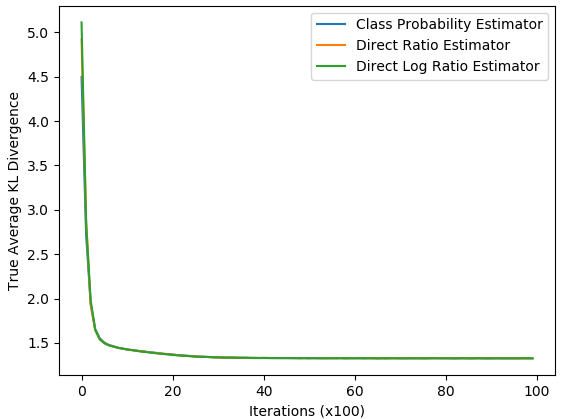
\includegraphics[width=\linewidth]{truklmins/PCADVvsPCADVexpvsPCADVgudlog.png}
\caption{GAN Divergence}
\end{subfigure}
\begin{subfigure}{0.49\textwidth}
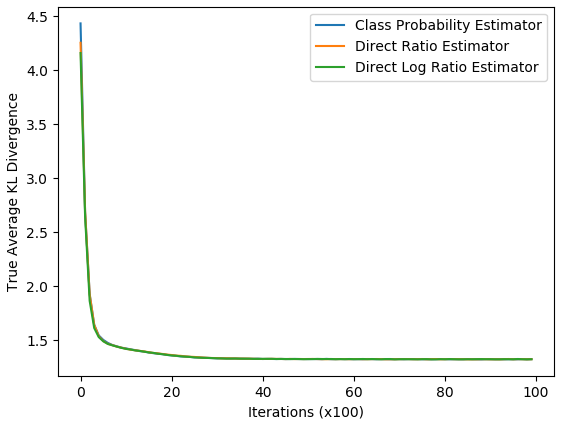
\includegraphics[width=\linewidth]{truklmins/PCKLDvsPCKLexpvsPCKLgudlog.png}
\caption{Reverse KL Divergence}
\end{subfigure}
\caption{Prior-Contrastive Average KL Divergence}
\end{figure}
\begin{figure}
\begin{subfigure}{0.49\textwidth}
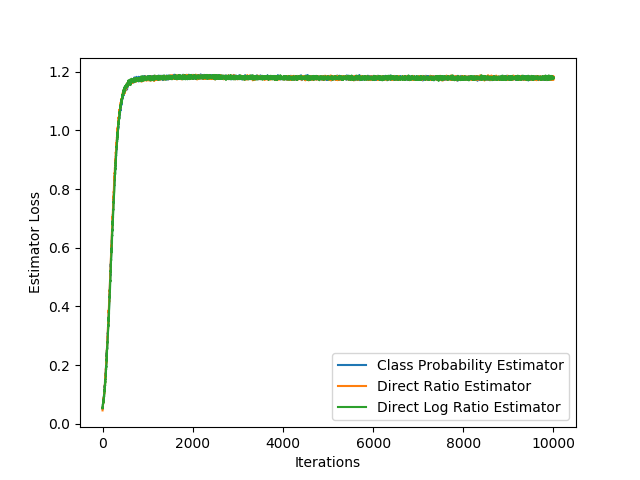
\includegraphics[width=\linewidth]{estimator_losses/PCADVvsPCADVexpvsPCADVgudlog.png}
\caption{GAN Divergence}
\end{subfigure}
\begin{subfigure}{0.49\textwidth}
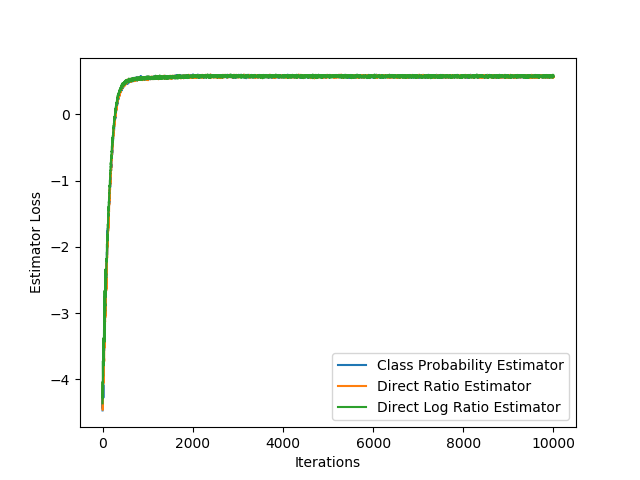
\includegraphics[width=\linewidth]{estimator_losses/PCKLDvsPCKLexpvsPCKLgudlog.png}
\caption{Reverse KL Divergence}
\end{subfigure}
\caption{Prior-Contrastive Estimator Loss}
\end{figure}
\begin{figure}
\begin{subfigure}{0.49\textwidth}
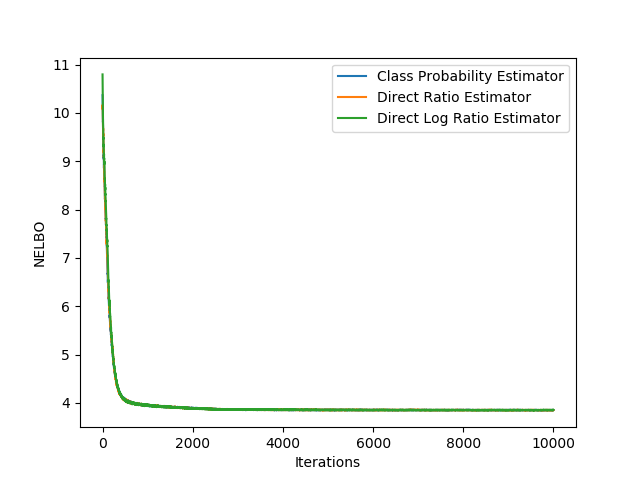
\includegraphics[width=\linewidth]{nelbos/PCADVvsPCADVexpvsPCADVgudlog.png}
\caption{GAN Divergence}
\end{subfigure}
\begin{subfigure}{0.49\textwidth}
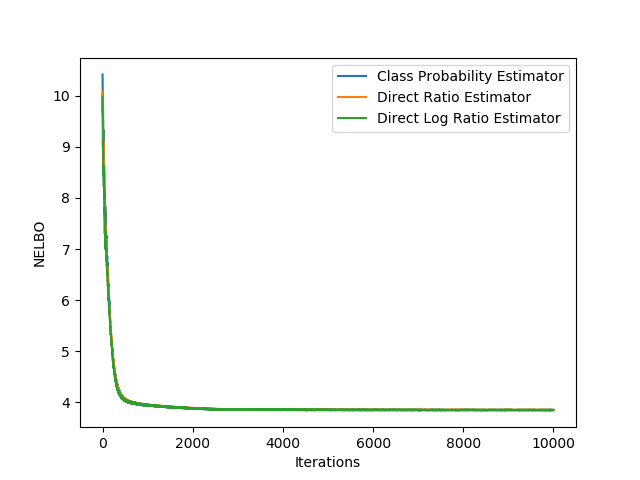
\includegraphics[width=\linewidth]{nelbos/PCKLDvsPCKLexpvsPCKLgudlog.png}
\caption{Reverse KL Divergence}
\end{subfigure}
\caption{Prior-Contrastive NELBO}
\end{figure}
\begin{figure}
\begin{subfigure}{0.49\textwidth}
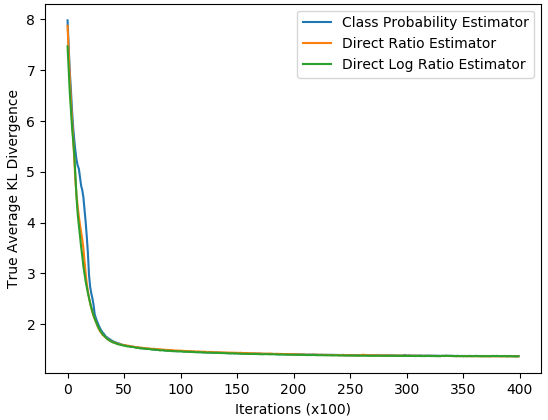
\includegraphics[width=\linewidth]{truklmins/JCADVvsJCADVexpvsJCADVgudlog.png}
\caption{GAN Divergence}
\end{subfigure}
\begin{subfigure}{0.49\textwidth}
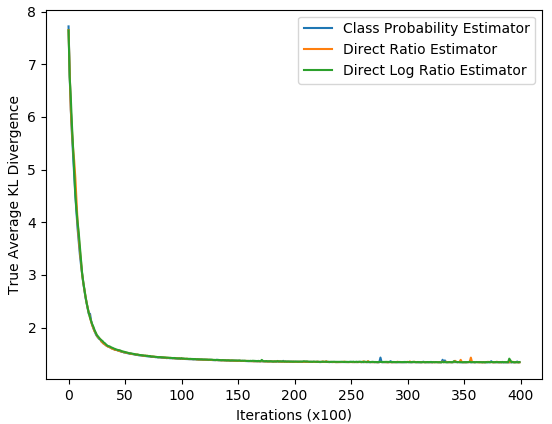
\includegraphics[width=\linewidth]{truklmins/JCKLDvsJCKLexpvsJCKLgudlog.png}
\caption{Reverse KL Divergence}
\end{subfigure}
\caption{Joint-Contrastive Average KL Divergence}
\end{figure}
\begin{figure}
\begin{subfigure}{0.49\textwidth}
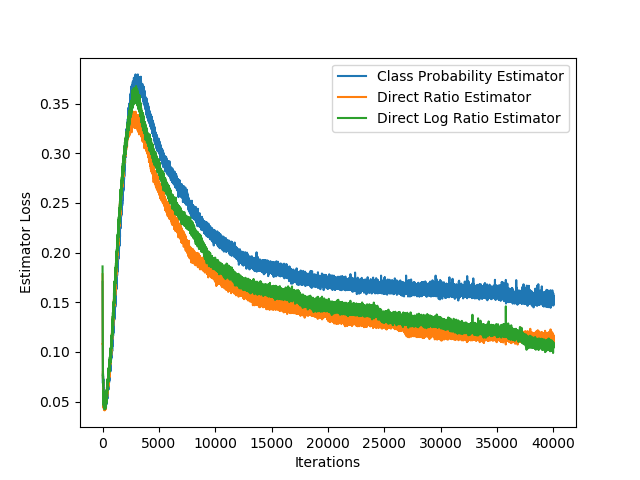
\includegraphics[width=\linewidth]{estimator_losses/JCADVvsJCADVexpvsJCADVgudlog.png}
\caption{GAN Divergence}
\end{subfigure}
\begin{subfigure}{0.49\textwidth}
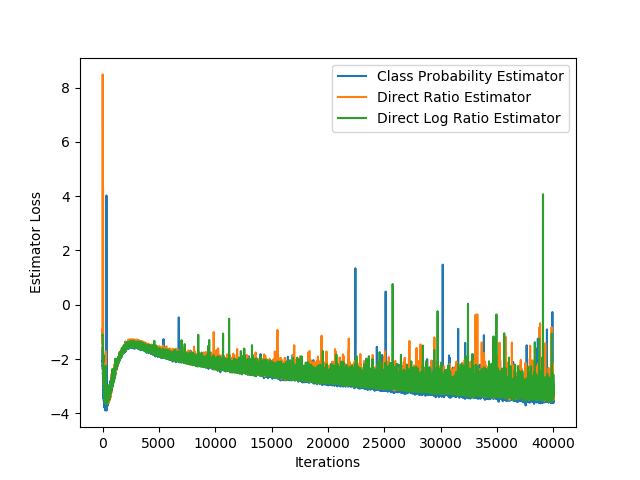
\includegraphics[width=\linewidth]{estimator_losses/JCKLDvsJCKLexpvsJCKLgudlog.png}
\caption{Reverse KL Divergence}
\end{subfigure}
\caption{Joint-Contrastive Estimator Loss}
\end{figure}

\begin{figure}
\begin{subfigure}{0.49\textwidth}
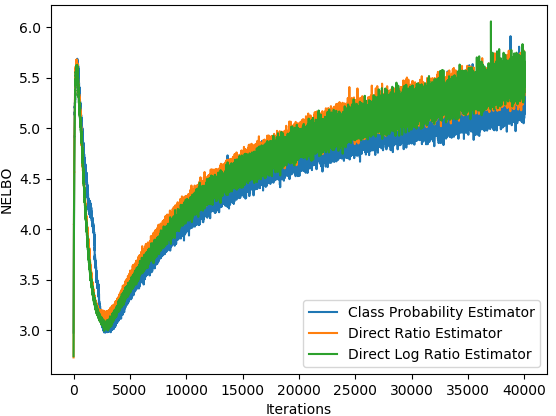
\includegraphics[width=\linewidth]{nelbos/JCADVvsJCADVexpvsJCADVgudlog.png}
\caption{GAN Divergence}
\end{subfigure}
\begin{subfigure}{0.49\textwidth}
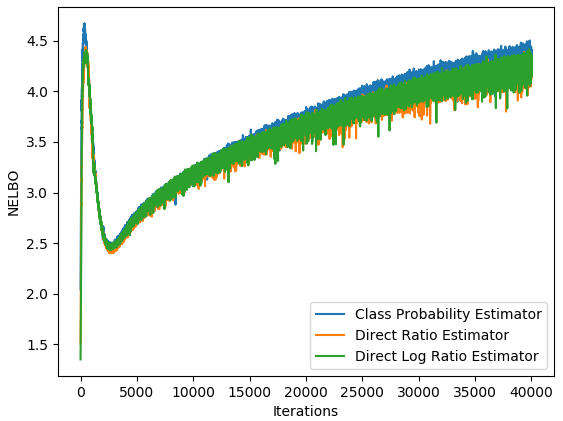
\includegraphics[width=\linewidth]{nelbos/JCKLDvsJCKLexpvsJCKLgudlog.png}
\caption{Reverse KL Divergence}
\end{subfigure}
\caption{Joint-Contrastive NELBO}
\end{figure}
\chapter{Comparing Undertrained Estimators}
Since all three estimator parametrisations have similar accuracies at optimality, it does not matter which one is chosen in that context. However, insufficient estimator training iterations can lead to an inaccurate estimation of the $NELBO$, reducing the speed at which the variational posterior converges. In this chapter, we first theoretically compare the rates of estimator convergence between the three parametrisations by analysing the bounds of the estimator outputs and the displacement in the optimal estimator output with each posterior optimisation step. We then perform an experiment in both prior-contrastive and joint-contrastive contexts comparing the performance of undertrained estimators with different parametrisations and f-divergence lower bounds.
\section{Theory}
\subsection{Estimator Bounds}
Consider the bounds on the estimator outputs. The class probability estimator $D_\alpha(u)\simeq \frac{q(u)}{q(u)+p(u)}$ is bound in $(0,1)$, so from any arbitrary starting point in the same space, very few optimization steps are required to reach the global minimum. On the other hand, the direct ratio estimator $r_\alpha(u)\simeq \frac{q(u)}{p(u)}$ is bound in $\R^+ \backslash \{0\}$, and the direct log ratio estimator $T_\alpha(u) \simeq \log \frac{q(u)}{p(u)}$ can take any value in $\R$, so optimization can take many iterations if the difference between the estimator's initial and optimal values is too large. This can be problematic if there are insufficient iterations of optimizing the estimator, particularly in the initialization stage: the estimator may not properly converge and the posterior will be trained with an inaccurate density ratio estimation. Essentially, the gradient descent convergence can be improved by using an appropriate transformation \citep{lecun}.

By converting the loss functions to integral form, we are able to visualise the bounds on the loss function output by fixing $q(u)$ and $p(u)$ as arbitrary values in $(0,1)$, and plotting the functional inside the integral. Figure 9.1 on page 75 depicts plots of estimator outputs against the loss functional where $q(u)=p(u)=0.5$.
\begin{example}
In this example we formulate the loss functional plotted in Figure 9.1 (a): the class probability estimator $D_\alpha(u)$ derived from the GAN divergence. The relevant estimator loss function is:
\begin{align*}
-\E_{q(u)}[\log D_\alpha(u)]-\E_{p(u)}[\log (1-D_\alpha(u))]&=\int_\R -q(u)\log D_\alpha(u)\\
&\quad \quad -p(u)\log(1-D_\alpha(u)) du\\
&=\int_\R -\frac{\log D_\alpha(u)+\log(1-D_\alpha(u))}{2}du.
\end{align*}
In the derivation above we have set $q(u)=p(u)=0.5$. Note we plot the functional inside the integral:
\[-\frac{\log D_\alpha(u)+\log(1-D_\alpha(u))}{2}.\]
\end{example}
\begin{figure}[h!]
\begin{subfigure}{0.49\textwidth}
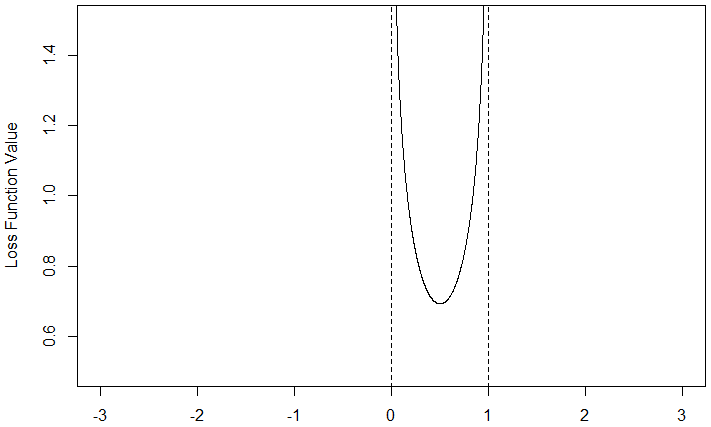
\includegraphics[width=\linewidth]{ADVD.png}
\caption{GAN Divergence - $D_\alpha(u)$}
\end{subfigure}
\begin{subfigure}{0.49\textwidth}
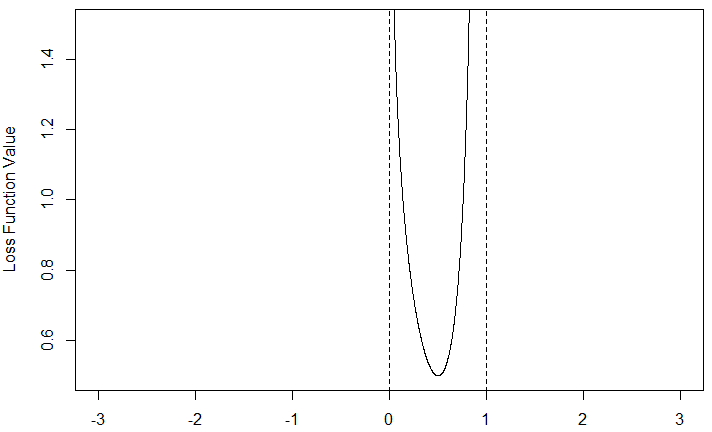
\includegraphics[width=\linewidth]{KLD.png}
\caption{Reverse KL Divergence - $D_\alpha(u)$}
\end{subfigure}
\begin{subfigure}{0.49\textwidth}
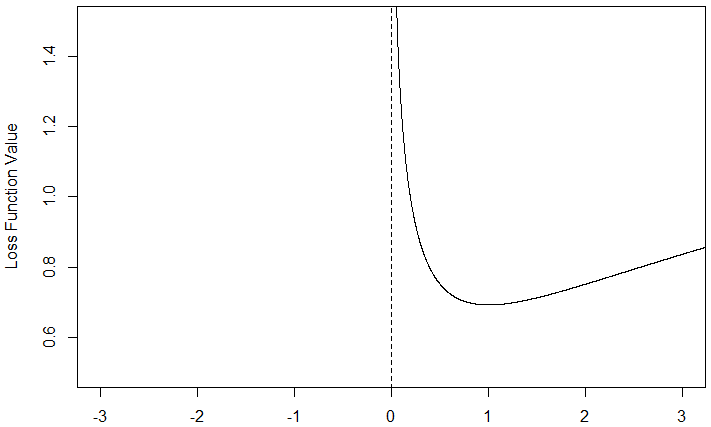
\includegraphics[width=\linewidth]{ADVR.png}
\caption{GAN Divergence - $r_\alpha(u)$}
\end{subfigure}
\begin{subfigure}{0.49\textwidth}
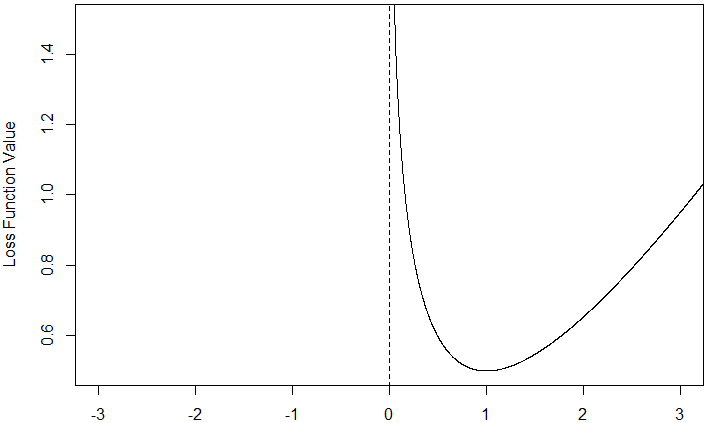
\includegraphics[width=\linewidth]{KLR.png}
\caption{Reverse KL Divergence - $r_\alpha(u)$}
\end{subfigure}
\begin{subfigure}{0.49\textwidth}
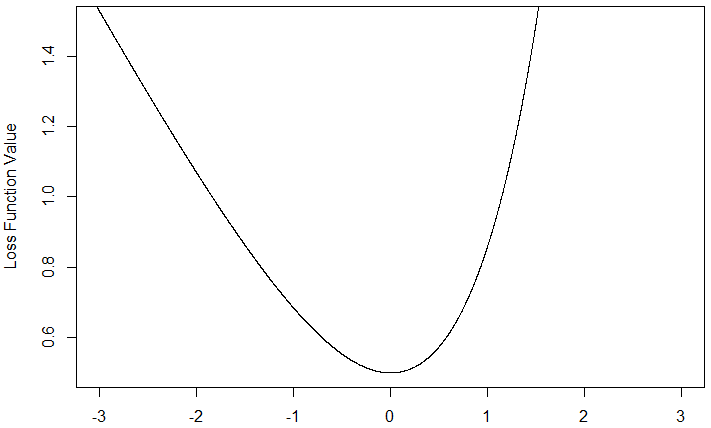
\includegraphics[width=\linewidth]{ADVT.png}
\caption{GAN Divergence - $T_\alpha(u)$}
\end{subfigure}
\begin{subfigure}{0.49\textwidth}
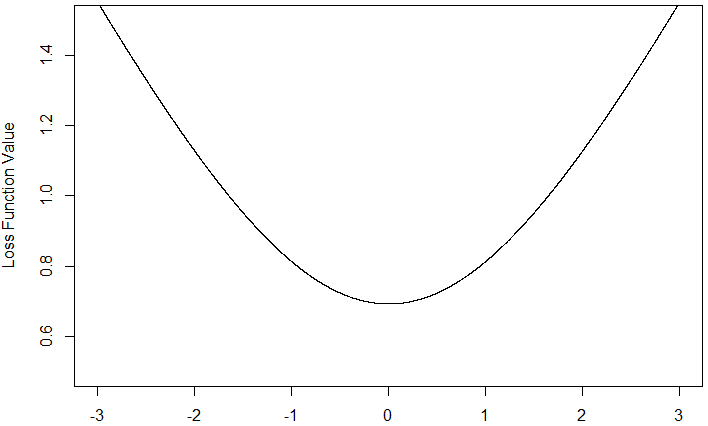
\includegraphics[width=\linewidth]{KLT.png}
\caption{Reverse KL Divergence - $T_\alpha(u)$}
\end{subfigure}
\caption{\small Above we have plotted the estimator output against its loss functional. The same x and y-axis scales are used for all plots. Due to the bounds, it is evident that the loss functionals using the class probability estimator $D_\alpha(u)$ are associated with the highest gradient values and therefore the fastest convergence. It is difficult to compare the direct ratio estimator $r_\alpha(u)$ and the direct log ratio estimator $T_\alpha(u)$, as the former estimator appears to have higher gradients when $q(u)<p(u)$, but slower convergence when $q(u)>p(u)$. Since the relative gradients of the graph can vary with the choice of $p(u)$ and $q(u)$, we cannot compare the f-divergences.}
\end{figure}
\subsection{First and Second Derivatives of Estimator Loss Functions}
To evaluate the effectiveness of gradient descent optimization in these algorithms, we formulate the first and second functional derivatives of the estimator loss functions.\\
\textbf{Reverse KL Divergence Upper Bound:}\\
Class Probability Estimator:
\begin{align*}
f_{KL}(u)&=-\E_{q(u)}\left(\log \frac{D(u)}{1-D(u)}\right)+\E_{p(u)}\left(\frac{D(u)}{1-D(u)}\right)\\
&=-\int_u q(u)\left(\log \frac{D(u)}{1-D(u)}\right)du+\int_u p(u)\left(\frac{D(u)}{1-D(u)}\right)du\\
\frac{df}{dD(u)}&=-\frac{q(u)}{D(u)}-\frac{q(u)}{1-D(u)}+\frac{p(u)}{1-D(u)}+\frac{p(u)D(u)}{(1-D(u))^2}\\
&=-\frac{q(u)}{D(u)}-\frac{q(u)}{1-D(u)}+\frac{p(u)}{(1-D(u))^2}\\
\frac{d^2f}{dD^2(u)}&=\frac{q(u)}{D^2(u)}-\frac{q(u)}{(1-D(u))^2}+\frac{2p(u)}{(1-D(u))^3}.
\end{align*}
\newpage
Direct Ratio Estimator:
\begin{align*}
f_{KL}(u)&=-\E_{q(u)}(\log r(u))+\E_{p(u)}r\\
&=-\int_u q(u)\log r(u) du+\int_u p(u)r(u)du\\
\frac{df}{dr(u)}&=-\frac{q(u)}{r(u)}+p(u)\\
\frac{d^2f}{dr^2(u)}&=\frac{q(u)}{r^2(u)}.
\end{align*}
Direct Log Ratio Estimator:
\begin{align*}
f_{KL}(u)&=-\E_{q(u)}[T(u)]+\E_{p(u)}[e^{T(u)}]\\
&=-\int_u q(u)T(u)du+\int_u p(u)e^{T(u)}du\\
\frac{df}{dT(u)}&=-q(u)+p(u)e^{T(u)}\\
\frac{d^2f}{dT^2(u)}&=p(u)e^{T(u)}.
\end{align*}
\textbf{GAN Divergence Upper Bound:}\\
Class Probability Estimator:
\begin{align*}
f_{CPE}(u)&=-\E_{q(u)}[\log D(u)]-\E_{p(u)}[\log (1-D(u))]\\
&=-\int_u q(u)\log D(u) du -\int_u p(u)\log(1-D)du\\
\frac{df}{dD(u)}&=-\frac{q(u)}{D(u)}+\frac{p(u)}{1-D(u)}\\
\frac{d^2f}{dD^2(u)}&=\frac{q(u)}{D^2(u)}+\frac{p(u)}{(1-D(u))^2}.
\end{align*}
Direct Ratio Estimator:
\begin{align*}
f_{CPE}(u)&=-\E_{q(u)}\left[\log \frac{r(u)}{r(u)+1}\right]+\E_{p(u)}\left[\log(r(u)+1)\right]\\
&=-\int_u q(u)\left[\log \frac{r(u)}{r(u)+1}\right]du+\int_u p(u)\left[\log(r(u)+1)\right]du\\
\frac{df}{dr(u)}&=-\frac{q(u)}{r(u)}+\frac{q(u)}{r(u)+1}+\frac{p(u)}{r(u)+1}\\
\frac{d^2f}{dr^2(u)}&=\frac{q(u)}{r^2(u)}-\frac{q(u)}{(r(u)+1)^2}-\frac{p(u)}{(r(u)+1)^2}.
\end{align*}
Direct Log Ratio Estimator:
\begin{align*}
f_{CPE}(u)&=-\E_{q(u)}[T(u)-\log(e^{T(u)}+1)]+\E_{p(u)}[\log(e^{T(u)}+1)]\\
&=\int_u q(u)[\log(e^{T(u)}+1)-T(u)] du+\int_u p(u)[\log(e^{T(u)}+1)]du\\
\frac{df}{dT(u)}&=-q(u)+\frac{(q(u)+p(u))e^{T(u)}}{e^{T(u)}+1}\\
\frac{d^2f}{dT^2(u)}&=\frac{(q(u)+p(u))\exp(T(u))}{e^{T(u)}+1}-\frac{(q(u)+p(u))e^{2T(u)}}{(e^{T(u)}+1)^2}\\
&=\frac{(q(u)+p(u))(e^{2T(u)}+e^{T(u)})-(q(u)+p(u))e^{2T(u)}}{(e^{T(u)}+1)^2}\\
&=\frac{(q(u)+p(u))e^{T(u)}}{(e^{T(u)}+1)^2}.
\end{align*}
Recall that both divergences attain the same global minimum, which is a parametrization of the estimator, and that these estimators are optimized via stochastic gradient descent. Thus, for a fixed estimator parametrization, the divergences will have varying rates of convergence, which can be analyzed by observing the second derivative. The convergence rate of a gradient descent method is proportional to the size of its second derivative \citep{lecun}.

For most of the second derivatives, it is difficult to make a clear comparison, particularly with the direct log ratio estimator due to the exponential terms. However, it can be seen that within the GAN divergence, the second derivative of the class probability estimator is strictly superior to that of the direct ratio estimator. Also, the direct ratio estimator has a strictly greater second derivative when its loss function is bounded by the reverse KL divergence than with the GAN divergence.
As previously stated, the effectiveness of different f-divergence upper bounds has been tested in \citet{nowozin}. They found that the ideal f-divergence used for the estimator's loss function is the same f-divergence that is being minimized in the variational posterior training: in this case, it is the KL divergence. This provides support for our theory that the KL divergence is superior (at least in the direct ratio case).
\subsection{Displacement of Estimator Optimal Values}
Furthermore, we can also consider the effect of the posterior density displacement from each training step: every time $q_\phi(u)$ changes, the optimal value of the estimator also changes. Consequently, the estimator must take optimization steps to `catch up', but again, if the displacement is too significant, then the estimator may not converge in time.
\begin{lemma}
For a fixed displacement of the variational distribution $q(u)$, the class probability estimator's global minimum displaces less than the direct ratio estimator, that is, $|D^*_{n+1}-D^*_{n}|<|r^*_{n+1}-r^*_{n}|$:
\begin{proof}
Letting $\epsilon\neq0$ be the change in $q(u)$ with an optimization step, and noting that $|\epsilon|<q(u)$, we have
\begin{align*}
|D^*_{n+1}-D^*_{n}|&=\left|\frac{q(u)+\epsilon}{q(u)+\epsilon+p(u)}-\frac{q(u)}{q(u)+p(u)}\right|\\
&=\left|\frac{q^2(u)+q(u)p(u)+\epsilon q(u)+\epsilon p(u)}{(q(u)+\epsilon+p(u))(q(u)+p(u))}-\frac{q^2(u)+\epsilon q(u)+q(u)p(u)}{(q(u)+\epsilon+p(u))(q(u)+p(u))}\right|\\
&=\left|\frac{\epsilon p(u)}{(q(u)+\epsilon+p(u))(q(u)+p(u))}\right|\\
&=\left|\frac{\epsilon}{(q(u)+\epsilon+p(u))\left(\frac{q(u)}{p(u)}+1\right)}\right|\\
|r^*_{n+1}-r^*_{n}|&=\left|\frac{q(u)+\epsilon}{p(u)}-\frac{q(u)}{p(u)}\right|\\
&=\left|\frac{\epsilon}{p(u)}\right|.
\end{align*}
If $\epsilon>0$, then
\[|D^*_{n+1}-D^*_{n}|<|r^*_{n+1}-r^*_{n}|\text{ as }(q(u)+\epsilon+p(u))\left(\frac{q(u)}{p(u)}+1\right)>p(u).\]
If $\epsilon<0$, then recalling that $|\epsilon| < q(u) < q(u)+p(u)$,
\begin{align*}
(q(u)+\epsilon+p(u))(\frac{q(u)}{p(u)}+1)&=\frac{q^2(u)}{p(u)}+2q(u)+p(u)+\epsilon \left(\frac{q(u)}{p(u)}+1\right)\\
&=(q(u)+\epsilon)\left(\frac{q(u)}{p(u)}+1\right)+q(u)+p(u)\\
&>p(u)
\end{align*}
\end{proof}
\end{lemma}
\begin{remark}
The class probability estimator $D_\alpha(u)$ has more accurate density ratio estimation than the direct ratio estimator $r_\alpha(u)$ when the estimators are undertrained.
\end{remark}
For the direct log ratio estimator, we have
\begin{align*}
|T^*_{n+1}-T^*_{n}|&=\left|\log \frac{q(u)+\epsilon}{p(u)}-\log \frac{q(u)}{p(u)}\right|\\
&=\left|\log \frac{q(u)+\epsilon}{q(u)}\right|
\end{align*}
It is difficult to make a direct comparison with the other displacement expressions.

\section{Experiment Outline}
In this experiment, we aim to confirm our theory that the estimator parametrisations have differing density ratio estimation accuracies when improperly trained, also determining which undertrained estimator is the most accurate by observing the convergence of the variational posterior.

The same ``Continuous Sprinkler" experimental setup is used, but with several changes to the training parameters. We significantly reduce the amount of estimator training, lowering the estimator training rate to 0.00004 and the estimator steps before each posterior iteration to 11 for both contrastive settings. We also increase the posterior training rate to 0.0002 and to account for this change, the number of optimization steps of the variational distribution is reduced to 2000 for the prior-contrastive context and 4000 in the joint-contrastive algorithms. 
\section{Results}
From Table 9.1, it is immediately clear that using the reverse KL divergence to derive the lower bound for the estimator loss function leads to significantly higher posterior convergence, again supporting our experimental results in Chapter 8. For each fixed contrastive context and f-divergence lower bound, the class probability estimator $D_\alpha(z,x)$ consistently demonstrates the lowest mean KL divergence, followed by the direct ratio estimator $r_\alpha (z,x)$ and the direct log ratio estimator $T_\alpha(z,x)$. This is consistent with the theory we present in Section 9.1, but the significance of the results varies depending on the comparison made.

The differences between the prior-contrastive estimators are relatively insignificant, but this is likely because the variational posterior weights $\phi$ are optimised with respect to a likelihood term $-\E_{q^*(x)\pi(\epsilon)}[\log p(x|\mathcal{G}_\phi(\epsilon;x))]$ in addition to the density ratio $\E_{q^*(x)q_\phi(z|x)}\left[\log \frac{q_\phi(z|x)}{p(z)}\right]$, so convergence is less impacted by an inaccurate density ratio estimation. It should be noted that the standard deviation of the results is relatively high: this is partially due to the stochastic nature of the optimisation. Therefore we consider a difference of half a standard deviation between the mean KL divergences as significant. In the joint-contrastive setting, there is a significant difference between the three estimators when the reverse KL bound is used. However, when the GAN divergence is used to formulate the estimator loss function, only the direct log ratio estimator demonstrates significantly worse posterior convergence than the other two estimators.
\begin{table}[h]
\centering
\begin{tabular}{|c|c|c|}
\hline
Algorithm & Mean KL Divergence & Standard Deviation\\
\hline
PC Reverse KL - $D_\alpha(z,x)$ & 1.3572 & 0.0136\\
\hline
PC Reverse KL - $r_\alpha(z,x)$ & 1.3607 & 0.0199\\
\hline
PC Reverse KL - $T_\alpha(z,x)$ & 1.3641 & 0.0141\\
\hline
PC GAN - $D_\alpha(z,x)$ & 1.3788 & 0.0258\\
\hline
PC GAN - $r_\alpha(z,x)$ & 1.3811 & 0.0365\\
\hline
PC GAN - $T_\alpha(z,x)$ & 1.3849 & 0.0450\\
\hline
\end{tabular}
\caption{Prior-Contrastive Results}
\end{table}
\begin{table}[h]
\centering
\begin{tabular}{|c|c|c|}
\hline
Algorithm & Mean KL Divergence & Standard Deviation\\
\hline
JC Reverse KL - $D_\alpha(z,x)$ & 1.3786 & 0.0286\\
\hline
JC Reverse KL - $r_\alpha(z,x)$ & 1.3934 & 0.0410\\
\hline
JC Reverse KL - $T_\alpha(z,x)$ & 1.4133 & 0.0597\\
\hline
JC GAN - $D_\alpha(z,x)$ & 1.4017 & 0.0286\\
\hline
JC GAN - $r_\alpha(z,x)$ & 1.4086 & 0.0555\\
\hline
JC GAN - $T_\alpha(z,x)$ & 1.4214 & 0.0518\\
\hline
\end{tabular}
\caption{Joint-Contrastive Results}
\end{table}

Due to the relatively large initial drop in average KL divergence, it is difficult to find any trends between the estimators from the corresponding graphs. It can however be seen that there is a faster initial drop in the `true' KL divergence when the GAN divergence is used for the estimator loss function. This is consistent with the estimator loss and NELBO plots: the reverse KL divergence bound experiences initial fluctuations and stabilises after 500 iterations, whilst the GAN divergence bound is relatively stable throughout the entire runtime. Despite this, the reverse KL divergence bound demonstrates superior overall convergence, reinforcing the results in Chapter 7, which suggest that estimators trained by it are more accurate density ratio estimators. However, these results imply that this is only the case when the estimator reaches stability.

In Figures 9.8 (a) and 9.9 (a), we notice that the direct ratio estimator plots significantly vary from the other two estimators, and that they are much more unstable. This does not appear to impact the posterior convergence, as it has a similar mean KL divergence with the class probability estimator. Again, it is unclear why the NELBO plot increases over the majority of the iterations in the joint-contrastive setting.
\newpage
\begin{figure}
\begin{subfigure}{0.49\textwidth}
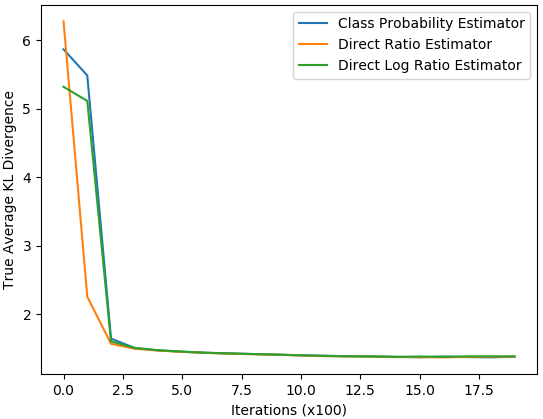
\includegraphics[width=\linewidth]{part2truklmins/PCADVvsPCADVexpvsPCADVgudlog.png}
\caption{GAN Divergence}
\end{subfigure}
\begin{subfigure}{0.49\textwidth}
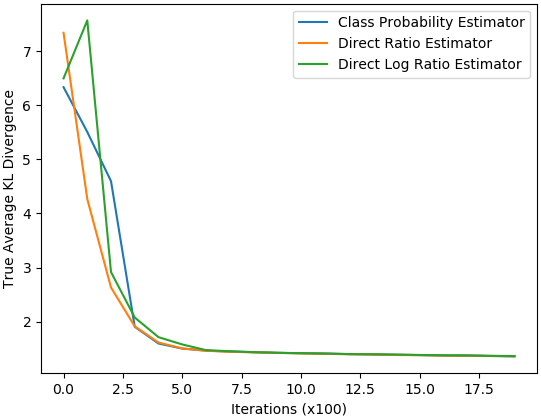
\includegraphics[width=\linewidth]{part2truklmins/PCKLDvsPCKLexpvsPCKLgudlog.png}
\caption{Reverse KL Divergence}
\end{subfigure}
\caption{Prior-Contrastive Average KL Divergence}
\end{figure}

\begin{figure}
\begin{subfigure}{0.49\textwidth}
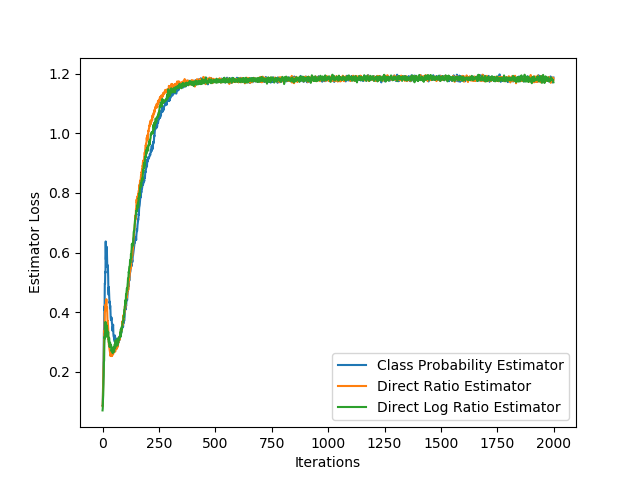
\includegraphics[width=\linewidth]{part2estimatorlosses/PCADVvsPCADVexpvsPCADVgudlog.png}
\caption{GAN Divergence}
\end{subfigure}
\begin{subfigure}{0.49\textwidth}
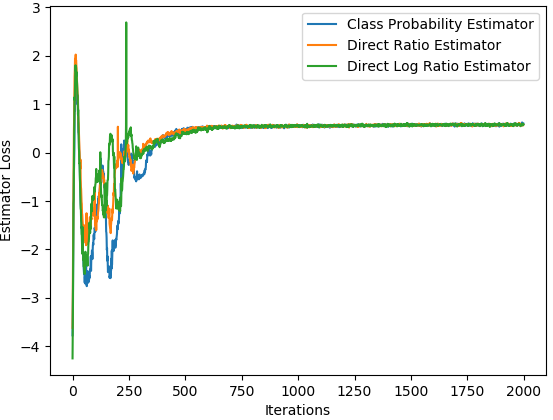
\includegraphics[width=\linewidth]{part2estimatorlosses/PCKLDvsPCKLexpvsPCKLgudlog.png}
\caption{Reverse KL Divergence}
\end{subfigure}
\caption{Prior-Contrastive Estimator Loss}
\end{figure}
\begin{figure}
\begin{subfigure}{0.49\textwidth}
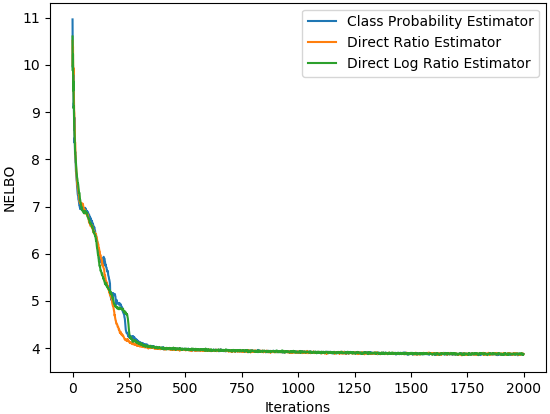
\includegraphics[width=\linewidth]{part2nelbos/PCADVvsPCADVexpvsPCADVgudlog.png}
\caption{GAN Divergence}
\end{subfigure}
\begin{subfigure}{0.49\textwidth}
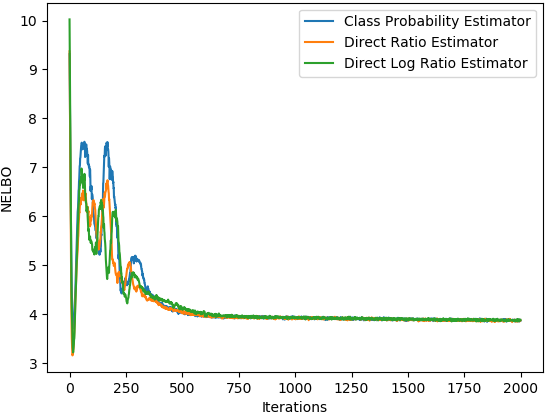
\includegraphics[width=\linewidth]{part2nelbos/PCKLDvsPCKLexpvsPCKLgudlog.png}
\caption{Reverse KL Divergence}
\end{subfigure}
\caption{Prior-Contrastive NELBO}
\end{figure}
\begin{figure}
\begin{subfigure}{0.49\textwidth}
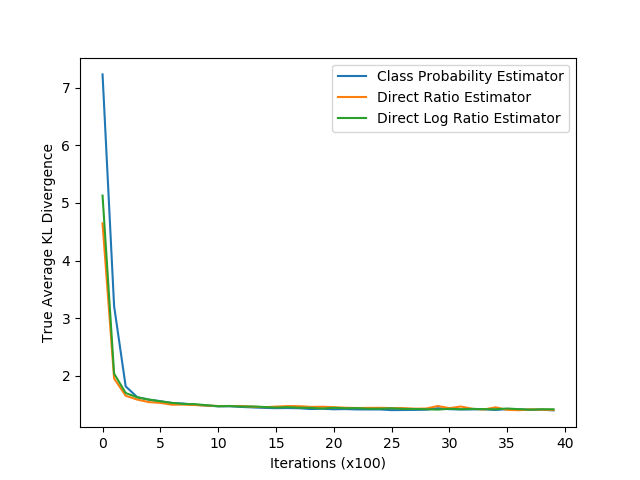
\includegraphics[width=\linewidth]{part2truklmins/JCADVvsJCADVexpvsJCADVgudlog.png}
\caption{GAN Divergence}
\end{subfigure}
\begin{subfigure}{0.49\textwidth}
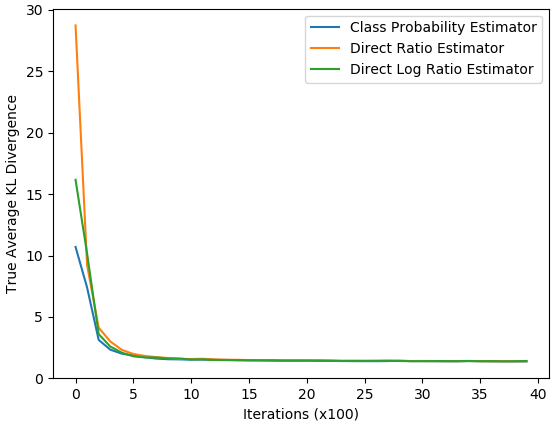
\includegraphics[width=\linewidth]{part2truklmins/JCKLDvsJCKLexpvsJCKLgudlog.png}
\caption{Reverse KL Divergence}
\end{subfigure}
\caption{Joint-Contrastive Average KL Divergence}
\end{figure}
\begin{figure}
\begin{subfigure}{0.49\textwidth}
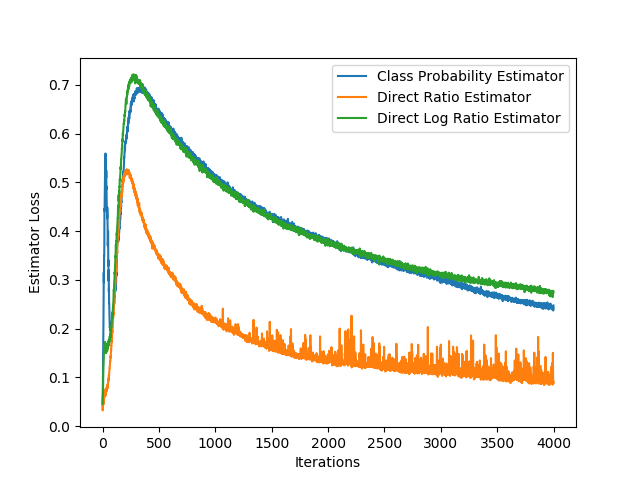
\includegraphics[width=\linewidth]{part2estimatorlosses/JCADVvsJCADVexpvsJCADVgudlog.png}
\caption{GAN Divergence}
\end{subfigure}
\begin{subfigure}{0.49\textwidth}
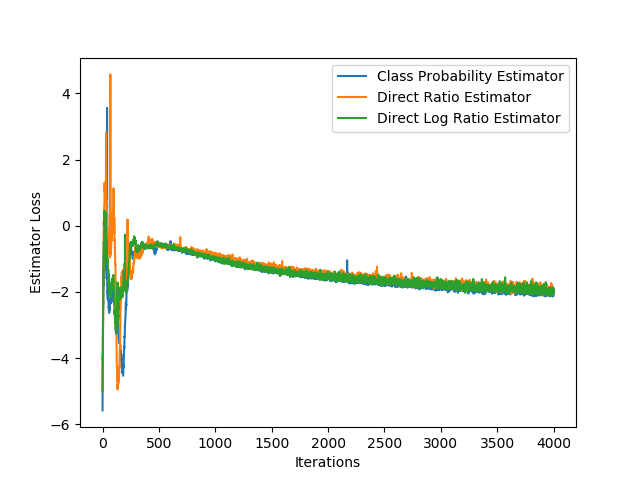
\includegraphics[width=\linewidth]{part2estimatorlosses/JCKLDvsJCKLexpvsJCKLgudlog.png}
\caption{Reverse KL Divergence}
\end{subfigure}
\caption{Joint-Contrastive Estimator Loss}
\end{figure}
\begin{figure}
\begin{subfigure}{0.49\textwidth}
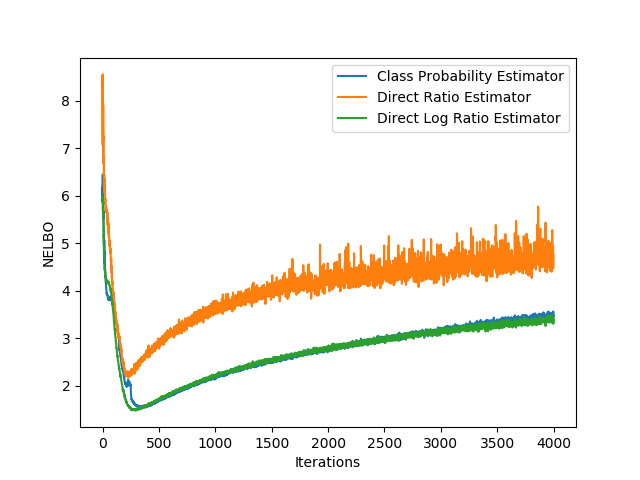
\includegraphics[width=\linewidth]{part2nelbos/JCADVvsJCADVexpvsJCADVgudlog.png}
\caption{GAN Divergence}
\end{subfigure}
\begin{subfigure}{0.49\textwidth}
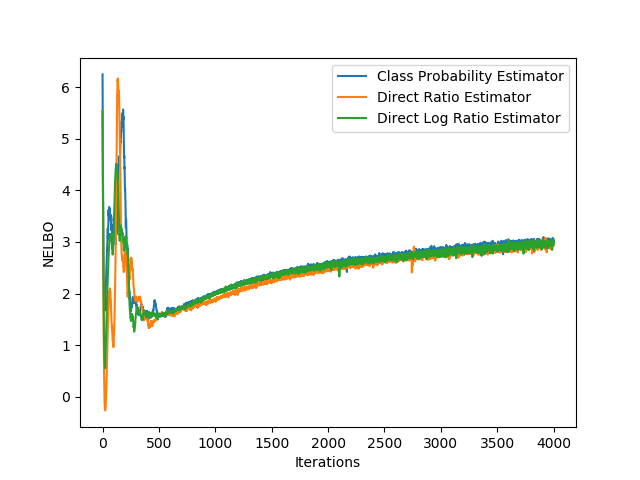
\includegraphics[width=\linewidth]{part2nelbos/JCKLDvsJCKLexpvsJCKLgudlog.png}
\caption{Reverse KL Divergence}
\end{subfigure}
\caption{Joint-Contrastive NELBO}
\end{figure}
\newpage
\chapter{Data Generation - (MNIST image generation)}
In this chapter we compare the different f-divergence bounds and estimator parametrisations in the density ratio estimation involved with data generation. Specifically, we use the MNIST dataset: a popular dataset used in machine learning algorithms. Again, we undertrain the estimators to determine which parametrisation performs the best. The primary goals of this experiment are to confirm the conclusions presented in Chapter 9, and to possibly gain further insights by applying the algorithms to a different experimental setting. Due to limited experimental time, we only test the prior-contrastive algorithms. We repeat the experiment with two different latent spaces, one with 2 dimensions and one with 10 dimensions, to determine if the dimensionality of the densities in the density ratio $\frac{q_\phi(z|x)}{p(z)}$ has any effect on the results.
\section{Experiment Outline}
The MNIST (Modified National Institute of Standards and Technology) dataset is widely used for testing machine learning algorithms related to image analysis. It contains 60,000 labelled training images and 10,000 testing images of handwritten digits, each greyscale and of 28x28 pixel size. A sample of the images can be seen in Figure 10.1. Our algorithms do not require the images to be labelled so we combine the two image sets and ignore the labelling.
\begin{figure}[b]
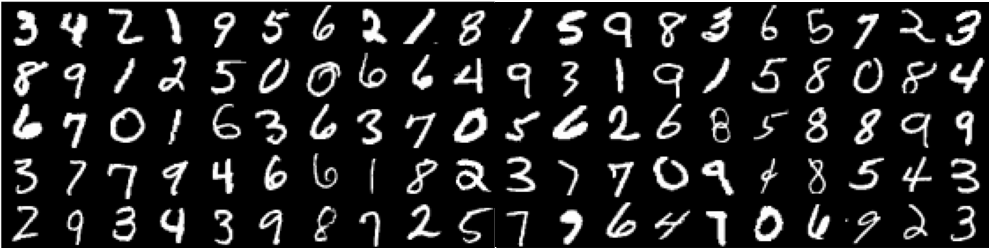
\includegraphics[width=\linewidth]{mnist-digits-small.png}
\caption{Samples from the MNIST Dataset}
\end{figure}
In this problem, we aim to generate new MNIST images indistinguishable from those in the original dataset. To do so, we use the ``Adversarial Variational Bayes" variation of the autoencoder as described in Section 3.9.1. Recall that the associated optimisation problem is:
\[\min_{\phi,\theta}\E_{q^*(x)}\left[-\E_{q_\phi(z|x)}[\log p_\theta(x|z)]+KL(q_\phi(z|x)\|p(z))\right].\]
We therefore have three neural networks:
\begin{itemize}
\item An encoder network $\mathcal{G}_\phi(\epsilon;x)$ that outputs samples from the variational posterior $q_\phi(z|x)$, effectively creating a latent representation of a data sample $x$.
\begin{figure}[h!]
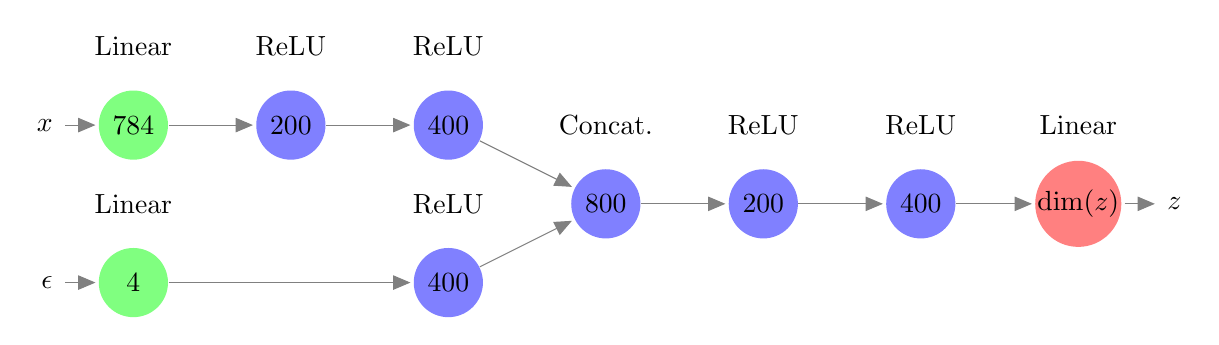
\begin{tikzpicture}[shorten >=1pt,->,draw=black!50, node distance=2.5cm]
    \tikzstyle{every pin edge}=[<-,shorten <=1pt]
    \tikzstyle{neuron}=[circle,fill=black!25,minimum size=25pt,inner sep=0pt]
    \tikzstyle{input neuron}=[neuron, fill=green!50];
    \tikzstyle{output neuron}=[neuron, fill=red!50];
    \tikzstyle{hidden neuron}=[neuron, fill=blue!50];
    \tikzstyle{annot} = [text width=4em, text centered]
    
	%\node[input neuron, pin=left:Bias] (I-0) at (0,0) {$x_0$};
    % Draw the input layer nodes
    %\foreach \name / \y in {1,...,3}
    % This is the same as writing \foreach \name / \y in {1/1,2/2,3/3,4/4}
    \node[input neuron, pin=left:$x$] (I-1) at (0,-1) {$784$};
	\node[input neuron, pin=left:$\epsilon$] (I-2) at (0,-3) {$4$};

    \path[yshift=0cm] node[hidden neuron] (H-11) at (2.0cm,-1) {$200$};
	\path[yshift=0cm] node[hidden neuron] (H-12) at (4.0cm,-1) {$400$};
    \path[yshift=0cm] node[hidden neuron] (H-2) at (4.0cm,-3) {$400$};
    \path[yshift=0cm] node[hidden neuron] (H-3) at (6.0cm,-2) {$800$};
    \path[yshift=0cm] node[hidden neuron] (H-31) at (8.0cm,-2) {$200$};
    \path[yshift=0cm] node[hidden neuron] (H-32) at (10.0cm,-2) {$400$};
	\path[yshift=0cm] node[output neuron,pin={[pin edge={->}]right:$z$}] (O) at (12.0cm, -2) {dim$(z)$};
    \path (I-1) edge (H-11);
    \path (H-11) edge (H-12);
	\path (I-2) edge (H-2);
	\path (H-12) edge (H-3);
	\path (H-2) edge (H-3);
	\path (H-3) edge (H-31);
	\path (H-31) edge (H-32);
	\path (H-32) edge (O);
    % Annotate the layers
    \node[annot,above of=I-1, node distance=1cm] {Linear};
    \node[annot,above of=I-2, node distance=1cm] {Linear};
    \node[annot,above of=H-11, node distance=1cm] {ReLU};
    \node[annot,above of=H-12, node distance=1cm] {ReLU};
    \node[annot,above of=H-2, node distance=1cm] {ReLU};
    \node[annot,above of=H-3, node distance=1cm] {Concat.};
    \node[annot,above of=H-31, node distance=1cm] {ReLU};
    \node[annot,above of=H-32, node distance=1cm] {ReLU};
    \node[annot,above of=O, node distance=1cm] {Linear};
\end{tikzpicture}
\caption{\small This figure illustrates the structure of the generator network $\mathcal{G}(x,\bm{\epsilon})$ used in the MNIST data generation experiment. The notation used in the figure is the same as in Figures 5.2 and 5.3, and overall the network structure is very similar except significantly more nodes are used, suiting the higher dimensionality of the data. The dimensionality of latent variable $z$ is either 2 or 10 depending on the experimental setting. We have arbitrarily chosen the number of random noise inputs $\epsilon$ to be 4.}
\end{figure}
\item A decoder network representing the likelihood distribution $p_\theta(x|z)$ that reconstructs a data sample $x$ from a latent variable input $z$.
\begin{figure}[h!]
\centering
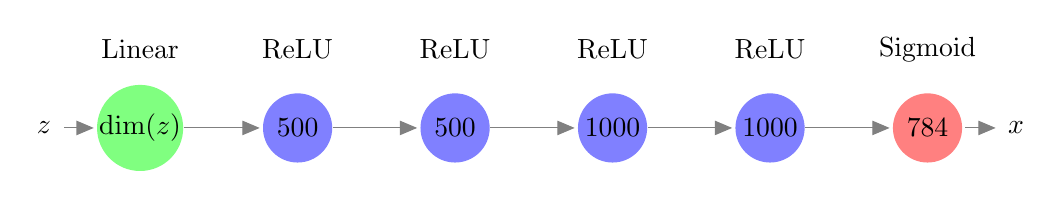
\begin{tikzpicture}[shorten >=1pt,->,draw=black!50, node distance=2.5cm]
    \tikzstyle{every pin edge}=[<-,shorten <=1pt]
    \tikzstyle{neuron}=[circle,fill=black!25,minimum size=25pt,inner sep=0pt]
    \tikzstyle{input neuron}=[neuron, fill=green!50];
    \tikzstyle{output neuron}=[neuron, fill=red!50];
    \tikzstyle{hidden neuron}=[neuron, fill=blue!50];
    \tikzstyle{annot} = [text width=4em, text centered]
    
	%\node[input neuron, pin=left:Bias] (I-0) at (0,0) {$x_0$};
    % Draw the input layer nodes
    %\foreach \name / \y in {1,...,3}
    % This is the same as writing \foreach \name / \y in {1/1,2/2,3/3,4/4}
    \node[input neuron, pin=left:$z$] (I-1) at (0,-1) {dim$(z)$};
    \path[yshift=0cm] node[hidden neuron] (H-1) at (2.0cm,-1) {$500$};
	\path[yshift=0cm] node[hidden neuron] (H-2) at (4.0cm,-1) {$500$};
	\path[yshift=0cm] node[hidden neuron] (H-3) at (6.0cm,-1) {$1000$};
	\path[yshift=0cm] node[hidden neuron] (H-4) at (8.0cm,-1) {$1000$};
	\path[yshift=0cm] node[output neuron,pin={[pin edge={->}]right:$x$}] (O) at (10.0cm, -1) {$784$};
    \path (I-1) edge (H-1);
    \path (H-1) edge (H-2);
	\path (H-2) edge (H-3);
	\path (H-3) edge (H-4);
	\path (H-4) edge (O);
    % Annotate the layers
    \node[annot,above of=I-1, node distance=1cm] {Linear};
    \node[annot,above of=H-1, node distance=1cm] {ReLU};
    \node[annot,above of=H-2, node distance=1cm] {ReLU};
    \node[annot,above of=H-3, node distance=1cm] {ReLU};
    \node[annot,above of=H-4, node distance=1cm] {ReLU};
    \node[annot,above of=O, node distance=1cm] {Sigmoid};
\end{tikzpicture}
\caption{\small This is a diagram of the decoder network used in the MNIST data generation experiment. A sigmoid output layer is used to map the network output to $(0,1)$, suiting the grayscale nature of the data. The amount of effective hidden layers is the same as in the encoder network, but there are significantly more nodes in each layer. This is because the objective of the program is to output relatively high dimensional image data. Although this problem involves image analysis, due to the relatively small image size we refrain from using convolutional layers. This is consistent with other similar MNIST experiments \citep{nowozin, bgan}.}
\end{figure}
\item A density ratio estimator network ($D_\alpha(z,x),r_\alpha(z,x)$ or $T_\alpha(z,x)$) used to evaluate the intractable $KL(q_\phi(z|x)\|p(z))$ term in the optimisation problem.
\begin{figure}[h!]

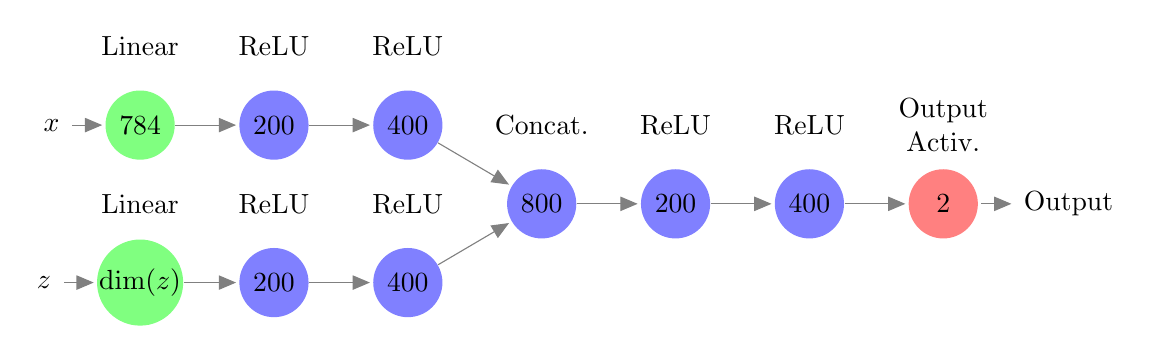
\begin{tikzpicture}[shorten >=1pt,->,draw=black!50, node distance=2.5cm]
    \tikzstyle{every pin edge}=[<-,shorten <=1pt]
    \tikzstyle{neuron}=[circle,fill=black!25,minimum size=25pt,inner sep=0pt]
    \tikzstyle{input neuron}=[neuron, fill=green!50];
    \tikzstyle{output neuron}=[neuron, fill=red!50];
    \tikzstyle{hidden neuron}=[neuron, fill=blue!50];
    \tikzstyle{annot} = [text width=4em, text centered]
    
	%\node[input neuron, pin=left:Bias] (I-0) at (0,0) {$x_0$};
    % Draw the input layer nodes
    %\foreach \name / \y in {1,...,3}
    % This is the same as writing \foreach \name / \y in {1/1,2/2,3/3,4/4}
    \node[input neuron, pin=left:$x$] (I-1) at (0,-1) {$784$};
	\node[input neuron, pin=left:$z$] (I-2) at (0,-3) {dim$(z)$};

    \path[yshift=0cm] node[hidden neuron] (H-11) at (1.7cm,-1) {$200$};
	\path[yshift=0cm] node[hidden neuron] (H-12) at (3.4cm,-1) {$400$};
	\path[yshift=0cm] node[hidden neuron] (H-21) at (1.7cm,-3) {$200$};
    \path[yshift=0cm] node[hidden neuron] (H-22) at (3.4cm,-3) {$400$};
    \path[yshift=0cm] node[hidden neuron] (H-3) at (5.1cm,-2) {$800$};
    \path[yshift=0cm] node[hidden neuron] (H-31) at (6.8cm,-2) {$200$};
    \path[yshift=0cm] node[hidden neuron] (H-32) at (8.5cm,-2) {$400$};
	\path[yshift=0cm] node[output neuron,pin={[pin edge={->}]right:Output}] (O) at (10.2cm, -2) {$2$};
    \path (I-1) edge (H-11);
    \path (H-11) edge (H-12);
	\path (I-2) edge (H-21);
	\path (H-21) edge (H-22);
	\path (H-12) edge (H-3);
	\path (H-22) edge (H-3);
	\path (H-3) edge (H-31);
	\path (H-31) edge (H-32);
	\path (H-32) edge (O);
    % Annotate the layers
    \node[annot,above of=I-1, node distance=1cm] {Linear};
    \node[annot,above of=I-2, node distance=1cm] {Linear};
    \node[annot,above of=H-11, node distance=1cm] {ReLU};
    \node[annot,above of=H-12, node distance=1cm] {ReLU};
    \node[annot,above of=H-21, node distance=1cm] {ReLU};
    \node[annot,above of=H-22, node distance=1cm] {ReLU};
    \node[annot,above of=H-3, node distance=1cm] {Concat.};
    \node[annot,above of=H-31, node distance=1cm] {ReLU};
    \node[annot,above of=H-32, node distance=1cm] {ReLU};
    \node[annot,above of=O, node distance=1cm] {Output Activ.};
\end{tikzpicture}
\caption{\small This figure depicts the estimator network for the MNIST data generation experiment. Depending on the estimator parametrisation, the output activation function is either sigmoid for the class probability estimator $D_\alpha(z,x)\simeq \frac{q_\phi(z|x)}{q_\phi(z|x)+p(z)}$, exponential for the direct ratio estimator $r_\alpha(z,x)\simeq \frac{q_\phi(z|x)}{p(z)}$ or linear for the direct log ratio estimator $T_\alpha(z,x)\simeq \log \frac{q_\phi(z|x)}{p(z)}$.}
\end{figure}
\end{itemize}
The program alternates between several iterations of estimator training and a simultaneous training step of the encoder and decoder weights.

Unlike the exact ``Adversarial Variational Bayes" specification in Section 3.9.1, we do not add random noise to the decoder, therefore resulting in a deterministic output. To express the likelihood term $\E_{q_\phi(z|x)}[\log p_\theta(x|z)]$ in the optimisation problem, we use the likelihood function of a Bernoulli distribution, with probability equal to the output of the decoder. This likelihood representation is common in literature, and is used for several reasons \citep{nowozin,bgan, tiao}:
\begin{itemize}
\item Image blurriness is reduced as there is no random noise in the pixel values.
\item We use the reconstruction error $\|x-\tilde{x}\|^2$ to evaluate convergence, so a noisy sample reconstruction can make it difficult to compare the algorithms.
\item In this experiment, we are primarily interested in the accuracy of the density ratio estimation between the variational posterior and the prior: this is independent of the decoder parametrisation.
\end{itemize}
\begin{figure}[h]
  \centering
  \tikz{ %
    \node[latent] (x) {$\bm{x}$} ; %
    \node[det, right=of x] (q) {$\mathcal{G}_\phi(\epsilon_1;\bm{x})$} ; %
    \node [latent, above=of q] (eps) {$\epsilon_1$} ;
    \node [latent, right=of q] (z) {$\bm{z}$} ;
    \node [det, right=of z] (p) {$p_\theta(\bm{x}|\bm{z})$} ;
    \node [latent, right=of p] (pout) {$\tilde{\bm{x}}$} ;
    \edge {x} {q} ; %
    \edge {q} {z}
    \edge {eps} {q} ;
    \edge {z} {p} ;
    \edge {p} {pout} ;
  }
   \caption{\small This diagram depicts the ``Adversarial Variational Bayes" formulation of the variational autoencoder used in the MNIST data generation experiment. Note that there is no random noise added to the decoder.}
\end{figure}

The network structure and parameters have been configured to be similar to the MNIST experiment performed in ``f-GAN: Training Generative Neural Samplers using Variational Divergence Minimization" by \citet{nowozin}: a large batch size of 2048 is used and for each network, a training rate of 0.0004 is used in the low dimensional configuration, whilst the high dimensional setting uses a training rate of 0.0001. Again, the estimator is pre-trained for 5000 iterations, afterwards the program alternates between 20 iterations of estimator optimizaton and 1 iteration of posterior training, for 4000 total posterior iterations. Like in the ``Sprinkler" experiments, the estimator loss and estimated NELBO at each posterior iteration was saved, and every 10 posterior iterations, 500 MNIST samples were passed through the autoencoder and the average reconstruction error $\|x-\tilde{x}\|^2$ was saved.
\section{Low Dimensional Experiment Results}
Table 10.1 below tabulates the mean and standard deviation of the autoencoder's final reconstruction error between the 30 experiment repetitions. The only notable observation is that the direct log ratio estimator trained with a GAN divergence leads to significantly higher reconstruction error. This is consistent throughout the 30 repetitions and is not due to any outlier instances, reinforcing the theory and conclusions in Chapter 9. We also note that the estimators trained with the reverse KL divergence have consistently lower reconstruction errors, and that the class probability estimator appears to give the most accurate density ratio estimation, followed by the direct ratio estimator and the direct log ratio estimator. However, the differences are insignificant, likely because the estimators experience a relatively higher level of training in comparison to the experiment in Chapter 9. Additionally, the presence of the likelihood term in the $NELBO$ loss function reduces the importance of correct density ratio estimation.
\begin{table}[h]
\centering
\begin{tabular}{|c|c|c|}
\hline
Algorithm & Mean Reconstruction Error & Standard Deviation\\
\hline
PC Reverse KL - $D_\alpha(z,x)$ & 0.08662 & 0.00154\\
\hline
PC Reverse KL - $r_\alpha(z,x)$ & 0.08710 & 0.00214\\
\hline
PC Reverse KL - $T_\alpha(z,x)$ & 0.08730 & 0.00157\\
\hline
PC GAN - $D_\alpha(z,x)$ & 0.08673 & 0.00129\\
\hline
PC GAN - $r_\alpha(z,x)$ & 0.08716 & 0.00151\\
\hline
PC GAN - $T_\alpha(z,x)$ & 0.10683 & 0.00199\\
\hline
\end{tabular}
\caption{Reconstruction Errors for the Low Dimensional MNIST Generation Experiment}
\end{table}
\newpage
\begin{figure}[t!]
\centering
\begin{subfigure}{0.49\textwidth}
\includegraphics[width=\linewidth]{part3reconerrors/PCADVvsPCADVexpvsPCADVgudlog.png}
\caption{GAN Divergence}
\end{subfigure}
\begin{subfigure}{0.49\textwidth}
\includegraphics[width=\linewidth]{part3reconerrors/PCKLDvsPCKLexpvsPCKLgudlog.png}
\caption{Reverse KL Divergence}
\end{subfigure}
\caption{\small In the above average KL divergence plots, the only noticeable feature is that the direct log ratio estimator in sub-figure (a) consistently has a higher reconstruction error for most of the iterations.}
\end{figure}

\begin{figure}[h!]
\centering
\begin{subfigure}{0.49\textwidth}
\includegraphics[width=\linewidth]{part3estimatorlosses/PCADVvsPCADVexpvsPCADVgudlog.png}
\caption{GAN Divergence}
\end{subfigure}
\begin{subfigure}{0.49\textwidth}
\includegraphics[width=\linewidth]{part3estimatorlosses/PCKLDvsPCKLexpvsPCKLgudlog.png}
\caption{Reverse KL Divergence}
\end{subfigure}
\caption{\small Noting the scale of the estimator loss plot in sub-figure (b), it is evident that the reverse KL divergence leads to unstable estimator training. Unlike the estimators plotted in Figure 9.3 (b), these estimators don't appear to stabilise after a certain period. Sub-figure (a) shows that the direct log ratio estimator loss is consistently higher than the other two estimators, correlating with its poorer reconstruction.}
\end{figure}
\begin{figure}[h!]
\centering
\begin{subfigure}{0.49\textwidth}
\includegraphics[width=\linewidth]{part3nelbos/PCADVvsPCADVexpvsPCADVgudlog.png}
\caption{GAN Divergence}
\end{subfigure}
\begin{subfigure}{0.49\textwidth}
\includegraphics[width=\linewidth]{part3nelbos/PCKLDvsPCKLexpvsPCKLgudlog.png}
\caption{Reverse KL Divergence}
\end{subfigure}
\caption{\small Despite the apparent instability of the estimators trained with the reverse KL divergence, the NELBO plot in sub-figure (b) is relatively consistent, leading to a smooth convergence as plotted in Figure 10.6 (b). The high estimator losses shown in Figure 10.7 (a) correspond to an overestimated NELBO as depicted in sub-figure (a).}
\end{figure}
\section{High Dimensional Experiment Results}
When the dimensionality of the latent space was increased to 10, the direct ratio and direct log ratio estimator loss functions involved quantities greater than the largest representable 64-bit floating point number, overflowing to \verb+Inf+ and outputting \verb+NaN+ for the remainder of the program runtime. This is because the density ratio $\frac{q_\phi(z|x)}{p(z)}$ increases with the dimensionality of the latent space, eventually reaching a value that is too large to be represented by a 64-bit float. The direct ratio estimator $r_\alpha(z,x)\simeq \frac{q_\phi(z|x)}{p(z)}$ therefore fails in this scenario. Now recall that the direct log ratio estimator loss function involves taking the exponential of the estimator output. For example, the loss function formulated by the reverse KL divergence is
\[-\E_{q^*(x)\pi(\epsilon)}[T_\alpha(\mathcal{G}(\epsilon;x),x)]+\E_{p(z)q^*(x)}[\exp(T_\alpha(z,x))].\]
So despite $T_\alpha(z,x)$ outputting the log of the density ratio, the exact density ratio is expressed in the loss function when the exponential is taken, causing the program to fail. On the other hand, the class probability estimator does not experience this problem as its output is bound in $(0,1)$.
\begin{lemma}
The class probability estimator network output before passing through the sigmoid activation function $g(x)=\frac{1}{1+e^{-x}}$ is the estimated log density ratio $\log \frac{q_\phi(z|x)}{p(z)}$.
\begin{proof}
Letting $x$ be the neural network output before being mapped to $(0,1)$, we have:
\begin{align*}
\frac{1}{1+e^{-x}}&\simeq\frac{q_\phi(z|x)}{p(z)+q_\phi(z|x)}\\
e^{-x}+1&\simeq\frac{p(z)+q_\phi(z|x)}{q_\phi(z|x)}\\
e^{-x}&\simeq\frac{p(z)}{q_\phi(z|x)}\\
x&\simeq\log \frac{q_\phi(z|x)}{p(z)}.
\end{align*}
\end{proof}
\end{lemma}
\begin{remark}
The calculations involved with the class probability estimator lie within the space of representable numbers by 64-bit, and even 32-bit floating point numbers.
\end{remark}
We can therefore conclude that the class probability estimator is superior in the sense that it is the only feasible parametrization. It remains to compare the f-divergence used to formulate the estimator loss function. The reconstruction errors are tabulated in Table 10.2 below.
\begin{table}[h]
\centering
\begin{tabular}{|c|c|c|}
\hline
Algorithm & Mean Reconstruction Error & Standard Deviation\\
\hline
PC Reverse KL - $D_\alpha(z,x)$ & 0.06470 & 0.01949\\
\hline
PC GAN - $D_\alpha(z,x)$ & 0.04440 & 0.00174\\
\hline
\end{tabular}
\caption{Reconstruction Errors for the High Dimensional MNIST Generation Experiment}
\end{table}\\
Here, the GAN divergence leads to significantly lower reconstruction error mean and standard deviation, contradicting the superiority of the reverse KL divergence shown in the previous experiments. An analysis of the plots in Figures 10.9-10.11 may explain this occurrence.
\begin{figure}[h]
\centering
\includegraphics[width=0.49\linewidth]{part4reconerrors/PCADVvsPCKLD.png}
\caption{\small This plot shows that the reconstruction error associated with the reverse KL divergence is consistently higher for the majority of the program runtime.}
\end{figure}
\begin{figure}[h]
\centering
\includegraphics[width=0.49\linewidth]{part4estimatorlosses/PCADVvsPCKLD.png}
\caption{\small The estimator loss corresponding to the reverse KL divergence appears to be extremely unstable for the entire program runtime, spiking to values exceeding $10^{14}$. On the other hand, the GAN divergence estimator loss appears to be relatively stable.}
\end{figure}
\begin{figure}[h]
\centering
\includegraphics[width=0.49\linewidth]{part4nelbos/PCADVvsPCKLD.png}
\caption{\small The instability of the reverse KL divergence estimator loss propagates to its NELBO estimation, which appears to fluctuate wildly in comparison to the GAN divergence's loss. This correlates to the superiority of the GAN divergence in this particular experiment. Again recalling Figures 9.3 and 9.6 (b), estimators formulated by the reverse KL divergence experience initial instability, but have more accurate density ratio estimation when stable. It is possible that the estimator in this experiment has not stabilised, leading to poorer network convergence. This may be due to the increased complexity of the distributions associated with the MNIST dataset, as opposed to the simplicity of the previous ``Sprinkler" problem.}
\end{figure}
\chapter{Discussion and Conclusion}
Leave this as a brainstorm list for now
\begin{itemize}
\item Of course many other problems and training parameters can be explored, variational inference and implicit models are used for more than inference and generation
\item More f-divergences can be explored (Nowozin, 2016)
\item Could test estimators for CycleGANs (joint-contrastive formulation for images) (Tiao, 2018)
\item Could take a step back from using neural networks to estimate the divergence, instead try divergence estimation via k-nearest-neighbour distances (Wang, 2009)
\item I don't know how denoisers work but they may be comparable to the methods discussed in this thesis (Huszar)
\item Hopefully in the future everyone will be using class probability estimators trained under the loss function formulated by the KL divergence :)
\end{itemize}


%%%%%%%%%%%%%%%%%%%%%%%%%%%%%%%%%%%%%%%%%%%%%%%%%%%%%%%%%%%%%%%%%%%%%%%%%%
\clearpage
\addcontentsline{toc}{chapter}{References}
\bibliographystyle{apalike}
\bibliography{bible}



\newpage
\appendix
\chapter{Kernel Density Estimation}
Kernel density estimation is a non-parametric method used to estimate the probability density function of a distribution, using only samples. It can therefore be used to estimate implicit distributions. For simplicity we only explain the univariate form of the kernel density estimator, though the multivariate form is used in this thesis.

Let $\{x^{(i)}\}^n_{i=1}$ be an independent and identically distributed sample from a distribution with unknown probability density function $f$. Its kernel density estimator is defined as
\[\hat{f}_h(x)=\frac{1}{nh}\sum^n_{i=1}K\left(\frac{x-x^{(i)}}{h}\right).\]
$K$ is the kernel, a symmetric non-negative weighting function that integrates to 1. Examples of kernel functions are:
\begin{itemize}
\item Epanechnikov: $K(u)=\frac{3}{4}(1-u^2), |u|\leq 1$
\item Uniform: $K(u)=\frac12, |u|\leq 1$
\item Gaussian: $K(u)=\frac{1}{\sqrt{2\pi}}\exp\left(-\frac{1}{2}u^2\right)$.
\end{itemize}
Typically, the Gaussian kernel is used due to its statistical properties, but the choice of kernel is not as important as the choice of $h$, the bandwidth.

The bandwidth $h>0$ acts as a smoothing parameter, determining the width of the kernel. If $h$ is too small, $\hat{f}$ will be 'undersmoothed' as too much weight is placed on the areas nearest the data-points, leading to a spiky estimate with high variance. On the other hand, if $h$ is too large, $\hat{f}$ will be 'oversmoothed' with too little weight on areas nearest to the data-points, resulting in a relatively flat estimate with high bias. It is therefore ideal to choose $h$ such that the mean integrated square error $MISE(h)=\E\left[\int(\hat{f}_h(x)-f(x))^2dx\right]$ is minimized. For a Gaussian kernel, this is approximately $h=1.06\hat{\sigma}n^{-1/5}$ where $\hat{\sigma}$ is the sample standard deviation. We omit the proof in this thesis.

The kernel density estimator works by placing a kernel on each data point and summing up the kernels to produce a smooth curve. Each point on the curve is essentially a weighted average of nearby data points. Regions of the curve with many data points will therefore have a high estimated probability density.
\end{document}





